\ProvidesFile{Communication.tex}[Межобъектное взаимодействие]


\section{Межобъектная коммуникация}
% TO DO

\subsection{Зачем?}
% TO DO

\paragraph{Стандартный код}

Давайте начнем с двух примеров того, как принято писать код
\begin{center}
\begin{tabular}{cc}
{
\begin{minipage}[\baselineskip]{8cm}
\begin{cppcode}[numbers = none]



int main() {
  Data1 input = read();
  Data2 result = apply_algorithm(input);
  print(result);
  return 0;
}
\end{cppcode}
\end{minipage}
}&{
\begin{minipage}[\baselineskip]{9cm}
\begin{cppcode}[numbers = none]
struct A {
  void process(const char* command) {
    parse(command); // set arg
    Data1 data = read(arg.file1);
    Data2 result = apply(data, arg.algorithm);
    write(result, arg.file2);
  }
  Command arg;
};
\end{cppcode}
\end{minipage}
}
\end{tabular}
\end{center}
Слева пример стандартного консольного приложения.
Оно состоит по сути из трех строчек
\begin{enumerate}
\item Считать данные и положить в \verb"input".

\item Применить к \verb"input" алгоритм и получить \verb"result".

\item Вывести \verb"result" на печать.
\end{enumerate}
Вся работа на каждом шаге делегируется трем различным функциям.
Я хочу обратить внимание на то, кто занимается передачей данных между тремя функциями.
За передачу данных и временные переменные отвечает сама функция \verb"main".
В примере справа происходит более или менее то же самое.
У класса \verb"A" есть метод \verb"process", который вызывает такие же три стадии:
\begin{enumerate}
\item Считать данные и положить в \verb"data".

\item Применить к \verb"data" алгоритм и получить \verb"result".

\item Вывести \verb"result" на печать.
\end{enumerate}
Отличие лишь в том, что теперь у нас есть состояние, хранящееся внутри класса \verb"A", которое может на что-то неявно повлиять.
И в этом случае за передачу данных между методами отвечает по сути класс \verb"A".
Если быть точнее, то надо сказать метод \verb"process".

Давайте отметим, что это стандартный способ писать код.
Мы так привыкли писать функции и классы.
Функции внутри себя передают данные между отдельными функциями.
Классы сами передают свои внутренние данные между разными методами.
В этом случае передача данных осуществляется внешним объектом, который видит всех участников и может осуществить передачу.


\paragraph{Важный пример}

Чтобы понять зачем нам нужно что-то еще, стоит рассмотреть один важный пример.
Давайте представим, что мы хотим логически иметь pipeline из объектов.
Чтобы объекты могли передавать друг другу данные вдоль пайплайна.
Изобразим схематично такой pipeline:
\[
\xymatrix@R=15pt@C=15pt{
  {}&{c}&{}\\
  {b}\ar[ru]\ar[r]&{d}\ar[r]&{f}\\
}
\]
Здесь $b$, $c$, $d$ и $f$ -- это объекты каких-то классов, а стрелки означают поток данных.
Давайте попробуем реализовать это в рамках классического подхода.
Чтобы мы могли передавать данные между указанными четырьмя объектами, нужно их всех поместить либо внутрь функции, либо внутрь класса.
Давайте поместим внутрь класса.
\begin{center}
\begin{tabular}{ll}
{
\begin{minipage}[\baselineskip]{8cm}
\begin{cppcode}[numbers = none]
class A {
public:
  void process(int x) {
    b.process(x);
    signal_BC();
    signal_BD();
    signal_DF();
  }

private:
  void signal_BC() {
    int x = b.get();
    c.process(x);
  }
\end{cppcode}
\end{minipage}
}&{
\begin{minipage}[\baselineskip]{8cm}
\begin{cppcode}[numbers = none]
  void signal_BD() {
    int x = b.get();
    d.process(x);
  }
  void signal_DF() {
    int x = d.get();
    f.process(x);
  }

  B b;
  C c;
  D d;
  F f;
};
\end{cppcode}
\end{minipage}
}
\end{tabular}
\end{center}
Мы положили в класс \verb"A" все четыре переменные.
Для каждой стрелки мы завели соответствующую функцию, которая берет данное из вершины source и отдает эти данные на обработку в вершину target.
И есть еще общая функция \verb"process", которая проталкивает данные сквозь весь пайплайн.

Вроде бы все хорошо и работает как надо.
Но давайте попробуем внести изменение и добавить еще одну вершину $s$ следующим образом:
\[
\xymatrix@R=15pt@C=15pt{
  {}&{}&{c}&{}\\
  {s}\ar[r]&{b}\ar[ru]\ar[r]&{d}\ar[r]&{f}\\
}
\]
Теперь нужно внести следующие изменения
\begin{center}
\begin{tabular}{ll}
{
\begin{minipage}[\baselineskip]{8cm}
\begin{cppcode}[numbers = none]
class A {
public:
  void process_B(int x) {
    b.process(x);
    signal_BC();
    signal_BD();
    signal_DF();
  }
  
  void process_S(int x) {
    s.process(x);
    signal_SB();
    signal_BC();
    signal_BD();
    signal_DF();
  }
private:
  void signal_SB() {
    int x = s.get();
    b.process(x);
  }
\end{cppcode}
\end{minipage}
}&{
\begin{minipage}[\baselineskip]{8cm}
\begin{cppcode}[numbers = none]
  void signal_BC() {
    int x = b.get();
    b.process(x);
  }
  
  void signal_BD() {
    int x = b.get();
    d.process(x);
  }
  
  void signal_DF() {
    int x = d.get();
    f.process(x);
  }

  S s;
  B b;
  C c;
  D d;
  F f;
};
\end{cppcode}
\end{minipage}
}
\end{tabular}
\end{center}
Давайте отметим сразу несколько вещей:
\begin{enumerate}
\item Добавить новую переменную \verb"s" и написать метод \verb"signal_SB" мы вынуждены.
Так как это новая информация для пайплайна.

\item Метод \verb"process_S" подозрительно дублирует методы из \verb"process_B", что плохо.
Можно переиспользовать \verb"process_B", но тогда мы не будем использовать \verb"signal_SB".
А это означает, что мы будем имплементацию \verb"signal_SB" вставлять внутрь \verb"process_S".
Это еще хуже, тогда у нас действия отвечающие за ребро $s\to b$ будут размазаны по коду и не будет единого источника правды.
\end{enumerate}
То что мы проделали все еще не страшно.
Давайте попробуем удалить ребро $b \to d$ на диаграмме
\[
\xymatrix@R=15pt@C=15pt{
  {}&{}&{c}&{}\\
  {s}\ar[r]&{b}\ar[ru]\ar@{..>}[r]&{d}\ar[r]&{f}\\
}
\]
\begin{center}
\begin{tabular}{ll}
{
\begin{minipage}[\baselineskip]{8cm}
\begin{cppcode}[numbers = none]
class A {
public:
  void process_B(int x) {
    b.process(x);
    signal_BC();
    // signal_BD();
    signal_DF();
  }
  void process_S(int x) {
    s.process(x);
    signal_SB();
    signal_BC();
    // signal_BD();
    signal_DF();
  }
\end{cppcode}
\end{minipage}
}&{
\begin{minipage}[\baselineskip]{8cm}
\begin{cppcode}[numbers = none]
private:
  void signal_SB() {
  }
  void signal_BC() {
  }
  void signal_BD() {
  }
  void signal_DF() {
  }
  S s;
  B b;
  C c;
  D d;
  F f;
};
\end{cppcode}
\end{minipage}
}
\end{tabular}
\end{center}
И вот тут видна еще одна проблема -- наши действия не локальны.
Код соответствующий ребру находится в двух функциях.
А потому удаление ребра $b \to d$ заставляет нам вносить изменения в несколько разных функций.
Это тоже очень плохо.

\paragraph{Что мы хотим}

Мы бы хотели строить системы по схемам из кусочков как на схеме ниже.
\[
\xymatrix@R=15pt@C=15pt{
  {}&{c}&{}\\
  {b}\ar[ru]\ar[r]&{d}\ar[r]&{f}\\
}
\]
При этом мы хотим, чтобы логическая структура диаграммы максимально точно соответствовала коду.
Это значит, что простейшая процедура удаления одного ребра должна быть локальной и выглядеть как удаление одной и только одной строчки вне зависимости от размеров и сложности диаграммы.

\paragraph{Проблемы с обычным подходом:}

\begin{enumerate}
\item Код основан на соглашениях.
То есть логически у нас конечно пайплайн, но ментальная модель не соответствует модели в коде.
Как пример логически единственное ребро $b\to d$ в коде разбросано сразу в нескольких местах.
И логически простая операция удаление ребра или добавление ребра влечет изменение сразу нескольких мест в коде.

\item Статические соединения.
Это значит, что все соединения известны на момент компиляции.
Это не такая страшная проблема в таком подходе, потому что можно было бы заводить указатели на функции и работать с ними.

\item Подобъекты не могут общаться.
Если вдруг внутри \verb"b" есть объект, который бы вы хотели соединить с кем-то, то вам придется пробрасывать его соединение сквозь интерфейс \verb"b".
Либо вываливать наружу кишки \verb"b" и отказываться от инкапсюляции.

\item Нельзя передавать информацию в середине методов.
Вот это самая страшная проблема из всех.
Так как вы работаете с объектом \verb"b" снаружи, вы не можете оповестить кого-то в середине процесса.
Потому что вам не доступны внутренности \verb"b" из-за инкапсюляции.
А подобное может понадобится.
Например если вы визуализируете структуру данных и хотите сделать анимацию на вставку элемента.
То хорошо бы посылать сигнал не в начале и конце операции, а в промежуточные моменты, чтобы отобразить промежуточное состояние структуры.

\item Масштабируемость.
На примерах выше, мы увидели как много действий приходится делать при малейших изменениях в системе.
Причем, чем больше узлов и соединений, чем больше разных путей, через которые могут пройти сигналы, тем сложнее вносить любые изменения.
В целом это связано с тем, что функция -- это целый путь в пайплайне, а не ребро.

\item Повторяемость кода.
Эту проблему мы тоже наблюдали выше.
Именно она влечет проблемы с масштабируемостью.
Но важнее, что у вас теряется единый источник правды.
В этом случае одно и то же действие может быть продублировано в нескольких местах.
Что практически не возможно поддерживать.
\end{enumerate}
Если вам нужны подобные пайплайны, то по-хорошему вам нужны примитивы для их построения.
Ниже я собираюсь обсудить один из подобных примитивов -- observer pattern.

\subsection{Прямое взаимодействие объектов}

Если два объекта классов \verb"B" и \verb"C" хотят коммуницировать и передавать друг другу данные, то самый простой способ организовать такую связь -- хранить указатели друг на друга
\[
\xymatrix@R=15pt@C=15pt{
	{B}
	{
	\save
   [].[rd]*[F-:<3pt>]\frm{}
   \restore
	}
	&{}&{}&{C}
	&{\phantom{C}}\\
	{}&{ptr}\ar@(r, l)[rru]+(-4,0)&{}&{ptr}
	{
	\save
   [].[ru]*[F-:<3pt>]\frm{}
   \restore
	}
	\ar@(l,r)[ull]+(4,0)&{}\\
}
\]
Однако у такого решения есть серьезные проблемы как идейные так и технические.

\paragraph{Идейные проблемы}
\begin{enumerate}
\item В таком подходе \verb"B" зависит от имплементации \verb"C".
Объект \verb"B" должен знать названия методов из объекта \verb"C" и дергать их по назначению.
Любые изменения в \verb"C" могут повлечь изменения в \verb"B" и наоборот.
По сути в этом случае мы распилили одну структуру данных на два класса, которые должны поддерживать общий инвариант.

\item В таком подходе \verb"B" должен знать об объекте \verb"C".
Мы должны инклудить зависимости объекта \verb"C" в имплементацию объекта \verb"B" и наоборот.
Это может сильно ломать и нарушать логику разделения программы на части.
\end{enumerate}

\paragraph{Технические проблемы}
\begin{enumerate}
\item Проблема указателя в том, что он может быть нулевым.
Это состояние надо не забыть.

\item Объект мог переехать по другому адресу.
Действительно, обычные указатели не дают никаких гарантий, есть ли по данному адресу нужный нам объект или нет.
Например указатель может ссылаться на мертвый объект.

\item Ну и самое классное -- указатели в объектах \verb"B" и \verb"C" могут не ссылаться друг на друга.
То есть указатели могут быть не в корректном рассинхронизированном состоянии.
\end{enumerate}

\subsection{Observer Pattern}
\label{section::Observer}

Паттерн описываемый в этой главе по сути призван решить все проблемы прямого взаимодействия и сделать его безопасным.

\subsubsection{Общая идея}

Мы хотим обеспечить безопасное одностороннее взаимодействие между объектами классов \verb"B" и \verb"C".
Логически это выглядит так:
\[
\xymatrix@R=15pt@C=15pt{
	{B}
	{
	\save
   [].[rd]*[F-:<3pt>]\frm{}
   \restore
	}
	&{}&{}&{C}
	&{\phantom{C}}\\
	{}&{port}\ar@{=>}[rr]%\ar@/^/[rr]
	&{}&{port}
	{
	\save
   [].[ru]*[F-:<3pt>]\frm{}
   \restore
	}	
	%\ar@/^/[ll]+(4.4,-1)
	&{}\\
}
\]
Идея в том, чтобы завести два вида порта:
\begin{enumerate}
\item Выходной порт: observable.

\item Входной порт: observer.
\end{enumerate}
Теперь объект класса \verb"B" будет содержать выходной порт -- observable.
А объект класса \verb"C" будет содержать в себе входной порт -- observer.
Отличие этого подхода будет в том, что у этих портов есть некоторый протокол взаимодействия, который гарантирует, что они всегда находятся в корректном состоянии.
Но для этого оба порта должны иметь возможность двустороннего общения.
Кроме того в этом случае оба порта разделяют общий инвариант, который отражает корректное синхронизированное состояние связи между портами.
Так же отметим, что к одной observable можно присоединить множество observer-ов.
Но каждый observer прослушивает максимум одну observable.

У каждого порта так же есть тип данных, которые он умеет отправлять.
Соединить можно только порты с одинаковым типом данных.
Логически observable при поступлении новых данных оповещает всех observer-ов, который на данный момент подписаны на него.
Теперь опишем, какой функционал предоставляют нам оба порта.

\paragraph{Observable}
\begin{enumerate}
\item Конструктор.
В конструкторе мы должны указать источник данных для порта.
Это то место, где биндятся данные на порт.

\item Метод \verb"subscribe", который позволяет подписать observer порт.
При этом очень важная деталь: сразу после подписания, observable отправляет данные observer-у.
То есть observer всегда имеет самые последние данные, которые только есть в observable.
Не бывает такого, что ему надо каким-то образом синхронизироваться или он не получил данные.
Это push система, где данные толкаются при их появлении получателю.

Так же стоит отметить, что у данного метода может быть много разных поведений.
Например, что делать, если мы пытаемся подписать observer-а, который уже на кого-то подписан?
Как правильно поступить?
Игнорировать его или отписать и переподписать на себя?
Это все вариации поведения, которые можно настраивать и получать разные виды взаимодействия.

\item Метод \verb"notify", который оповещает всех observer-ов.
Все оповещения происходят через этот метод.
Технически есть еще метод, который умеет оповестить только одного фиксированного observer-а, но это уже детали.

\item Observable сама менеджерит всех своих подписчиков и знает их полный список.
Бывают вариации, когда observable поддерживает только одного подписчика или ограниченное количество подписчиков.
\end{enumerate}

\paragraph{Observer}

\begin{enumerate}
\item Конструктор.
Главная задача принимающего порта -- по приходу данных вызвать нужное действие над ними.
бывают действия двух типов
\begin{enumerate}
\item \verb"onSubscribe".
Это действие, которое нужно сделать с данными, когда observer только что подписался на observable и получил от него данные.

\item \verb"onNotify".
Это действие, которое нужно сделать с данными, когда observer уже был в подписанном состоянии и прилетели новые данные из observable.
\end{enumerate}
Оба этих действия биндятся в конструкторе.

\item Метод \verb"unsubscribe", который позволяет отписаться от \verb"observable".

\item Метод \verb"isSuscribed" проверки подписан ли в данный момент observable на кого-то или нет.
\end{enumerate}

Кроме этого оба порта должны действовать по некоторому протоколу, который позволяет поддерживать порты в корректном состоянии.
Например, если порт observable умирает, то перед смертью он отписывает всех подписавшиеся на него порты.
Аналогично, если observer умирает, то он отписывается от своего observable, если таковая имеется.

\subsubsection{Что мы хотим в коде}

Прежде чем заниматься имплементацией, давайте в начале продемонстрируем на примерах, чего мы ожидаем от паттерна.

\paragraph{Простой пример}

В этом примере мы хотим показать, как синтаксически будет выглядеть работа с observable и observer в коде.
\begin{cppcode}
#include <iostream>
#include "Observer.h"

void print(int x) {
  std::cout << x << std::endl;
}

int main() {
  int x = 42;
  Observable<int> out([&x] () { return x; }); // data binding
  Observer<int> in(print, print); // actions binding
  
  out.subscribe(&in); // print 42
  
  x = 24;
  out.notify();  // print 24
  x = 42;
  in.unsubscribe();
  out.notify(); // does nothing
 
  return 0;
}
\end{cppcode}

\paragraph{Пример взаимодействия объектов}

Теперь давайте обсудим ситуацию соответствующую диаграмме:
\[
\xymatrix@R=15pt@C=15pt{
	{A}
	{
	\save
   [].[rd]*[F-:<3pt>]\frm{}
   \restore
	}
	&{}&{}&{B}
	&{\phantom{C}}\\
	{}&{port}\ar@{=>}[rr]%\ar@/^/[rr]
	&{}&{port}
	{
	\save
   [].[ru]*[F-:<3pt>]\frm{}
   \restore
	}	
	%\ar@/^/[ll]+(4.4,-1)
	&{}\\
}
\]
Код для \verb"A" выглядит так
\begin{cppcode}
class A {
public:
  void subscribe(Observer<int>* obs) {
    out_.subscribe(obs);
  }
  
  void set(int x) {
    x_ = x;
    out_.notify();
  }
  
private:
  int x_ = 0;
  Observable<int> out_ = [&x_] () { return x_; }
};
\end{cppcode}
Здесь у нас есть внутренняя переменная \verb"x_", которая представляет из себя данные.
Кроме этого мы заводим порт \verb"out_" для оповещения.
Теперь в методе \verb"set" мы кроме установления нового значения добавляем строчку для оповещения.
И метод \verb"subscribe" нужен для того, чтобы можно было пробросить observer порт и подписать его на наш observable порт.
Обратите внимание, что порт \verb"out_" перехватывает переменную \verb"x_" по ссылке.
Это значит, что объект класса \verb"A" ни в коем случае нельзя перемещать в памяти, иначе биндинг данных сломается.
Вот в этом месте бы очень пригодилась возможность по \verb"out_" найти соседнее данное \verb"x_", а не хранить его адрес.

Код для \verb"B" выглядит так
\begin{cppcode}
class B {
public:
  Observer<int>* port() {
    return &in_;
  }
private:
  void print(int x) const {
    std::cout << x << std::endl;
  }
  Observer<int> in_ = Observer<int>([this] (int x) { print(x); },
                                    [this] (int x) { print(x); });
};
\end{cppcode}
Обратите внимание, что класс \verb"B" имеет приватный метод \verb"print", который умеет реагировать на полученные данные.
И наша задача вызвать этот метод при получении данных на входной порт \verb"in_".
Для этого в конструкторе данные биндятся на этот метод.
В данном случае мы перехватываем \verb"this" и вызываем метод \verb"print" у текущего объекта \verb"this".
Раз мы запоминаем адрес хозяина, то нельзя перемещать объект класса \verb"B" в памяти.
Метод \verb"port" нужен для проброски адреса порта, чтобы его можно было подписать на другие порты.

Теперь мы можем использовать эти классы следующим образом
\begin{cppcode}
int main() {
  A a;
  B b;
  
  a.subscribe(b.port());  // print 0
  
  a.set(42);              // print 42
  a.set(24);              // print 24
    
  return 0;
}
\end{cppcode}

\subsubsection{Имплементация}

Обратите внимание, что ниже приведен минимальный пример, который не содержит никаких проверок.
Это все сделано для читаемости.
Кроме того, в блокирующем observer pattern можно передавать данные либо по ссылке, либо по копии.
И тяжелые данные лучше передавать по ссылке, а легкие по копии.
Это все можно настроить и добавить в паттерн, но я намерено игнорирую эту деталь.
Например, сигнатура для биндинга данных может быть 
\begin{cppcode}
std::function<const T&()> data_;
\end{cppcode}

\paragraph{Observable}

Начнем с объявления observable.
\begin{cppcode}
template<class T>
class Observable {
  using Observer = Observer<T>;
  friend Observer;
public:
  template<class Tt>
  Observable(Tt&& data);
  
  Observable(const Observable&) = delete;
  Observalbe& operator=(const Observable&) = delete;
  Observable(Observable&&) noexcept = delete;
  Observable& operator=(Observable&&) noexcept = delete;
  
  ~Observable();
  
  void subscribe(Observer* obs);
  void notify() const;
private:
  void detach_(Observer* obs);
  
  std::function<T()> data_;
  std::list<Observer*> Observers_;
};
\end{cppcode}
В коде выше я использую \verb"std::list", это один из самых худших вариантов контейнера, который только существует.
Потому в реальности лучше использовать что-то другое, но пусть будет так.
Первое на что надо обратить внимание -- все операции копирования и перемещения удалены.
Это значит, что observable будет иметь постоянный адрес в течение всего времени жизни.
В целом это хорошое свойство, потому что как мы видели в примерах выше, когда порт складывается внутри класса, то ему приходится биндиться на данные этого класса по адресу.
А для корректности такого бинда весь класс тоже должен быть не перемещаемым.
Потому помещение observable в любой класс делает его адресуемым в том смысле, что его адрес в течение всей жизни не меняется.

В качестве данных внутри observable лежат всего две переменные.
\begin{enumerate}
\item Переменная \verb"data_" -- это функциональный объект, который умеет возвращать нужные данные.
В целом общая практика такова, что лучше передавать в высокоуровневые объекты не данные, а методы или функторы.
Потому мы не храним адрес данных внутри, а храним метод получения данных.
Таким образом данные могут лежать где угодно и мы код observable об этом ничего не знает.

\item Переменная \verb"Observables_" -- список указателей на всех observer-ов, которые подписаны на данную observable.
Так как мы храним указатели на observer-ов, то они должны быть не перемещаемыми в памяти.
\end{enumerate}
Еще важная деталь -- класс \verb"Observer" объявлен \verb"friend" для \verb"Observable".
Это сделано потому что эти два класса имеют общий инвариант.
Они хранят указатели друг на друга и должны уметь поддерживать эти указатели в корректном состоянии.
Например при смерти observer должен гарантировать свое удаление из списка подписчиков.
Иначе observable будет хранить не корректный адрес.
Для поддержки этого инварианта, эти классы должны дергать друг у друга не безопасные методы, которые никому другому доступны быть не должны.
В данном случае это метод \verb"detach_".
Он специально помечен \verb"_" в конце, чтобы подчеркнуть, что он не безопасный.
Что он делает будет видно ниже.

Теперь перейдем к имплементации методов.
Начнем с шаблонного конструктора
\begin{cppcode}
template<class Tt>
Observable(Tt&& data) : data_(std::forward<Tt>(data))
\end{cppcode}
Здесь имеется в виду, что \verb"data" -- это функтор, который является источником данных.
Теперь имплементация остальных методов
\begin{cppcode}
template<class T>
class Observable {
  using Observer = Observer<T>;
  friend Observer;
public:
	/* Constructors */
  ~Observable() {
    while(!Observers_.empty()) {
      Observers_.
        front()->unsubscribe();
    }
  }
  void notify() const {
    for (auto obs : observers_)
      obs->onNotify_(data_());
  }
  void subscribe(Observer* obs) {
    if (obs->isSubscribed())
      obs->unsubscribe();
    Observers_.push_back(obs);
    obs->setObservable_(this);
    obs->onSubscribe_(data_());
  }
private:
  void detach_(Observer* obs) {
    Observers_.remove(obs);
  }
  
  function<T()> data_;
  list<Observer*> Observers_;
};
\end{cppcode}
Давайте пройдемся по методм.
\begin{enumerate}
\item Деструктор просто вызывает метод \verb"unsubscribe" у всех observable из списка, пока он не пуст.
Обратите внимание, что метод \verb"unsubscribe" является публичным методом интерфейса observer-а.
А потому после его вызова и observer и observable находятся в корректном состоянии и никакой дополнительной работы делать не надо.
Более того, список observer-ов уменьшится на отписанный порт.

\item Метод \verb"notify" делает в точности то, что должен -- он вызывает у всех подписанных observer-ов метод \verb"onNotify_" и сообщает ему данные, которые были забиндины через \verb"data_".

\item Метод \verb"subscribe" действует чуть интереснее.
Мы уже обсуждали, что тут возможно несколько поведений.
И по-хорошему настраиваемое поведение должно храниться тоже в переменной функторе внутри observable.
Но я для определенности выбрал следующее поведение.
В начале мы проверяем подписан ли observer на кого-то сейчас, и если подписан, то тут же его отписываем.
Теперь observer свободен.
Мы его добавляем в конец очереди в список и так мы указываем на данного observer-а.
Но у observer-а текущий указатель не указывает ни на кого.
Для восстановления инварианта, мы зовем не безопасный метод \verb"setObservable_" и складываем туда адрес observable.
После чего, мы оповещаем новый порт через \verb"onSubscribe_" действие, которому скармливаем забиндинные данные.

\item Небезопасный метод \verb"detach_" просто удаляет текущего observer-а из списка подписавшихся.
Этот метод может сломать инвариант.
\end{enumerate}

\paragraph{Observer}

Теперь опишем как выглядит объявление класса для observer-а.
\begin{cppcode}
template<class T>
class Observer {
  using Observable = Observable<T>;
  friend Observable;
public:
  template<class Tt1, class Tt2>
  Observer(Tt1&& onSubscribe, Tt2&& onNotify);
  Observer(const Observer&) = delete;
  Observer& operator=(const Observer&) = delete;
  Observer(Observer&&) noexcept = delete;
  Observer& operator=(Observer&&) noexcept = delete;
  ~Observer();
  
  void unsubscribe();
  bool isSubscribed() const;
private:
  void setObservable_(Observable* observable);
  
  Observable* Observable_ = nullptr;
  std::function<void(T)> onSubscribe_;
  std::function<void(T)> onNotify_;
};
\end{cppcode}
Как и в случае observable все перемещающие и копирующие операции удалены.
Объект становится не перемещаемым в памяти и значит все время его жизни имеет постоянный адрес.
Так же \verb"Observable" объявлен \verb"friend" для \verb"Observer".
Это так же связано с тем, что \verb"Observer" должен дергать не безопасные методы для восстановления инварианта.
Поля класса ясны из названия
\begin{enumerate}
\item \verb"Observable_" -- это адрес observable, на которую в данный момент подписан \verb"Observer".
Состояние \verb"nullptr" соответствует отсутствию связи.

\item \verb"onSubscribe_" -- действие, которое выполняется при подписании.
Биндится в конструкторе.

\item \verb"onNotify_" -- действие, которое выполняется при оповещении.
Биндится в конструкторе.
\end{enumerate}
Имплементацию начнем с конструктора
\begin{cppcode}
template<class Tt1, class Tt2>
Observer(Tt1&& onSubscribe, Tt2&& onNotify)
  : onSubscribe_(std::forward<Tt1>(onSubscribe)),
    onNotify_(std::forward<Tt2>(onNotify))) {}
\end{cppcode}
В данном случае мы просто передаем два функтора, которые будут выполнять нужные действия на указанные сигналы.
Теперь остальные методы
\begin{cppcode}
template<class T>
class Observer {
  using Observable =
          Observable<T>;
  friend Observable;
public:
  /* Constructors */
  ~Observer() {
    unsubscribe();
  }
  void unsubscribe() {
    if (!isSubscribed())
      return;
    Observable_->detach_(this);
    Observable_ = nullptr;
  }
  bool isSubscribed() const {
    return Observable_;
  }
  
private:
  void setObservable_(Observable* observable) {
    Observable_ = observable;
  }
  
  Observable* Observable_ = nullptr;
  function<void(T)> onSubscribe_;
  function<void(T)> onNotify_;
};
\end{cppcode}
Давайте пройдемся по ним по всем.
\begin{enumerate}
\item В деструкторе, прежде чем умереть мы отписываемся от текущей observable.
Метод \verb"unsubscribe" является безопасным.
Его можно звать внезависимости подписан порт в данный момент или нет.
После вызова мы отсоединены от observable и потому можно спокойно умирать.

\item Метод \verb"unsubscribe" в начале проверяет подписаны ли мы на кого-то или нет.
Если нет, то просто ничего не делаем.
Если же подписаны, то мы вначале зовем небезопасный метод \verb"detach_", который отцепляет observer от observable.
Но теперь для восстановления инварианта, нужно занулить \verb"Observable_", что и делается в следующей строчке.

\item Метод \verb"isSubscribe" просто проверяет адрес текущей observable.

\item Метод \verb"setObservable_" устанавливает новое значение для переменной \verb"Observable_".
Этот метод не безопасный и может сломать инвариант между портами.
Потому он помечен \verb"_" в конце имени.
\end{enumerate}

\subsubsection{Модификация observer pattern}

Давайте предположим, что у меня есть очень тяжелые данные, которые могут модифицироваться частями.
\begin{cppcode}
BigData data;
\end{cppcode}
Например это может быть \verb"std::vector", в который мы только добавляем данные.
Давайте рассмотрим такой пример использования
\begin{cppcode}
BigData data;

Observable<BigData> port0 = [&data]() { return data; };
Observer<BigData> port1([](const BigData& data){ /*do something*/},
                        [](const BigData& data){ /*do something*/});

port0.subscribe(&port1); // notify with full data
data.update();
port0.notify(); // notify with full data
\end{cppcode}
Как мы видим, в этом случае при подписке \verb"port1" получил огромную часть данных.
После чего в строке~8 данные изменились.
И в строке~9 в \verb"port1" опять прилетели все данные целиком.
И вот тут вопрос как правильно реагировать на стороне приемного порта.
Если просто обновить данные и полностью -- это дорогая операция.
Если же не обновлять данные полностью, то на стороне observer-а должен быть вычислен \verb"diff" между текущим состоянием и пришедшим в порт и после этого обновлена нужная часть.
К сожалению такое вычисления \verb"diff" может оказаться не менее затратной, чем полностью обновить данные.
В этом случае лучше при подписании и при оповещении передавать разные данные.
Но для этого нужна модифицированная версия \verb"Observable" и \verb"Observer".

В начале заведем два вида данных
\begin{cppcode}
BigData data;
Updata patch;
\end{cppcode}
где \verb"patch" представляет из себя \verb"diff" с предыдущим состоянием.
На стороне структуры данных мы можем легко поддерживать операцию получения \verb"diff" при любых изменениях структуры.
\begin{cppcode}
Observable<BigData, Update> port0([&data]() { return data; },
                                  [&patch]() { return patch; });
Observer<BigData, Update> port1([](const BigData& data){ /*do*/},
                                [](const Update& patch){ /*do*/});

port0.subscribe(&port1); // notify with full data
patch = data.update();
port0.notify(); // notify with the patch only
\end{cppcode}
Теперь для создания observable нужно биндиться не на одно данное, а на два разных данных.
Одно для подписки, а другое для оповещения.
Это делается в первых двух строчках.
Дальше идет бинд действий для обзервера.
Первое действие биндится на подписку, второе на оповещение.
Обратите внимание, что теперь у этих действий разный тип данных.
Ниже идет пример, в котором при оповещении приходит только \verb"diff".
По-хорошему в этом случае структура должна предоставлять возможность удобно работать с \verb"diff".
Теперь опишем, как выглядят модифицированные версии наших портов.

\paragraph{Observable}

Обновленный класс выглядит следующим образом.
\begin{cppcode}
template<class Full, class Update>
class Observable {
  using Observer = Observer<Full, Update>;
  friend Observer;
public:
  template<class TFull, class TUpdate>
  Observable(TFull&& full, TUpdate&& update)
   : full_(std::forward<TFull>(full)),
     update_(std::forward<TUpdate>(update)) {}

  Observable(const Observable&) = delete;
  Observalbe& operator=(const Observable&) = delete;
  Observable(Observable&&) noexcept = delete;
  Observable& operator=(Observable&&) noexcept = delete;
  ~Observable();
  void subscribe(Observer* obs);
  void notify() const;
private:
  void detach_(Observer* obs);
  std::function<Full()> full_;
  std::function<Update()> update_;
  std::list<Observer*> Observers_;
};
\end{cppcode}
Как видите мы заменили переменную \verb"data_" на две новые \verb"full_" и \verb"update_" для биндинга на данные.
И нужно лишь поправить шаблонные аргументы для типов данных этих биндингов.
И обновить конструктор.
Методы же модифицируются очевидным образом.
Мы подставляем вызов \verb"full_" внутри \verb"onSubscribe_" и вызов \verb"update_" внутри \verb"onNotify_".
\begin{center}
\begin{tabular}{ll}
{
%\rule{-1.8em}{0em}
\begin{minipage}[\baselineskip]{8cm}
\begin{cppcode}[numbers = none]
template<class Full, class Update>
class Observable {
  using Observer =
    Observer<Full, Update>;
  friend Observer;
public:
	/* Constructors */
  ~Observable() {
    while(!Observers_.empty()) {
      Observers_.
        front()->unsubscribe();
    }
  }
  void notify() const {
    for (auto obs : observers_)
      obs->onNotify_(update_());
  }
\end{cppcode}
\end{minipage}
}&{
%\rule{-1em}{0em}
\begin{minipage}[\baselineskip]{8cm}
\begin{cppcode}[numbers = none]
  void subscribe(Observer* obs) {
    if (obs->isSubscribed())
      obs->unsubscribe();
    Observers_.push_back(obs);
    obs->setObservable_(this);
    obs->onSubscribe_(full_());
  }

private:
  void detach_(Observer* obs) {
    Observers_.remove(obs);
  }

  function<Full()> full_;
  function<Update()> update_;
  list<Observer*> Observers_;
};
\end{cppcode}
\end{minipage}
}
\end{tabular}
\end{center}

\paragraph{Observer}

Обновленный класс выглядит следующим образом.
\begin{cppcode}
template<class Full, class Update>
class Observer {
  using Observable = Observable<Full, Update>;
  friend Observable;
public:
  template<class TFull, class TUpdate>
  Observer(TFull&& onSubscribe, TUpdate&& onNotify)
    : onSubscribe_(std::forward<TFull>(onSubscribe)),
      onNotify_(std::forward<TUpdate>(onNotify)) {}
  Observer(const Observer&) = delete;
  Observer& operator=(const Observer&) = delete;
  Observer(Observer&&) noexcept = delete;
  Observer& operator=(Observer&&) noexcept = delete;
  ~Observer();
  void unsubscribe();
  bool isSubscribed() const;
private:
  void setObservable_(Observable* observable);
  Observable* Observable_ = nullptr;
  std::function<void(Full)> onSubscribe_;
  std::function<void(Update)> onNotify_;
};
\end{cppcode}
Здесь ровно такие же изменения как и в \verb"Observable".
Мы заменяем сигнатуры действий \verb"onSubscribe_" и \verb"onNotify_" в соответствии с новыми типами.
Добавляем эти типы в виде двух шаблонных параметров.
И обновляем конструктор для биндинга двух разных действий.
Другие методы \verb"Observer"-а не требуют никаких изменений.

\subsection{Message Driven Systems}
\label{section::MDS}
% TO DO

\subsubsection{Зачем все это?}

В предыдущем разделе мы обсудили как устроен блокирующий observer pattern.
Давайте я поясню, что это значит.
Пусть у нас есть код:
\begin{cppcode}
int x = 42;
Observable<int> out([&x] () { return x; }); // data binding
Observer<int> in(print, print); // actions binding
  
out.subscribe(&in); // print 42
  
x = 24;
out.notify();  // print 24
x = 42;
in.unsubscribe();
out.notify(); // does nothing
\end{cppcode}
Я хочу обратить внимание на строки~5 и~8.
Когда строчка~5 исполнилась и мы перешли на строчку~6, то порт \verb"in" уже исполнили свое действие \verb"onSubscribe".
То есть \verb"subscribe" ждет соответствующего observer-а, пока он не завершит обработку на своем порте.
Аналогично в строчке~8, когда мы перемещаемся к строке~9, то все observer-ы подписанные на \verb"out" уже выполнили свои действия \verb"onNotify".
То есть метод \verb"notify" ждет, пока все observer-ы подписанные на observable выполнят свою работу.
Поэтому данная имплементация и называется блокирующей.

Теперь возникает вопрос: <<а что такое не блокирующий observer?>>
Оказывается просто так неблокирующего ничего быть не может.
Действительно, если вы посмотрите на любую свою программу, она всегда идет сверху вниз и выполняет команды по-порядку.
Если у вас голая функция \verb"main", то сложно даже представить, что означает фраза <<неблокирующий вызов функции>>.
Банально в какой момент эта функция будет исполняться?
Куда она запишет свое значение?
Когда мы ее результат прочитаем?
Чтобы это все имело смысл, нам нужно иметь некую экосистему в рамках которой можно определить неблокирующие вызовы.
В качестве такой экосистемы как раз и подходит среда функционирующая на основе передачи сообщений или Message Driven Systems.

\subsubsection{Что такое Message Driven System}


В рамках Message Driven System определено понятие агента.
Это минимальная сущность функционирующая в системе.
Агенты такой системы имеют свои собственные почтовые ящики и умеют выполнять какую-то работу и посылать себе или друг другу новые сообщения.
В такой среде агент работает только, когда к нему в почтовый ящик что-то прилетело, если он пуст, то агент засыпает.
Так же есть система, которая преобразует нативные сигналы операционной системы в сообщения среды.
Это сделано для того, чтобы агенты могли реагировать на события операционной системы.
Графически такую среду можно изобразить так
\[
\xymatrix@R=5pt{
  {\text{Agent1}}&{}&{\text{Agent2}}&{}&{\text{Agent3}}&{}\\
  {
  \begin{tabular}{c}
  mail box\\
  \begin{tabular}{|c|c|c|}
  \hline
  {}&{}&{}\\
  \hline
  \end{tabular}
  \end{tabular}
  }\ar@/^10pt/[rr]\ar@/_25pt/[rrrr]&{}&{
    \begin{tabular}{c}
  mail box\\
  \begin{tabular}{|c|c|c|}
  \hline
  {}&{}&{}\\
  \hline
  \end{tabular}
  \end{tabular}
  }&{}&{
    \begin{tabular}{c}
  mail box\\
  \begin{tabular}{|c|c|c|}
  \hline
  {}&{}&{}\\
  \hline
  \end{tabular}
  \end{tabular}
  }\ar@/_10pt/[ll]&{}\\
  {}&{}&{}&{}&{\phantom{
\includegraphics[scale=0.2]{Figures/pechkin.jpg}}}&{}\\
  {}&{}&{}&{}&{\rule{-2em}{0em}\text{OS}\quad
\includegraphics[scale=0.2]{Figures/pechkin.jpg}}\ar@{-->}@/^10pt/[uu]\ar@{-->}@/^10pt/[uull]\ar@{-->}@/^10pt/[uullll]&{}\\
}
\]
Здесь в роли почтальона Печкина выступает система, которая перерабатывает сообщения операционной среды в сообщения экосистемы и посылает их нужным адресатам (обозначено пунктирными стрелками).
Сплошные стрелки -- это сообщения, которые агенты посылают друг другу.
Есть разные виды подобных сред с разными гарантиями на передачу сообщений.
Но я буду рассматривать только те, которые встречаются в рамках одной физической машины.
Для меня будет важно, что системы бывают с агентами двух видов: активными и пассивными.

\paragraph{MDS с активными агентами}

Напомню, что в компьютере работу совершают ядра процессора.
На уровне операционной системы есть понятие thread-а.
Это такая сущность, которая содержит работу для ядра процессора и все необходимые данные.
И можно думать, что операционная система подсоединяет thread к ядру процессора и/или отсоединяет.
Любой thread запускается с указанием стартовой функции, которая и будет описывать работу исполняемую на ядре.

В качестве примера Message Driven System-ы с активными агентами подходит операционная система Windows.
Оказывается, что все поведение ОС из коробки построено на сообщениях.
Все сигналы в приложение от операционной системы приходят в виде сообщений.
Обмен информацией между приложениями ведется с помощью сообщений.
Когда запускается очередное приложение в операционной системе, оно запускается на новом thread-е.
При этом на этом thread-е создается почтовый ящик для получения сообщений и требуется запустить event loop.
Event loop -- это цикл, который обрабатывает сообщения если они есть в почтовом ящике, а если ничего нет, то нужно уснуть.
Соответствующую картинку можно нарисовать так:
\[
\xymatrix@R=5pt{
  {\text{App1}}&{}&{\text{App2}}&{}&{\text{App3}}\\
  {
  \begin{tabular}{c}
  mail box\\
  \begin{tabular}{|c|c|c|}
  \hline
  {}&{}&{}\\
  \hline
  \end{tabular}
  \end{tabular}
  }
  \ar@(l,l)@{-->}[dd]
  &{}&{
  \begin{tabular}{c}
  mail box\\
  \begin{tabular}{|c|c|c|}
  \hline
  {}&{}&{}\\
  \hline
  \end{tabular}
  \end{tabular}
  }
  \ar@(l,l)@{-->}[dd]
  &{}&{
  \begin{tabular}{c}
  mail box\\
  \begin{tabular}{|c|c|c|}
  \hline
  {}&{}&{}\\
  \hline
  \end{tabular}
  \end{tabular}
  }
  \ar@(l,l)@{-->}[dd]
  \\
  {
  {\text{Thread1}}
  }&{}&{
  {\text{Thread2}}
  }&{}&{
  {\text{Thread3}}
  }\\
  {
  {\text{event loop}}
  }
  \ar@(r, r)[uu]\ar@(r, l)[uurr]
  &{}&{
  {\text{event loop}}
  }
  \ar@(r, l)[uurr]
  &{}&{
  {\text{event loop}}
  }
  \ar@(r, r)[uu]
  \\
  {}&{}&{}&{}&{}\\
}
\]
Здесь каждый агент -- это отдельное приложение, которое имеет свой почтовый ящик и крутит на своем thread-е event loop.
Для полноты картины напишу как приблизительно выглядит event loop
\begin{cppcode}
int runEventLoop() {
  CMessageStatus Status;
  MSG CurrentMessage;
  while ((Status = ::GetMessage(&CurrentMessage, hwnd(), 0, 0)) != Quit) {
    if (Status == Error)
      handleError(&CurrentMessage);
    else
      ::TranslateMessage(CurrentMessage);
      ::DispatchMessage(CurrentMessage);
  }
  return exitCode(&CurrentMessage);
}
\end{cppcode}
Надо сказать, что перед запуском такого цикла обязательно должна быть команды создающие почтовый ящик, регистрирующие этот почтовый ящик в системе и прочие детали для внедрения в среду Windows.
Я весь этот код игнорирую.
Но давайте поймем  логическую структуру данного цикла.
В самом начале у нас есть две переменные для статуса и для сообщения.
Внутри \verb"while" цикла мы считываем текущее сообщение и записываем его статус в переменную \verb"Status".
Далее если статус это \verb"Quit", то мы выходим из цикла и программа завершается.
Если функция \verb"GetMessage" видит пустой ящик, то она усыпляет данный thread и цикл зависает.
Эта функциональность поддерживается автоматически из коробки.
Внутри цикла идет в начале обработчик ошибок.
А потом две стандартные функции, которые обеспечивают доставку сообщений в Windows.
Не спрашивайте меня почему их две, и почему у них такие дурацкие названия, это все следствие legacy.
Именно при вызове функции \verb"DispatchMessage" сообщение достается и отправляется в обработку.

\paragraph{MDS с пассивными агентами}
% TO DO

Примером Message Driven System-ы с пассивными агентами является экосистема Qt (читается cute).
На сегодняшний день это один из самых известных и мощных фреймворков для работы с GUI на C++.
Но как и C++, она максимально кривая и сложная для безопасного использования.
В рамках этой экосистемы выделяется один thread для event loop-а и на нем создается почтовый ящик.
Это все инкапсюлировано в объект \verb"QApplication".
Агентами в этой системе выступают \verb"QObject".
Это все возможные компоненты Qt графические и не только.
Например окно является агентом, кнопочка на нем является агентом, формы для ввода данных являются агентами и т.д.
Но все эти агенты не имеют своего thread-а для выполнения своих методов.
Вместо этого они лежат пассивно в памяти, а всю работу выполняет \verb"QApplicaion".
Думать про это надо так.
\verb"QApplication" -- это Папа Карло.
\verb"QObject"-ы -- это куча Буратин лежащих в комнате.
Что делает Папа Карло?
Во-первых, он ловит сообщения операционной системы и перерабатывает их в Qt сообщения и складывает в свой почтовый ящик.
Во-вторых, он вынимает из почтового ящика сообщения, смотри какая Буратина должна его получить.
Идет к этой буратине, и вызывает у него нужный метод.
В результате работы этого метода может быть появятся другие письма, которые будут сложены в почтовый ящик.
Давайте снабдим это описание картинкой.
\[
\xymatrix@C=15pt{
  {
  \begin{tabular}{c}
  {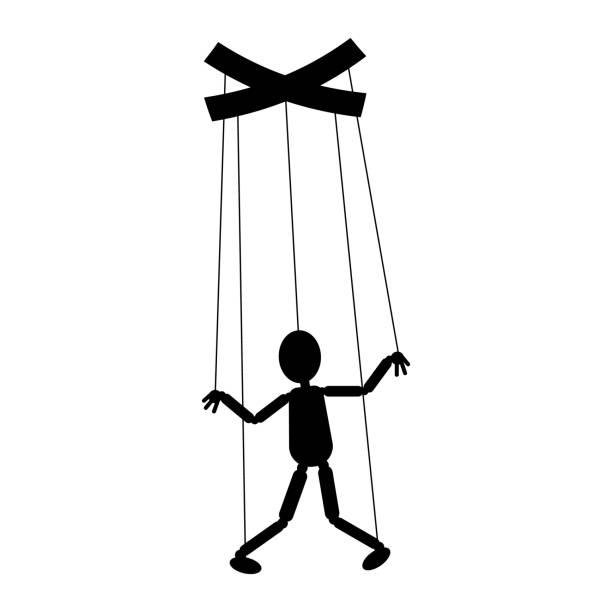
\includegraphics[scale=0.5]{Figures/marionette.jpg}}
  \\
  {\text{QObj1}}
  \end{tabular}
  }&{}&{
  \begin{tabular}{c}
  {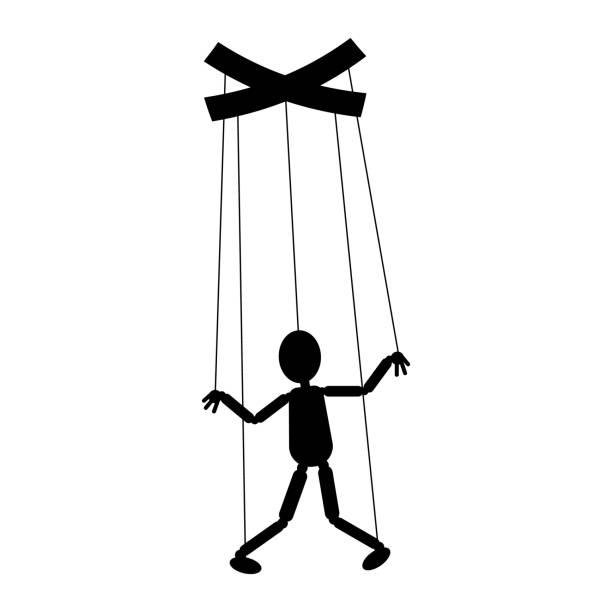
\includegraphics[scale=0.5]{Figures/marionette.jpg}}
  \\
  {\text{QObj2}}
  \end{tabular}
  }&{}&{
  \begin{tabular}{c}
  {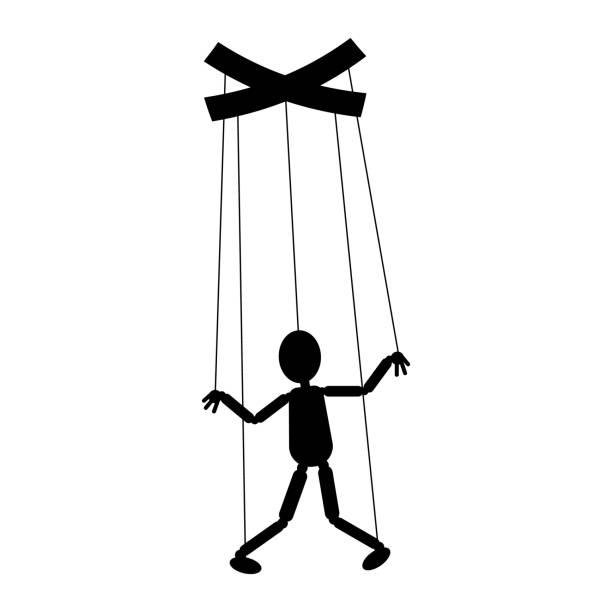
\includegraphics[scale=0.5]{Figures/marionette.jpg}}
  \\
  {\text{QObj3}}
  \end{tabular}
  }\\
  {
  \begin{tabular}{c}
  qApp\\
  Qt mail box\\
  \begin{tabular}{|c|c|c|}
  \hline
  {}&{}&{}\\
  \hline
  \end{tabular}\\
  {\textbf{Thread}}
  \end{tabular}
  }
  \ar@(r,r)[u]
  \ar@(r,d)[rru]
  \ar@(r,d)[rrrru]
  &{}&{}&{}&{
  {\textbf{OS}}
  }
  \ar@{-->}[llll]
  \\
}
\]
Так же для полноты картины давайте я приведу пример event loop в Qt экосистеме.
\begin{cppcode}
int main(int argc, char* argv[]) {
  QApplication QRunTime(argc, argv);
  Application application;
  QRunTime.exec();
  return 0;
}
\end{cppcode}
Вторая строчка создает Qt экосистему для данного thread-а.
Третья строчка создает объект приложения.
Важно, что его компоненты будут взаимодействовать с Qt экосистемой.
В этой строчке само приложение просто положили в память, корректно инициализировали и корректно подключили к Qt экосистеме.
И четвертая строчка запускает event loop.
Именно в этой функции крутится цикл, который выполняет всю работу.
В частности внутри этого цикла и будет выполняться работа при получении сообщения адресатом.

Функционирование Qt экосистемы можно представлять себе следующим образом:
\begin{center}
\begin{tabular}{rr}
{
1)\quad\scalebox{0.5}{
\boxed{
\begin{minipage}[\baselineskip]{12cm}
\[
\xymatrix@C=15pt{
  {}&{
  \begin{matrix}
  {\verb"QApplication"}\\
  {
  \begin{array}{|c|c|c|c|}
  \hline
  {\text{\color{red}\Letter}}&{\text{\Letter}}&{\ldots}&{\text{\Letter}}\\
  \hline
  \end{array}
  }
  %\ar@(l,u)[ld]
  %\ar@{<-}@(r,u)[rrdd]+(4,4)|-{\verb"postEvent"}
  \end{matrix}
  }&{}&{}\\
  {\phantom{\text{\Letter}}}
  %\ar[d]|-{\verb"event"}
  %\ar[dr]+(-4,15)|-{\verb"event"}
  %\ar[drrr]+(-4,15)|-{\verb"event"}&{}&{}&{}
  \\
  {
  \begin{matrix}
  {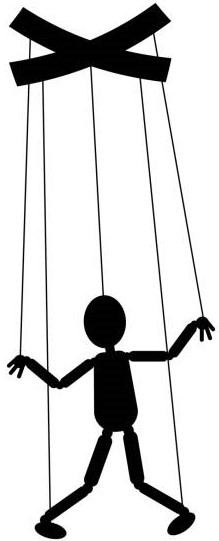
\includegraphics[scale=0.5]{Figures/marionette1.jpg}}\\
  {\verb"QObject1"}
  \end{matrix}
  }&{
  \begin{matrix}
  {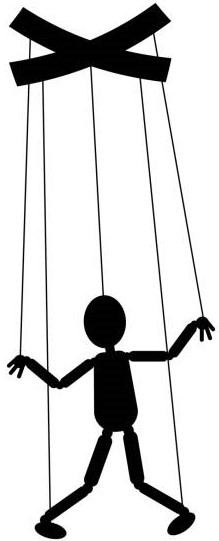
\includegraphics[scale=0.5]{Figures/marionette1.jpg}}\\
  {\verb"QObject2"}
  \end{matrix}
  }&{
  \begin{matrix}
  {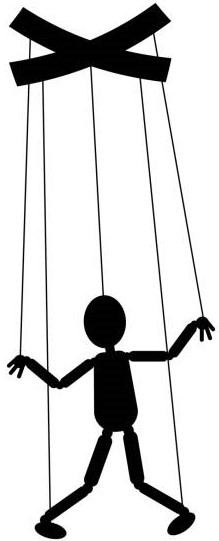
\includegraphics[scale=0.5]{Figures/marionette1.jpg}}\\
  {\verb"QObject3"}
  \end{matrix}
  }&{
  \begin{matrix}
  {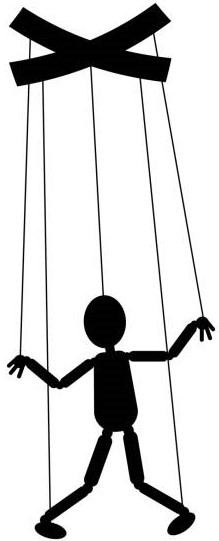
\includegraphics[scale=0.5]{Figures/marionette1.jpg}}\\
  {\verb"QObject4"}
  \end{matrix}
  }\\
}
\]
\end{minipage}
}}
}&{
5)\quad\scalebox{0.5}{
\boxed{
\begin{minipage}[\baselineskip]{12cm}
\[
\xymatrix@C=15pt{
  {}&{
  \begin{matrix}
  {\verb"QApplication"}\\
  {
  \begin{array}{|c|c|c|c|}
  \hline
  {\phantom{\text{\Letter}}}&{\text{\Letter}}&{\ldots}&{\text{\Letter}}\\
  \hline
  \end{array}
  }
  %\ar@(l,u)[ld]
  %\ar@{<-}@(r,u)[rrdd]+(4,4)|-{\verb"postEvent"}
  \end{matrix}
  }&{}&{}\\
  {{\text{\Letter}}}
  %\ar@[red][d]|-{\verb"event"}
  %\ar@[red][dr]+(-4,15)|-{\verb"event"}
  \ar@[red][drrr]+(-4,15)|-{\verb"event"}&{}&{}&{}
  \\
  {
  \begin{matrix}
  {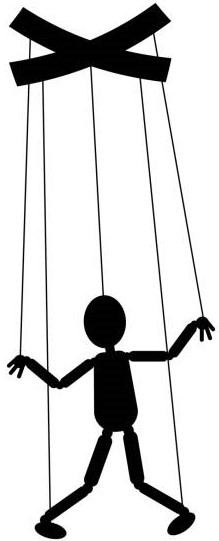
\includegraphics[scale=0.5]{Figures/marionette1.jpg}}\\
  {\verb"QObject1"}
  \end{matrix}
  }&{
  \begin{matrix}
  {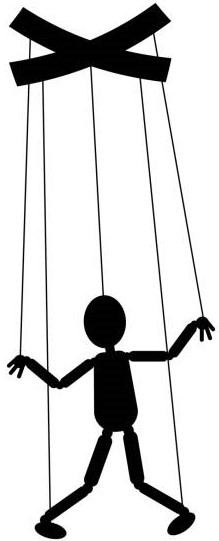
\includegraphics[scale=0.5]{Figures/marionette1.jpg}}\\
  {\verb"QObject2"}
  \end{matrix}
  }&{
  \begin{matrix}
  {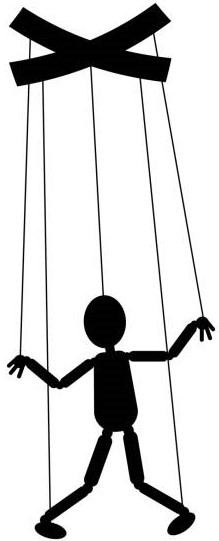
\includegraphics[scale=0.5]{Figures/marionette1.jpg}}\\
  {\verb"QObject3"}
  \end{matrix}
  }&{
  \begin{matrix}
  {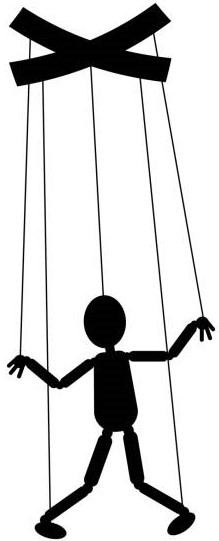
\includegraphics[scale=0.5]{Figures/marionette1.jpg}}\\
  {\verb"QObject4"}
  \end{matrix}
  }\\
}
\]
\end{minipage}
}}
}\\
{
2)\quad\scalebox{0.5}{
\boxed{
\begin{minipage}[\baselineskip]{12cm}
\[
\xymatrix@C=15pt{
  {}&{
  \begin{matrix}
  {\verb"QApplication"}\\
  {
  \begin{array}{|c|c|c|c|}
  \hline
  {\phantom{\text{\Letter}}}&{\text{\Letter}}&{\ldots}&{\text{\Letter}}\\
  \hline
  \end{array}
  }
  \ar@(l,u)[ld]
  %\ar@{<-}@(r,u)[rrdd]+(4,4)|-{\verb"postEvent"}
  \end{matrix}
  }&{}&{}\\
  {{\text{\color{red}\Letter}}}
  %\ar[d]|-{\verb"event"}
  %\ar[dr]+(-4,15)|-{\verb"event"}
  %\ar[drrr]+(-4,15)|-{\verb"event"}&{}&{}&{}
  \\
  {
  \begin{matrix}
  {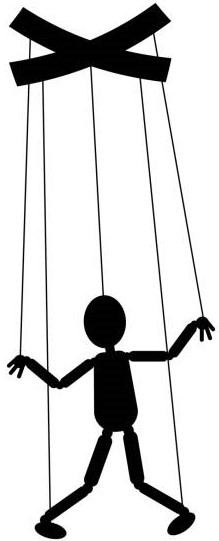
\includegraphics[scale=0.5]{Figures/marionette1.jpg}}\\
  {\verb"QObject1"}
  \end{matrix}
  }&{
  \begin{matrix}
  {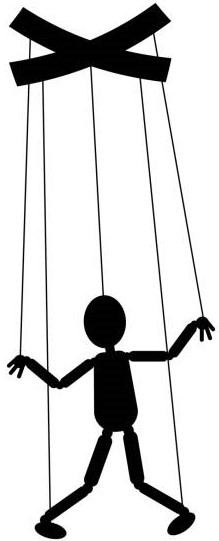
\includegraphics[scale=0.5]{Figures/marionette1.jpg}}\\
  {\verb"QObject2"}
  \end{matrix}
  }&{
  \begin{matrix}
  {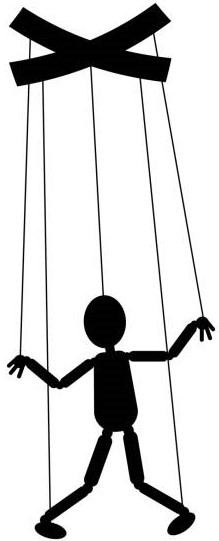
\includegraphics[scale=0.5]{Figures/marionette1.jpg}}\\
  {\verb"QObject3"}
  \end{matrix}
  }&{
  \begin{matrix}
  {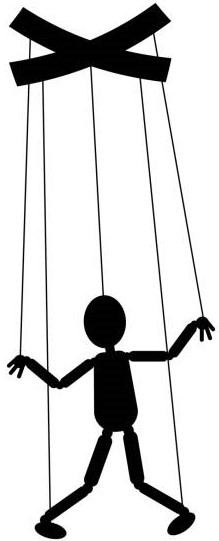
\includegraphics[scale=0.5]{Figures/marionette1.jpg}}\\
  {\verb"QObject4"}
  \end{matrix}
  }\\
}
\]
\end{minipage}
}}
}&{
6)\quad\scalebox{0.5}{
\boxed{
\begin{minipage}[\baselineskip]{12cm}
\[
\xymatrix@C=15pt{
  {}&{
  \begin{matrix}
  {\verb"QApplication"}\\
  {
  \begin{array}{|c|c|c|c|}
  \hline
  {\phantom{\text{\Letter}}}&{\text{\Letter}}&{\ldots}&{\text{\Letter}}\\
  \hline
  \end{array}
  }
  %\ar@(l,u)[ld]
  \ar@{<-}@(r,u)@[red][rrdd]+(4,4)|-{\verb"postEvent"}
  \end{matrix}
  }&{}&{}\\
  {{\text{\Letter}}}
  %\ar@[red][d]|-{\verb"event"}
  %\ar@[red][dr]+(-4,15)|-{\verb"event"}
  \ar[drrr]+(-4,15)|-{\verb"event"}&{}&{}&{}
  \\
  {
  \begin{matrix}
  {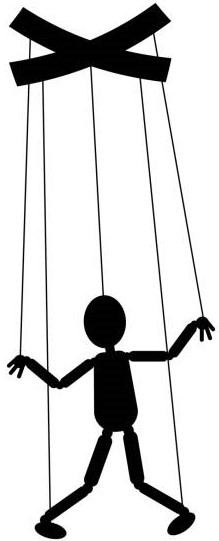
\includegraphics[scale=0.5]{Figures/marionette1.jpg}}\\
  {\verb"QObject1"}
  \end{matrix}
  }&{
  \begin{matrix}
  {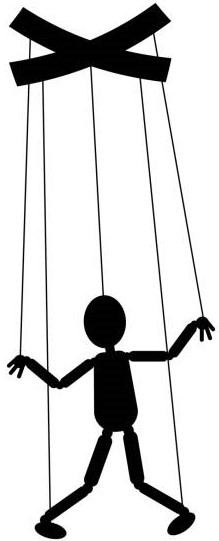
\includegraphics[scale=0.5]{Figures/marionette1.jpg}}\\
  {\verb"QObject2"}
  \end{matrix}
  }&{
  \begin{matrix}
  {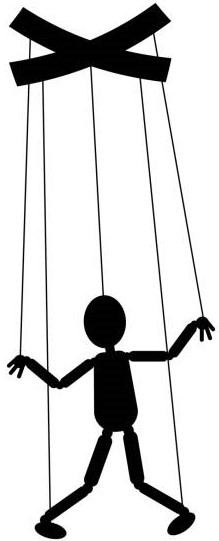
\includegraphics[scale=0.5]{Figures/marionette1.jpg}}\\
  {\verb"QObject3"}
  \end{matrix}
  }&{
  \begin{matrix}
  {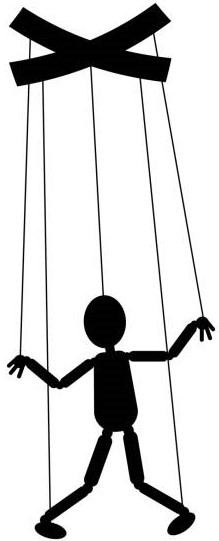
\includegraphics[scale=0.5]{Figures/marionette1.jpg}}\\
  {\verb"QObject4"}
  \end{matrix}
  }\\
}
\]
\end{minipage}
}}
}\\
{
3)\quad\scalebox{0.5}{
\boxed{
\begin{minipage}[\baselineskip]{12cm}
\[
\xymatrix@C=15pt{
  {}&{
  \begin{matrix}
  {\verb"QApplication"}\\
  {
  \begin{array}{|c|c|c|c|}
  \hline
  {\phantom{\text{\Letter}}}&{\text{\Letter}}&{\ldots}&{\text{\Letter}}\\
  \hline
  \end{array}
  }
  %\ar@(l,u)[ld]
  %\ar@{<-}@(r,u)[rrdd]+(4,4)|-{\verb"postEvent"}
  \end{matrix}
  }&{}&{}\\
  {{\text{\Letter}}}
  \ar@[red][d]|-{\verb"event"}
  %\ar[dr]+(-4,15)|-{\verb"event"}
  %\ar[drrr]+(-4,15)|-{\verb"event"}&{}&{}&{}
  \\
  {
  \begin{matrix}
  {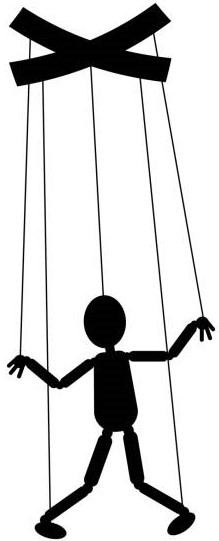
\includegraphics[scale=0.5]{Figures/marionette1.jpg}}\\
  {\verb"QObject1"}
  \end{matrix}
  }&{
  \begin{matrix}
  {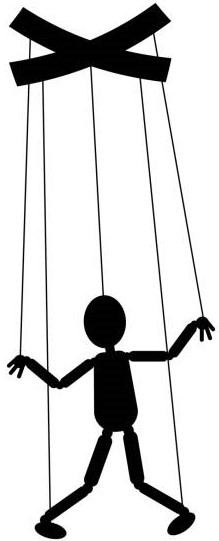
\includegraphics[scale=0.5]{Figures/marionette1.jpg}}\\
  {\verb"QObject2"}
  \end{matrix}
  }&{
  \begin{matrix}
  {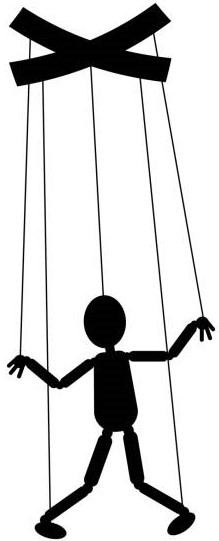
\includegraphics[scale=0.5]{Figures/marionette1.jpg}}\\
  {\verb"QObject3"}
  \end{matrix}
  }&{
  \begin{matrix}
  {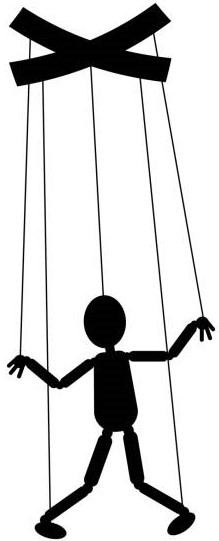
\includegraphics[scale=0.5]{Figures/marionette1.jpg}}\\
  {\verb"QObject4"}
  \end{matrix}
  }\\
}
\]
\end{minipage}
}}
}&{
7)\quad\scalebox{0.5}{
\boxed{
\begin{minipage}[\baselineskip]{12cm}
\[
\xymatrix@C=15pt{
  {}&{
  \begin{matrix}
  {\verb"QApplication"}\\
  {
  \begin{array}{|c|c|c|c|}
  \hline
  {{\text{\Letter}}}&{\text{\Letter}}&{\ldots}&{\text{\color{red}\Letter}}\\
  \hline
  \end{array}
  }
  %\ar@(l,u)[ld]
  \ar@{<-}@(r,u)[rrdd]+(4,4)|-{\verb"postEvent"}
  \end{matrix}
  }&{}&{}\\
  {{\text{\Letter}}}
  %\ar@[red][d]|-{\verb"event"}
  %\ar@[red][dr]+(-4,15)|-{\verb"event"}
  \ar[drrr]+(-4,15)|-{\verb"event"}&{}&{}&{}
  \\
  {
  \begin{matrix}
  {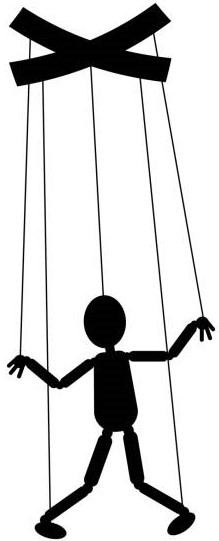
\includegraphics[scale=0.5]{Figures/marionette1.jpg}}\\
  {\verb"QObject1"}
  \end{matrix}
  }&{
  \begin{matrix}
  {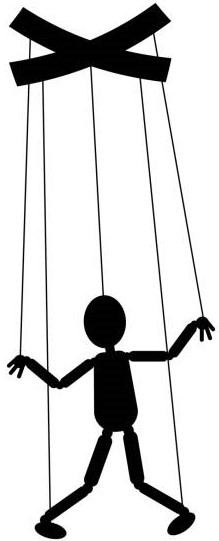
\includegraphics[scale=0.5]{Figures/marionette1.jpg}}\\
  {\verb"QObject2"}
  \end{matrix}
  }&{
  \begin{matrix}
  {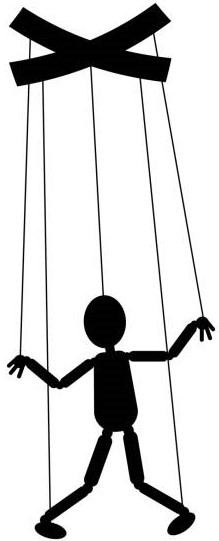
\includegraphics[scale=0.5]{Figures/marionette1.jpg}}\\
  {\verb"QObject3"}
  \end{matrix}
  }&{
  \begin{matrix}
  {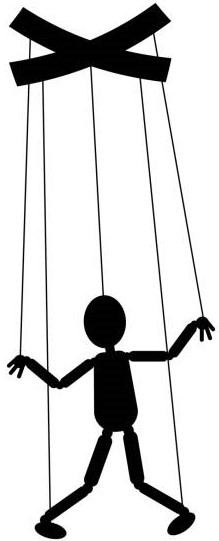
\includegraphics[scale=0.5]{Figures/marionette1.jpg}}\\
  {\verb"QObject4"}
  \end{matrix}
  }\\
}
\]
\end{minipage}
}}
}\\
{
4)\quad\scalebox{0.5}{
\boxed{
\begin{minipage}[\baselineskip]{12cm}
\[
\xymatrix@C=15pt{
  {}&{
  \begin{matrix}
  {\verb"QApplication"}\\
  {
  \begin{array}{|c|c|c|c|}
  \hline
  {\phantom{\text{\Letter}}}&{\text{\Letter}}&{\ldots}&{\text{\Letter}}\\
  \hline
  \end{array}
  }
  %\ar@(l,u)[ld]
  %\ar@{<-}@(r,u)[rrdd]+(4,4)|-{\verb"postEvent"}
  \end{matrix}
  }&{}&{}\\
  {{\text{\Letter}}}
  %\ar@[red][d]|-{\verb"event"}
  \ar@[red][dr]+(-4,15)|-{\verb"event"}
  %\ar[drrr]+(-4,15)|-{\verb"event"}&{}&{}&{}
  \\
  {
  \begin{matrix}
  {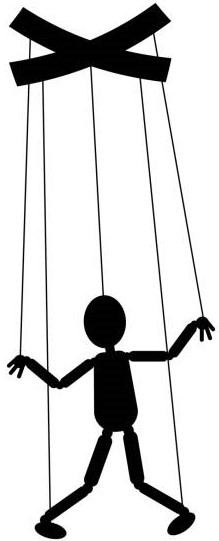
\includegraphics[scale=0.5]{Figures/marionette1.jpg}}\\
  {\verb"QObject1"}
  \end{matrix}
  }&{
  \begin{matrix}
  {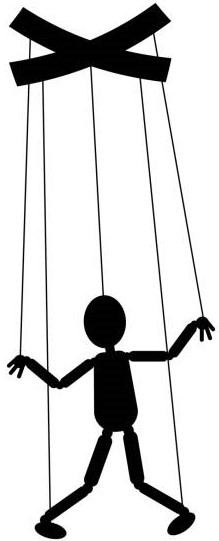
\includegraphics[scale=0.5]{Figures/marionette1.jpg}}\\
  {\verb"QObject2"}
  \end{matrix}
  }&{
  \begin{matrix}
  {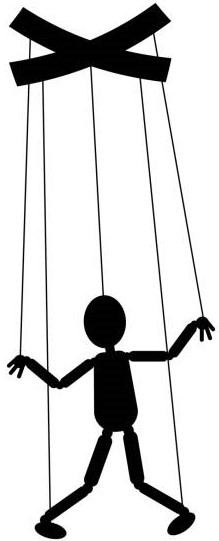
\includegraphics[scale=0.5]{Figures/marionette1.jpg}}\\
  {\verb"QObject3"}
  \end{matrix}
  }&{
  \begin{matrix}
  {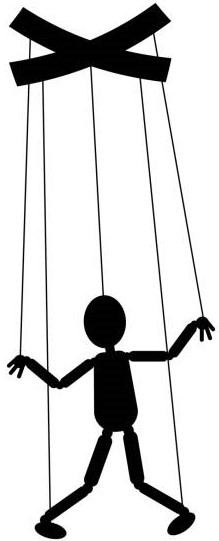
\includegraphics[scale=0.5]{Figures/marionette1.jpg}}\\
  {\verb"QObject4"}
  \end{matrix}
  }\\
}
\]
\end{minipage}
}}
}&{
}\\
\end{tabular}
\end{center}
Прокомментируем поведение системы выше:
\begin{enumerate}
\item \verb"QApplication" проверяет пуст ли почтовый ящик или нет.
Если почтовый ящик пуст, то система засыпает пока не появятся сообщения от операционной системы.
Эти сообщения будут трансформированы в Qt сообщения и сложены в почтовый ящик.

\item Если почтовый ящик не пуст, то вынимаем первое сообщение из ящика.
Теперь можно совершать доставку сообщения адресатам

\item В Qt экосистеме обработчик сообщения у адресата -- функция \verb"event".
Вызываем эту функцию для \verb"QObject1" и передаем в нее текущее сообщение.

\item Теперь вызываем \verb"event" у \verb"QObject2" и передаем в нее текущее сообщение.

\item На этом шаге вызываем \verb"event" у \verb"QObject4" и передаем в нее текущее сообщение.

\item В результате обработки сообщения \verb"QObject4" сформировал сообщение и отправляет его в почтовый ящик \verb"QApplication".

\item Сообщение от \verb"QObject4" положили в конец очереди в почтовый ящик.
На этом одна итерация event loop-а завершается и весь процесс повторяется с самого начала.
\end{enumerate}


\subsubsection{Идея имплементации}

Я уже приводил пример event loop-а для двух Message Driven System.
Давайте я в общих чертах скажу, как строится произвольная такая система.
Прежде всего у нас должен почтовый ящик и event loop, которые выглядят как-то так.
\begin{cppcode}
MailBox gBox;

int main() {
  Event e;
  while(getEvent(&e)) {
    dispatchEvent(e);
  }
  return 0;
}
\end{cppcode}
Тут важно понимать, что почтовый ящик является глобальным ресурсом для данного thread-а.
Как мы видим весь event loop устроен очень просто, мы вынимаем сообщение из почтового ящика в функции \verb"getEvent".
А потом запускаем доставку сообщений в методе \verb"dispatchEvent".
При такой имплементации цикл заканчивается, если \verb"getEvent" вернет \verb"false".
В этой имплементации отсутствует код, перерабатывающий сообщения операционной системы в сообщения экосистемы.

Функция доставки сообщений работает приблизительно так
\begin{cppcode}
void dispatchEvent(const Event& e) {
  for (auto obj : addresseesOf(e)) {
    obj->handleEvent(e);
  }
}
\end{cppcode}
То есть для каждого сообщения составляется список его адресатов, а потом мы просто зовем служебную функцию \verb"handleEvent" у всех адресатов блокирующим образом.

Теперь, что из себя представляет сообщение?
Обычно это данные и некоторая метаинформация, которая помогает понять, что это за данные.
Ведь передавать мы должны уметь все что угодно.
Кратко можно думать про это так
\begin{cppcode}
enum class EventType {
  Mouse,
  Keyboard,
  /* ... */};

class Event {
public:
  /*Constructor*/
  EventType type() const;
  const void* data() const;
  
private:
  EventType type_;
  std::any data_;
};
\end{cppcode}
Здесь \verb"EventType" -- это заранее известный набор констант для всех возможных типов сообщений.
Многие системы имеют выделенный диапазон типов для создания пользовательских сообщений.
Само сообщение содержит информацию о типе и данные.
Я использую \verb"std::any" как стирающий тип, который умеет хранить что угодно.

Теперь перейдем к обработке сообщений.
Для хранения списка адресатов, который используется в функции \verb"dispatchEvent" можно использовать интерфейсы или стирающие ссылки.
\begin{cppcode}
std::vector<EventHandler> addresseesOf(const Event& e)
\end{cppcode}
здесь \verb"EventHandler" -- это стирающий указатель на объект, которому доставляется сообщение.
Для попадания в этот список в системе должны быть свои механизмы, которые я тут не собираюсь обсуждать.
Теперь обработка сообщений выглядит как-то так
\begin{cppcode}
class Obj1 {
public:
  void handleEvent(const Event& e) override {
    switch(e.type()) {
      case EventType::Mouse:
        MouseEvent& Data = cast<MouseEvent&>(e.data());
        // handle mouse event
      break;
      case EventType::Keyboard:
        KeyboardEvent& Data = cast<KeyboardEvent&>(e.data());
        // handle keyboard event
      break;
      ...
    }
  }
};
\end{cppcode}
Каждый объект должен прочитать тип сообщения, а потом в зависимости от этой информации вынуть нужные данные и отреагировать на них.
Возможно, что \verb"handleEvent" игнорирует какие-то сообщения, а может быть даже и все.
Функция \verb"cast" выше -- это псевдокод, который призван показать, что мы вынимаем из сообщения данные, которые там зашифрованы в зависимости от информации о типе сообщения.

\subsubsection{Неблокирующие операции}
% TO DO

Теперь, если мы орудуем в рамках Message Driven System, у нас есть два способа отправить данные из одной функции в другую.
\begin{enumerate}
\item Прямой блокирующий вызов.
Этот случай -- это просто обычный вызов функции внутри другой функции.
Например, если работает обработчик сообщений \verb"Obj1", то он может дернуть (если знает адрес) какой-нибудь метод из \verb"Obj2".
В этом случае реакция на данные происходит немедленно.

\item Посылка сообщения.
В этом случае если обработчик сообщений \verb"Obj1" произвел какие-то данные для \verb"Obj2", то он не вызывает метод \verb"Obj2".
Вместо этого он создает сообщение, куда складывает эту информацию, пишет в качестве адресата \verb"Obj2" на конверте и складывает письмо в почтовый ящик.
В этом случае реакция на сообщение произойдет не сразу же во время отправки сообщения, а позже, когда экосистема дойдет до обработки сообщения и передаст его адресату.
Такое поведение называется неблокирующим вызовом.
Это поведение важно держать в голове, потому что важно поместить в сообщение все данные, чтобы они были живы, когда сообщение дойдет до адресата.
Нельзя вкладывать ссылки и указатели на локальные данные, просто потому что они все умрут к моменту передачи сообщения по назначению.
\end{enumerate}
Второй подход нужен для того, чтобы не блокировать на долго одной задачей ядро процессора.
Чтобы на одном ядре успевали покрутиться разные обработчики сообщений.
Это делается для того, чтобы GUI был отзывчивым и окна не подвисали.
В рамках такой экосистемы полезно иметь неблокирующий observer pattern, в котором observable не сразу дергает методы \verb"onSubscribe" и \verb"onNotify", а посылает сообщения через Message Driven System.

\subsection{Неблокирующий Observer Pattern}
\label{section::ObserverNonBlocking}

\subsubsection{Общая схема}

Для неблокирующего observer pattern нам прежде всего нужна некоторая Message Driven System, которая будет использоваться для пересылки сообщений.
Грубо общую модель можно описать следующей диаграммой.

\[
\xymatrix{
  {\vphantom{\text{Message System}}}
    {\save
  [].[rr]*+[F--]\frm{}
  \restore
  }  
  &{\text{Message System}}\ar[rd]\ar[rdd]&{}\\
  {\text{Observable}}\ar[ru]<-0.5em>\ar[ru]&{}&{\text{Observer0}}\\
  {}&{}&{\text{Observer1}}\\
}
\]
В рамках такой системы \verb"Observable" не дергает методы \verb"Observer" напрямую.
Вместо этого он посылает данные в виде сообщения каждому \verb"Observer"-у.
Давайте отметим несколько интересных изменений, которые возникают из-за такой системы.
\begin{itemize}
\item Прежде всего, нужен механизм адресации для того, чтобы можно было отправлять сообщения конкретным объектам.
Обычно в любой Message Driven System такая возможность имеется из коробки и тут не надо ничего изобретать.

\item В зависимости от возможностей Message Driven System-ы бывает нужно уметь проверять жив ли объект, которому отправляется сообщение.
Причем жив ли он не в момент отправки, а в момент доставки сообщения.
Например в системе Qt таких гарантий нет.

\item Так как сообщения посылаются разными сообщениями каждый своему адресату, то не возможно пересылать данные по ссылке.
Приходится в каждое сообщение от \verb"Observable" вкладывать копию данных, которые надо пересылать.

\item Когда же сообщение доставляется \verb"Observer", то мы гарантируем, что получатель ровно один и больше сообщение не понадобится.
В этом случае данные можно безболезненно вынуть (мувнуть) из сообщения.

\item Обратите внимание, что общение между \verb"Observer" и \verb"Observable" теперь происходит не мгновенно блокирующим образом, а с задержками.
Они не реагируют друг на друга мгновенно.
В этом случае можно думать, что общение портов происходит как бы через сеть.
А все сетевое взаимодействие принято описывать с помощью State Machine.
\end{itemize}
Важно помнить, что конкретная имплементация зависит от выбора Message Driven System, от ее возможностей и предоставляемых гарантий.

\subsubsection{Передача данных поверх Qt}

\paragraph{Дефекты Qt}

Начать я хочу с важного замечания по поводу системы Qt.
Когда \verb"QApplication" доставляет сообщения адресатам
\[
\xymatrix{
  {\verb"QApplication"}\ar[rr]^{\verb"event"}&{}&{\verb"QObject"}\\
}
\]
он дергает блокирующим образом метод \verb"event" по адресу объекта получателя.
Однако, нет никаких гарантий, что объект, у которого мы дергаем \verb"event" еще жив.
Вокруг этой проблемы есть огромное количество костылей в Qt, включая отложенное удаление объекта.
Получается, что в Qt экосистеме нельзя просто так слать сообщение \verb"QObject" напрямую.
Нужно перед дерганьем метода \verb"event" проверить жив ли объект.
И в Qt есть специальный следящий указатель (который по сути является другой имплементацией следящего указателя из раздела~\ref{section::TrackingPtr}) и называется он \verb"QPointer".
Так же важно, что объект \verb"QApplication" всегда жив (на основном thread-е конечно).
Тогда правильная схема -- отправить сначала сообщение \verb"QApplication" на своем thread-е.
Если получатель живет на этом же thread-е, то \verb"QApplication" в начале проверяет жив ли адресат и после этого дергает у него \verb"event".
Если же нужно послать сообщение другому thread-у, то тут надо огранизовывать взаимодействие между \verb"QApplication" на разных thread-ах.
Благо Qt дает некую поддержку из коробки для этого.
Но я не хочу это обсуждать.

\paragraph{QPort}

Обратите внимание, что сейчас обсуждается задача безопасной пересылки сообщения в экосистеме Qt.
Этой проблемы может не быть в других экосистемах, но так и хорошо, я смогу продемонстрировать как подобные вещи решаются.
Так как это задача более низкоуровневая, чем observer pattern, то здесь речь будет идти о более простом примитиве, который я хочу назвать \verb"QPort".
Его задача будет состоять лишь в том, чтобы уметь передавать безопасно данные из от одного порта к другому не блокирующим образом.
Ничего другого эти порты уметь не будут.
И уже поверх этих портов мы построим observer pattern.
Давайте схематично изобразим, что из себя представляет сообщение и как оно передается.
\[
\xymatrix@R=15pt{
  {}&{}&{\verb"QApplication"}
  \ar@{=>}@(r,u)[rdd]^{2}
  &{}
  \\
  {}&{{\verb"Message"}}
  \ar@{=>}@(u,l)[ur]^{1}
  {\save
  [].[ddd]*+[F-]\frm{}
  \restore
  }
  &{}&{}\\
  {{\verb"QPort"}}&
  {{\verb"QPtr from"}}
  \ar[l]
  {\save
  [].[dd]*[F-]\frm{}
  \restore
  }
  &{}&{\verb"QPort"}\\
  {}&{{\verb"QPtr to"}}
  \ar[rru]
  &{}&{}\\
  {}&{{\verb"any data"}}&{}&{}\\
}
\]
\begin{enumerate}
\item Сообщение \verb"Message" содержит три поля
\begin{enumerate}
\item Адрес порта отправителя в виде \verb"QPointer".
Адрес отправителя нам понадобится для двусторонней коммуникации в observer pattern.

\item Адрес порта получателя в виде \verb"QPointer".

\item И сами данные в виде стирающего типа \verb"std::any".
Это означает, что пользователь портов должен знать, что он отправляет и написать весь функционал поддерживающий типизацию поверх этой системы.
\end{enumerate}
Тут надо сказать зачем данные отправляются в виде \verb"std::any".
Почему мы не используем шаблонный порт \verb"QPort<T>", что гарантировало бы доставку сообщений определенного типа.
Тут к сожалению выстреливает еще одна особенность именно экосистемы Qt.
Дело в том, что для правильной работы Qt выполняет генерацию кода для каждого \verb"QObject".
Для этого есть специальный метакомпилятор \verb"moc".
И метакомпилятор всегда применяется к \verb"cpp" файлам и никогда не применяется к хедерам.
Но шаблон нельзя разделить на хедер и сурс.
Потому приходится обходиться без шаблонов с помощью стирающих типов.

\item Порт отправитель не шлет сообщение напрямую порту получателю, вместо этого сообщение отправляется \verb"QApplication" по стрелке (1).
Это действие всегда безопасно, потому что Qt экосистема гарантируется, что \verb"QApplication" будет жить, если жив на данном thread-е дольше всех остальных объектов.
Он создается первым, и удаляется последним.
Межthread-овая коммуникация требует некоторой отдельной работы.

\item Теперь нам надо будет внести модификацию в поведение \verb"QApplication", чтобы он умел переотправлять наши сообщения порту получателю.
Идея в том, что в начале \verb"QApplication" проверяет \verb"QPointer" получателя.
Так как получатель живет на этом же thread-е, то у нас нет гонки между деструктором получателя и обработкой сообщения.
Либо одно либо другое происходит раньше.
Потому \verb"QApplication" может спокойно проверить \verb"QPointer" и если он не \verb"nullptr", то можно дернуть по его адресу метод \verb"event".
\end{enumerate}

\paragraph{Сообщения}
% TO DO

Все сообщения в Qt экосистеме должны быть унаследованы публично от \verb"QEvent".
Как было изображено на диаграмме мы должны иметь
\begin{cppcode}
class Message : public QEvent {
public:
  using CPointer = QPointer<QEvent>;
  ...
private:
  CPointer from_;
  CPointer to_;
  std::any data_;
};
\end{cppcode}
Кроме того, у каждого сообщения есть идентификатор \verb"QEvent::Type", который представляет из себя целое число.
Это просто тег, который говорит получателю, что это за сообщения, чтобы потом суметь вынуть данные.
Экосистема Qt позволяет зарегистрировать автоматически первый свободный идентификатор.
Для этого выделим статический метод, который зарегистрирует тип при первом вызове и будет возвращать его значение всюду далее.
\begin{cppcode}
class Message : public QEvent {
public:
  static QEvent::Type type() {
    static int message_type = registerEventType();
    return QEvent::Type{message_type};
  }
  ...
private:
  ...
};
\end{cppcode}
Напишем полностью интерфейс класса
\begin{cppcode}
class Message : public QEvent {
public:
  using CPointer = QPointer<QObject>;
  static QEvent::Type type();
  
  Message(CPointer from, CPointer to, const std::any& data);
  Message(CPointer from, CPointer to, std::any&& data);
  
  std::any&& extract();
  
  bool isReceiverAlive() const;
  
  CPointer receiver() const;
  CPointer to() const;
  CPointer from() const;
private:
  CPointer from_;
  CPointer to_;
  std::any data_;
};
\end{cppcode}
В начале покажем, как нужно написать конструкторы
\begin{cppcode}
Message(CPointer from, CPointer to, const std::any& data)
  : QEvent(type()), from_(std::move(from)), to_(std::move(to)),
    data_(data) {}
Message(CPointer from, CPointer to, std::any&& data)
  : QEvent(type()), from_(std::move(from)), to_(std::move(to)),
    data_(std::move(data)) {}
\end{cppcode}
Тут все просто, мы вызываем базовый конструктор, в который передаем тип сообщения вызывая статическую функцию \verb"type".
Нам нужны два конструктора, чтобы была возможность положить новые данные в сообщения или мувнуть туда уже существующие.
Теперь имплементация оставшихся методов
\begin{cppcode}
class Message : public QEvent {
public:
  ...
  std::any&& extract() {
    return std::move(data_);
  }
  bool isReceiverAlive() const {
    return to_;
  }
  CPointer receiver() const {
    return to_;
  }
  CPointer to() const {
    return to_;
  }
  CPointer from() const {
    return from_;
  }
private:
  ...
};
\end{cppcode}
Тут все просто кроме быть может метода \verb"extract".
Дело в том, что когда сообщение приходит в порт назначения, то оно больше использоваться не будет.
А значит, нам надо вынуть данные из сообщения.
Для этого нужно мувнуть данные наружу.
Тут есть две опции:
\begin{enumerate}
\item Вернуть \verb"std::any&&".

\item Вернуть \verb"std::any".
\end{enumerate}
Но в любом случае нужно будет вокруг \verb"data_" добавить \verb"std::move(data_)".
Это чуть ли ни единственный пример, когда нужно писать \verb"std::move" в \verb"return".
Без этого каста, будет сниматься копия с данных во второй имплементации.
А первая имплементация выдаст ошибку компиляции.

\paragraph{Имплементация QPort}

Начнем с интерфейса
\begin{cppcode}
class QPort : public QObject {
  Q_OBJECT
public:
  using Message = detail::Message;
  using CPointer = Message::CPointer;

  void send(CPointer from, CPointer to, std::any data) const;
  bool event(QEvent* event) override;

protected:
  virtual void action(CPointer from, std::any&& data) = 0;

private:
  static constexpr bool k_is_processed = true;
};
\end{cppcode}
Давайте прокомментируем, что тут происходит.
Прежде всего, чтобы быть участником Qt экосистемы и уметь получать сообщения от системы нужно публично унаследоваться от \verb"QObject".
Однако, этого мало.
Из-за кодогенерации, нужно для каждого такого участника экосистемы сгенерировать некоторые служебные данные, без которых взаимодействие с системой не возможно.
Для этого служит макрос \verb"Q_OBJECT", который добавляется сразу же в приватную часть класса.

Обратите внимание, что я страшный сторонник type erasure и ненавистник наследования с виртуальными методами внезапно начинаю использовать виртуальные методы.
Связано это с тем, что в основе дизайна Qt лежит возможность наследоваться от базового класса, модифицируя его поведение переопределением виртуальных методов.
Если фреймворк использует такой подход, то использовать стирающие типы будет очень сложно, код будет менее читаемым и громоздским и скорее всего еще и будет менее эффективным.
Потому раз этот фреймворк использует такой подход, то нужно придерживаться его при взаимодействии с этим фреймворком.
Но вот снаружи я могу использовать любые парадигмы, которые захочу.

Метода \verb"action" является чисто виртуальным.
Это действие, которое будет выполняться при получении сообщения.
Обратите внимание, что данные получаются по rvalue ссылке, что означает, что мы будем вынимать данные из сообщения и передавать в этот метод через мув.
Этот метод должен быть перегружен у наследника, какими будут \verb"Observable" и \verb"Observer".

Теперь как имплементируется метод отправки сообщения
\begin{cppcode}
void QPort::send(CPointer from, CPointer to, std::any data) const {
  QCoreApplication::postEvent(
      QCoreApplication::instance(), // to whom
      new Message(std::move(from), std::move(to), std::move(data)));
}
\end{cppcode}
Тут надо обратить внимание на то, что внутри вызывается всего лишь одна функция Qt экосистемы \verb"postEvent", которая просто помещает сообщение в почтовый ящик.
Эта функция принимает два аргумента:
\begin{enumerate}
\item Адрес получателя, как адрес объекта.
Здесь мы пишем адрес текущего \verb"QApplication".
Этот объект обеспечивает существование и функционирование Qt экосистемы на данном thread-е и потому ему письмо всегда можно доставить безопасно.

\item Сообщение передаваемый по указателю.
Сообщение обязано быть унаследовано от \verb"QEvent".
Пусть вас не смущает голое \verb"new" в коде.
Данная функция захватывает владение сообщением и гарантирует его корректный менеджмент.
При работе Qt всегда приходится думать кто кем владеет, чтобы случайно не было утечек данных.
\end{enumerate}

И в теперь надо обсудить обработку входящих сообщений портом в функции \verb"event":
\begin{cppcode}
static constexpr bool k_is_processed = true;

bool QPort::event(QEvent* event) {
  if (event->type() == Message::type()) {
    Message* msg = static_cast<Message*>(event);
    action(msg->from(), msg->extract());
    return k_is_processed;
  }
  return QObject::event(event);
}
\end{cppcode}
Все что тут происходит мы смотрим на получаемое сообщение и если оно нужного нам типа, то мы вынимаем из него данные и уже скармливаем эти данные функции \verb"action", которую мы обсудили выше.

\paragraph{Поддержка сообщений со стороны Qt}

На самом деле, чтобы эта схема работала нужно еще внести дополнительные изменения в \verb"QApplication", чтобы он знал, как реагировать на наши сообщения.
Это тоже делается наследованием от \verb"QApplication".
Все что мы сделаем -- добавим правило обработки сообщений в самое начало.
Это делается с помощью функции \verb"eventFilter".
В коде это выглядит так
\begin{cppcode}
class QRunTime : public QApplication {
public:
  QRunTime(int& argc, char** argv);
private:
  bool eventFilter(QObject* obj, QEvent* event) override;
};
\end{cppcode}
Я специально меняю название на \verb"QRunTime", потому что по смыслу это именно run-time системы на данном thread-е, а не одно приложение.
Конструктор должен установить на себя же фильтр, который представляет из себя действие, которое будет производиться над сообщением до всех остальных действий.
\begin{cppcode}
QRunTime(int& argc, char** argv) : QApplication(argc, argv) {
  installEventFilter(this);
}
\end{cppcode}
Функция \verb"installEventFilter" прикрепила к \verb"this" его же самого как фильтрующий объект.
А метод, который будет вызываться для фильтрации надо имплементировать в \verb"eventFilter".
\begin{cppcode}
bool eventFilter(QObject* obj, QEvent* event) override {
  using Message = QApp::Library::QPort::Message;
  if (event->type() == Message::type()) {
    Message* msg = static_cast<Message*>(event);
    if (msg->isReceiverAlive())
      msg->receiver()->event(event);
    return true; // stop processing the event
  }
  return QApplication::eventFilter(obj, event);
}
\end{cppcode}
Все что мы делаем -- проверяем тип сообщения.
Если это наше особое сообщение для порта, то мы проверяем жив ли получатель, что делается через \verb"QPointer" внутри метода \verb"isReceiverAlive".
После чего напрямую дергаем обработчик сообщения у получателя и говорим, что это сообщение больше обрабатывать не нужно.
И в конце вызываем дефолтный \verb"eventFilter" для \verb"QApplication".

\subsubsection{Observer и Observable поверх Qt}

Прежде чем описывать имплементацию, давайте я напомню, что решение ниже пусть и не блокирующее, но не является много поточным.
Я специально не рассматриваю сложности связанные с межпоточным взаимодействием.
Более того, сами \verb"QPort"-ы в моей имплементации не способны корректно работать в многопоточке.


\paragraph{Идея}

Идейно Observer и Observable будут внутри себя содержать \verb"QPort"-ы, с помощью которых они будут пересылать данные друг другу.
Снаружи коммуникация идет односторонняя, всегда Observable оповещает Observer.
Однако, для реализации корректного одностороннего протокола, на нижнем уровне все равно требуется двусторонее общение.
Оно в этом случае не является проблемой, потому что это общение происходит в рамках конкретного паттерна, где можно перебрать все случаи.
\[
\xymatrix@R=15pt{
    {\verb"Observable"}\ar@{=>}[rrr]
    {\save
  [].[d]*+[F-]\frm{}
  \restore
  }
    &{}&{}&{\verb"Observer"}
    {\save
  [].[d]*+[F-]\frm{}
  \restore
  }
    \\
    {\verb"QPort"}\ar@/^/[rrr]&{}&{}&{\verb"QPort"}\ar@/^/[lll]\\
}
\]
Функционал данных классов можно описать так:
\begin{center}
\begin{tabular}{cc}
{
\begin{minipage}[\baselineskip]{5.5cm}
\textbf{\verb"Observable"}
\begin{itemize}
\item Конструктор -- бинд данных
\item \verb"subscribe"
\item \verb"notify"
\item \verb"unsubscribeAll"
\end{itemize}
\end{minipage}
}
&
{
\begin{minipage}[\baselineskip]{5.5cm}
\textbf{\verb"Observer"}
\begin{itemize}
\item Конструктор -- бинд callback
\item \verb"unsubscribe"
\item \verb"subscribeTo"
\item \verb"isSubscribed"
\end{itemize}
\end{minipage}
}
\end{tabular}
\end{center}
Важно подчеркнуть, что теперь обмен сообщениями не блокирующий.
Потому у этих классов теперь нет общего инварианта.
Мы должны про них думать так, как будто они общаются по сети друг с другом.

\paragraph{Формат сообщения}

Для обеспечения двустороннего общения нам понадобится три поля в сообщении
\begin{enumerate}
\item Адрес отправителя.

\item Адрес получателя.

\item Данные.
\end{enumerate}
Графически можно это изобразить так:
\[
\xymatrix@R=15pt{
  {\verb"Observable"}&{\verb"Message"}
    {\save
  [].[ddd]*+[F-]\frm{}
  \restore
  }
  &{\verb"Observer"}&{}\\
  {}&{\verb"QPtr from"}
  \ar[lu]
    {\save
  [].[dd]*[F-]\frm{}
  \restore
  }
  &{}&{}\\
  {\verb"ServiceMsg"}
  \ar[rd]
  {\save
  [].[]*[F-]\frm{}
  \restore
  }
  &{\verb"QPtr to"}\ar[ruu]&{\verb"ServiceMsg"}
      {\save
  [].[]*[F-]\frm{}
  \restore
  }
  \ar[ld]&{}\\
  {\verb"DataMsg"}\ar[r]
  {\save
  [].[]*[F-]\frm{}
  \restore
  }
  &{\verb"any data"}&{}&{}\\
}
\]
Данные при общении между Observable и Observer бывают двух видов:
\begin{enumerate}
\item Сервисные сообщения для установки и обрыва связи друг с другом.
Эти данные могут посылаться в обе стороны.

\item Данные, которые Observable передает Observer при оповещении.
Эти данные всегда идут от Observable к Observer.
\end{enumerate}
В простейшей экосистеме Qt, где гарантируется доставка сообщений и их порядок нам не нужно большого количества сервисных сообщений.
Достаточно использовать
\begin{enumerate}
\item \verb"Subscribe"
\item \verb"Unsubscribe"
\end{enumerate}
Однако, чтобы имплементировать надежное соединение, которое бы давало корректное соединение между портами по хорошему нужно использовать State Machine внутри Observable и Observer.
Но эта тема совсем далека от цели данного текста и потому мы просто напишем очень простую логику.

\paragraph{Observable}

Вот как будет выглядеть класс \verb"Observable"
\begin{cppcode}
template<class T>
class Observable : protected QPort {
  using GetAction = std::function<const T&()>;
public:
  using ServiceData = ServiceData;
  using CPointer = QPort::CPointer;
private:
  using CListeners = std::list<CPointer>
  using Data = std::variant<T, ServiceData>;
public:
  template<class TF>
  Observable(TF&& data);
  
  Observable(const Observable&) = delete;
  Observable(Observable&&) noexcept = delete;
  Observable& operator=(const Observable&) = delete;
  Observable& operator=(Observable&&) noexcept = delete;
  ~Observable();
  
  void notify();
  void subscribe(CPointer obs);
  void unsubscribeAll();
private:
  // QPort virtual method
  void action(CPointer from, std::any&& data) override;
  GetAction data_;
  CListeners listeners_;
};
\end{cppcode}
Давайте прокомментируем, что тут происходит.
Сам класс унаследован от \verb"QPort", потому что этого требует парадигма использоваться порта и в строке~25 мы как раз будем имплементировать функцию \verb"action", которая отвечает за обработку полученного сообщения.
Так как общение \verb"QPort" идет по адресу, мы удаляем возможность перемещать и копировать данный объект.
Это ломает value semantics.
Если мы хотим сохранить value semantics, то нам придется использовать следящие указатели, а не просто \verb"QPointer".

Внутри класса мы храним два поля:
\begin{enumerate}
\item
Список тех, кого он в данный момент считает на себя подписанным.
Это просто список \verb"QPointer"-ов.
Не обращайте внимание, что это \verb"std::list".

\item Метод получения данных, который хранится в \verb"data_".
Этот метод будет возвращать новую копию данных, которые надо переслать \verb"Observer"-у.
Вызов этого метода будет единственным местом, где происходит копирование данных.
Без этого копирования обойтись не возможно.
Но его можно сделать дешевым, если данные могут быть только константными (см. раздел~\ref{section::SharedPtr}).
\end{enumerate}
Данные передаваемые по порту у нас -- это либо сервисное сообщение \verb"ServiceData", либо шаблонный тип \verb"T".
Раз \verb"QPort"-ы не различают типов данных, то мы просто будет передавать \verb"std::variant" и проверять тип сообщения перед распаковкой.

Теперь пройдемся по методам.
В начале конструктор.
Его задача очень простая -- забиндиться на данные, то есть запомнить метод получения данных в переменной \verb"data_".
\begin{cppcode}
template<class TF>
Observable(TF&& data) : data_(std::forward<TF>(data)) {}

\end{cppcode}
А в деструкторе надо отписать от себя всех перед смертью, чтобы от нас не ждали сообщения и не думали, что на нас все еще подписаны.
\begin{cppcode}
~Observable() {
  unsubscribeAll();
}
\end{cppcode}
Оповещение тоже вполне себе предсказуемо:
\begin{cppcode}
void notify() {
  for (CPointer obs : listeners_)
    sendData(obs);
}
\end{cppcode}
Здесь мы будем использовать два приватных метода, которые посылают либо сервисные сообщения, либо сообщения с данными.
Метод \verb"sendData" посылает данные адресату, его имплементация будет ниже.
Метод отписывающий всех observer-ов на самом деле оповещает всех, кто подписан о том, что надо от нас отписаться.
\begin{cppcode}
void unsubscribeAll() {
  while (!Listeners_.empty()) {
    sendServiceMessage(Listeners_.front(), {Unsubscribe});
    Listeners_.pop_front();
  }
}
\end{cppcode}
Обратите внимание, что метод отправляет служебное сообщение \verb"Observer" порту, что надо отписаться.
И потом исключает порт из своего списка подписчиков.
В этот момент \verb"Observer" порт все еще думает, что он подписан (если с ним никто не взаимодействовал и не поменял его статус).
Но нам это не важно.
Служебные сообщения посылаются с помощью функции \verb"sendServiceMessage", которая будет описана ниже.

Метод \verb"subscribe" теперь надо понимать так: пригласи такого-то \verb"Observer" порта подписаться на наш \verb"Observable" порт.
\begin{cppcode}
void subscribe(CPointer obs) {
  if (obs == nullptr)
    return;
  if (!contains(obs)) {
    Listeners_.push_back(obs);
    sendServiceMessage(obs, {Subscribe});
  }
  sendData(obs);
}
\end{cppcode}
Обратите внимание, что в строке~6 мы посылаем сервисное сообщение, приглашающее порт \verb"obs" начать нас прослушивать.
И потом в строке~8 сразу посылаем данные не дожидаясь никакого ответа.
Так можно делать, потому что Qt экосистема гарантирует доставку сообщений и гарантирует их в правильном порядке.
По-хорошему, нужно в начале установить на обоих портах соединение и уже после его установки пересылать данные.
Я не хочу тут вдаваться в эти детали.

Теперь сервисные функции для посылки сообщений.
\begin{cppcode}
using Data = std::variant<T, ServiceMessage>;

void sendData(CPointer to) {
  QPort::send(this, to, Data(data_()));
}
void sendServiceMessage(CPointer to, ServiceData data)  {
  QPort::send(this, to, Data(std::move(data)));
}
\end{cppcode}
Тут мы просто зовем методы \verb"QPort"-ов.
Обратите внимание, что по умолчанию третий аргумент принимается как \verb"std::any", а потому вначале надо данные кастануть к общему \verb"std::variant".
В строчке~4 вызов \verb"data_()" возвращает rvalue копию данных.
А потому она мувается внутрь \verb"std::variant".
Который уже мувается внутрь \verb"std::any".
В случае сервисного сообщения мы принимаем данные по значению и муваем их внутрь руками.

Теперь, как выглядит обработчик приходящих сообщений.
Так как мы принимаем \verb"std::variant", то у нас есть известная стратегия обработки данных с помощью visitor.
\begin{cppcode}
struct MsgVisitor {
  void operator()(T&&) const;
  void operator()(ServiceData data) const;
};

void action(CPointer from, std::any&& data) override {
  Data msg = std::any_cast<Data>(std::move(data));
  std::visit(MsgVisitor(this, from), std::move(msg));
}
\end{cppcode}
То есть мы принимаем данные и вынимаем данные из \verb"data", которая есть \verb"std::any", с помощью \verb"any_cast" и складываем в \verb"msg".
А далее отправляем это сообщение в визитера \verb"MsgVisitor".
Визитер должен знать \verb"Observable", поэтому он передается в качестве первого аргумента в конструктор, и порт от кого пришло сообщение, для корректной реакции на сообщение.
Имплементация визитера следующая.
\begin{cppcode}
class MsgVisitor {
public:
  MsgVisitor(Observable* host, CPointer from) : host_(host), from_(from) {
  }
  void operator()(T&&) const {
  }
  void operator()(ServiceData data) const {
    host_->handleServiceData(data, from_);
  }
private:
  Observable* host_;
  CPointer from_;
};
\end{cppcode}
Данные нам прийти не могут, но мы просто делаем заглушку в виде пустого метода.
А на сервисное сообщение визитер дергает у текущего \verb"Observable" нужный приватный метод.
\begin{cppcode}
void handleServiceData(ServiceData data, CPointer from) {
  switch (data.cmd) {
  case Subscribe:
    subscribe(from);
    break;
  case Unsubscribe:
    unsubscribe(from);
    break;
  default:
    break;
  }
}
\end{cppcode}
А в нем идет просто перебор по возможным служебным сообщениям.

\paragraph{Observer}

Теперь посмотрим на \verb"Observer" в коде.
\begin{cppcode}
template<class T>
class Observer : protected QPort {
  using Action = std::function<void(T&&)>;
public:
  using ServiceData = ServiceData;
  using CPointer = QPort::CPointer;
private:
  using Data = std::variant<T, ServiceData>;

public:
  template<class TF>
  Observer(TF&& onNotify);
  
  Observer(const Observer&) = delete;
  Observer(Observer&&) noexcept = delete;
  Observer& operator=(const Observer&) = delete;
  Observer& operator=(Observer&&) noexcept = delete;
  ~Observer();
  
  void unsubscribe();
  void subscribe(CPointer obs);
  bool isSubscribed() const;
private:
  // QPort virtual method
  void action(CPointer from, std::any&& data) override;
  Action onNotify_;
  CPointer observable_ = nullptr;
};
\end{cppcode}
Как и в случае \verb"Observable" мы удаляем все операции мува и копирования ибо порты общаются с помощью адресов и их менять нельзя.

Внутри класса мы храним два поля:
\begin{enumerate}
\item Действие, которое должно выполняться при прилете новых данных.

\item Адрес \verb"Observable", на который мы подписаны в данный момент.
Этот адрес хранится в виде \verb"QPointer", чтобы уметь проверять жив ли объект перед посылкой данных.
\end{enumerate}

Теперь пройдемся по методам.
Начнем с конструктора и деструктора.
\begin{cppcode}
template<class TF>
Observer(TF&& onNotify) : onNotify_(std::forward<TF>(onNotify)) {}
\end{cppcode}
Тут все прямолинейно, мы просто сохраняем метод внутри \verb"OnNotify_".
В деструкторе же мы просто отписываемся перед смертью.
Точнее, мы посылаем сообщение, что хотим отписаться прежде чем умереть.
\begin{cppcode}
~Observer() {
  unsubscribe();
}
\end{cppcode}
Метод проверки подписаны мы или нет имплементируется тривиальной проверкой.
\begin{cppcode}
bool isSubscribed() const {
  return observable_ != nullptr;
}
\end{cppcode}
Теперь методы подписки и отписки.
\begin{cppcode}
void unsubscribe() {
  if (!isSubscribed())
    return;
  sendServiceMessage(Observable_, {Unsubscribe});
  Observable_ = nullptr;
}

void subscribe(CPointer obs) {
  if (obs == nullptr)
    return;
  if (isSubscribed())
    unsubscribe();
  Observable_ = obs;
  sendServiceMessage(Observer_, {Subscribe});
}
\end{cppcode}
Тут важно обратить внимание, что метод отправки сервисных сообщений не блокирующий.
А потому в строке~4 отправляется оповещение, что мы отписались.
А в строке~14 отправляется приглашение на то, чтобы нас подписали.
Сервисный методы отправки сообщений устроены так
\begin{cppcode}
using Data = std::variant<T, ServiceMessage>;

void sendServiceMessage(CPointer to, ServiceData data) {
  QPort::send(this, to, Data(std::move(data)));
}
\end{cppcode}
Логика абсолютно такая же как и в случае \verb"Observable".
Тут важно не забыть обернуть данные в \verb"std::variant".
При получении сообщений, мы реагируем в виртуальной функции \verb"action".
\begin{cppcode}
void action(CPointer from, std::any&& data) override {
  Data msg = std::any_cast<Data>(std::move(data));
  std::visit(MsgVisitor(this, from), std::move(msg));
}
\end{cppcode}
Так как сообщения бывают двух типов: сервисные и с данными, то нам надо правильно распаковать \verb"std::variant", что мы делаем с помощью визитера.
Имплементация визитера выглядит так:
\begin{cppcode}
class MsgVisitor {
public:
  MsgVisitor(CObserver* host, CPointer from) : host_(host), from_(from) {
  }
  void operator()(T&& data) const {
    host_->handleData(std::move(data), from_);
  }
  void operator()(ServiceData data) const {
    host_->handleServiceData(data, from_);
  }
private:
  Observer* host_;
  CPointer from_;
};
\end{cppcode}
И как и в случае \verb"Observable" визитер лишь перенаправляет запрос нужной функции из \verb"Observer".
Обработка сервисных сообщений устроена так.
\begin{cppcode}
void handleServiceData(ServiceData data, CPointer from) {
  switch (data.cmd) {
  case Subscribe:
    if (isSubscribed() && Observable_ != from)
      sendServiceMessage(Observable_, {Unsubscribe});
    Observable_ = from;
    break;
  case Unsubscribe:
    if (Observable_ == from)
      Observable_ = nullptr;
    break;
  default:
    break;
  }
}
\end{cppcode}
Здесь имплементировано немного нетривиальное поведение.
А именно, если мы нас приглашают подписаться и мы уже подписаны на другой порт, то мы отписываемся от другого порта.
И после этого встаем на прослушку.
При отписывании, мы проверяем, нам предложил отписаться тот самый порт, который мы слушаем или нет.
И отписываемся, только если это тот порт, который мы слушали.
Обратите внимание, что поведение на сервисное сообщение содержащее \verb"Subscribe" запрос отличается от поведения при вызове метода \verb"subscribe".
Это может быть баг, это может быть намеренно разное поведение.
Если вы хотите одинаковое поведение, то внутри метода \verb"subscribe" нужно вызвать \verb"handleServiceData".
Главное понимать, что вы хотите, и что код делает, что нужно.

Обработчик данных выглядит так.
\begin{cppcode}
void handleData(T&& data, CPointer from) const {
  if (!isSubscribed())
    return;
  if (Observable_ == from)
    onNotify_(std::move(data));
}
\end{cppcode}
Здесь мы в начале проверяем, а слушаем ли мы сейчас кого-то или нет.
Просто так могло получиться, что мы уже решили отписаться от порта, а он нам в это время успел отправить данные, и это прилетели запоздавшие данные, которые мы уже слушать не хотим.
Потому если мы не подписаны, мы никого не слушаем и игнорируем данные.
Если мы подписаны, мы проверяем от нужного \verb"Observable" или нет пришли данные.
И только если данные пришли от нужного порта, мы их передаем в метод \verb"onNotify_".
Передаем все данные через мув.

\subsection{Host/Handle}
\label{section::TrackingPtr}

В этом разделе я хочу обсудить по-настоящему умные указатели.
А именно, это такие указатели, которые отслеживают адрес объекта при его перемещении в памяти, знают жив ли все еще объект или нет.
Как и выше тут приводится однопоточный код.
Не надо думать, что в многопоточном случае надо делать то же самое но сложнее.
Можно попробовать, а можно просто поставить правильные границы взаимодействия между потоками.

\subsubsection{Что хотим}
% TO DO

Если мы хотим в одном объекте пользоваться другим сторонним объектом, то самое простое -- это хранить на него указатель.

\[
\xymatrix@R=15pt@C=15pt{
  {\text{host}}
  	{
	\save
   [].[]*+[F-:<3pt>]\frm{}
   \restore
	}
  &{}&{\text{ptr}}\ar[ll]
    	{
	\save
   [].[]*[F-]\frm{}
   \restore
	}
    	{
	\save
   [].[]*+[F-:<3pt>]\frm{}
   \restore
	}
  \\ 
}
\]
Однако при таком наивном подходе есть несколько проблем.
\begin{center}
\textbf{Проблемы:}

\vspace{0.5cm}

\begin{tabular}{cc}
{
\begin{minipage}[\baselineskip]{5.5cm}
\centering{Перемещение}
\[
\xymatrix@R=15pt@C=15pt{
  {\phantom{host}}\ar@{==>}@/_30pt/[d]<-5pt>
  	{
	\save
   [].[]*+[F--:<3pt>]\frm{}
   \restore
	}
  &{}&{\text{ptr}}\ar[ll]
    	{
	\save
   [].[]*[F-]\frm{}
   \restore
	}
    	{
	\save
   [].[]*+[F-:<3pt>]\frm{}
   \restore
	}
  \\ 
  {\text{host}}
    	{
	\save
   [].[]*+[F-:<3pt>]\frm{}
   \restore
	}
  &{}&{}\\
}
\]
\end{minipage}
}&{
\begin{minipage}[\baselineskip]{5.5cm}
\centering{Уничтожение}
\[
\xymatrix@R=15pt@C=15pt{
  {\phantom{host}}
  	{
	\save
   [].[]*+[F--:<3pt>]\frm{}
   \restore
	}
  &{}&{\text{ptr}}\ar[ll]
    	{
	\save
   [].[]*[F-]\frm{}
   \restore
	}
    	{
	\save
   [].[]*+[F-:<3pt>]\frm{}
   \restore
	}
  \\ 
  {\phantom{host}}
  &{}&{}\\
}
\]
\end{minipage}
}\\
\end{tabular}
\end{center}
Вот список этих проблем:
\begin{enumerate}
\item Объект мог переехать по другому адресу.

\item Объект мог умереть.

\item Самое интересное: а какое поведение мы хотим при копировании объекта, на который мы ссылаемся?
\end{enumerate}
Оказывается, что первые две проблемы -- технические и решаемые.
Как раз решению этих проблем и будет посвящен весь этот раздел.
А вот третья проблема требует отдельного рассмотрения, потому что она раскрывает важные проблемы при отсутствии value semantics.

\paragraph{Что плохого в копировании}

Давайте использовать следующие имена
\begin{enumerate}
\item host -- объект, на который мы ссылаемся.

\item handle -- умный указатель, который ссылается на host.
\end{enumerate}
И предположим, мы смогли имплементировать умный указатель handle, который может отслеживать своего host.
И пусть теперь у нас есть два таких объекта в связанном состоянии.
\[
\xymatrix@R=15pt@C=15pt{
  {\text{host}}
      	{
	\save
   [].[]*+[F-:<3pt>]\frm{}
   \restore
	}
  &{}&{\text{handle}}\ar[ll]
    	{
	\save
   [].[]*+[F-:<3pt>]\frm{}
   \restore
	}
  \\ 
}
\]
Теперь предположим, что мы хотим эту пару скопировать.
Логически это означает, что мы бы хотели, чтобы новая пара была тоже связана стрелкой между собой.
Однако, мы хотим так же поддерживать копирование только host или только handle.
Давайте разберем следующие случаи:
\begin{enumerate}
\item Копирование handle.
Есть по сути два варианта поступить:
\begin{center}
\begin{tabular}{cc}
{
\begin{minipage}[\baselineskip]{5.5cm}
\[
\xymatrix@R=15pt@C=15pt{
  {\text{host}}
      	{
	\save
   [].[]*+[F-:<3pt>]\frm{}
   \restore
	}
  &{}&{\text{handle1}}\ar[ll]\ar@{==>}@/^30pt/[d]<5pt>
    	{
	\save
   [].[]*+[F-:<3pt>]\frm{}
   \restore
	}
  \\
  {}
  &{}&{\text{handle2}}\ar[llu]
    	{
	\save
   [].[]*+[F-:<3pt>]\frm{}
   \restore
	}
  \\ 
}
\]
\end{minipage}
}&{
\begin{minipage}[\baselineskip]{5.5cm}
\[
\xymatrix@R=15pt@C=15pt{
  {\text{host}}
      	{
	\save
   [].[]*+[F-:<3pt>]\frm{}
   \restore
	}
  &{}&{\text{handle1}}\ar[ll]\ar@{==>}@/^30pt/[d]<5pt>
    	{
	\save
   [].[]*+[F-:<3pt>]\frm{}
   \restore
	}
  \\ 
  {}
  &{}&{\text{handle2}}
    	{
	\save
   [].[]*+[F-:<3pt>]\frm{}
   \restore
	}
  \\ 
}
\]
\end{minipage}
}\\
\end{tabular}
\end{center}
Мы делаем копию и сохраняем стрелку на хоста или просто делаем абсолютно новую копию, которая ни с кем не соединяется.
Если вы когда-нибудь имплементировали скажем бинарное дерево на указателях, то когда вы создаете новый узел, то обычно все указатели в нем устанавливаются в \verb"nullptr" и это соответствуют второй картинке.
В случае handle оба поведения выглядят разумными не ломают ничего.
Это в частности связано с тем, что мы допускаем, что на одного host может ссылаться несколько handle.
И если думать про handle, как про аналог умного указателя, то первое поведение будет более ожидаемым.

\item Копирование host.
Вот тут начинаются интересные вещи, потому что мы handle может ссылаться только на одного host.
Что мы могли бы сделать:
\begin{center}
\begin{tabular}{cc}
{
\begin{minipage}[\baselineskip]{5.5cm}
\[
\xymatrix@R=15pt@C=15pt{
  {\text{host1}}\ar@{==>}@/_30pt/[d]<-5pt>
      	{
	\save
   [].[]*+[F-:<3pt>]\frm{}
   \restore
	}
  &{}&{\text{handle1}}\ar[lld]
    	{
	\save
   [].[]*+[F-:<3pt>]\frm{}
   \restore
	}
  \\
  {\text{host2}}
        	{
	\save
   [].[]*+[F-:<3pt>]\frm{}
   \restore
	}
  &{}&{\text{handle2}}\ar[ll]
    	{
	\save
   [].[]*+[F-:<3pt>]\frm{}
   \restore
	}
  \\ 
}
\]
\end{minipage}
}&{
\begin{minipage}[\baselineskip]{5.5cm}
\[
\xymatrix@R=15pt@C=15pt{
  {\text{host1}}\ar@{==>}@/_30pt/[d]<-5pt>
      	{
	\save
   [].[]*+[F-:<3pt>]\frm{}
   \restore
	}
  &{}&{\text{handle1}}\ar[ll]
    	{
	\save
   [].[]*+[F-:<3pt>]\frm{}
   \restore
	}
  \\ 
  {\text{host2}}
        	{
	\save
   [].[]*+[F-:<3pt>]\frm{}
   \restore
	}
  &{}&{\text{handle2}}\ar[llu]
    	{
	\save
   [].[]*+[F-:<3pt>]\frm{}
   \restore
	}
  \\ 
}
\]
\end{minipage}
}\\
\end{tabular}
\end{center}
В первом случае стрелки переезжают за хостом, а во втором мы просто создаем новую копию не соединенную ни с кем.
И вот тут первое поведение не допустимо.
Потому что оно ломает уже существующее соединение.
А потому хоста мы можем лишь копировать без каких-либо соединений.

\item Копирование соединенной пары host$\leftarrow$handle.
Теперь когда мы знаем, какое поведение у копирующих операций для отдельно host и handle у нас допустимо, давайте посмотрим, что будет при копировании пары.
\begin{center}
\begin{tabular}{cc}
{
\begin{minipage}[\baselineskip]{5.5cm}
\[
\xymatrix@R=15pt@C=15pt{
  {\text{host1}}\ar@{==>}@/_30pt/[d]<-5pt>
      	{
	\save
   [].[]*+[F-:<3pt>]\frm{}
   \restore
	}
  &{}&{\text{handle1}}\ar[ll]\ar@{==>}@/^30pt/[d]<5pt>
    	{
	\save
   [].[]*+[F-:<3pt>]\frm{}
   \restore
	}
  \\
  {\text{host2}}
        	{
	\save
   [].[]*+[F-:<3pt>]\frm{}
   \restore
	}
  &{}&{\text{handle2}}\ar[llu]
    	{
	\save
   [].[]*+[F-:<3pt>]\frm{}
   \restore
	}
  \\ 
}
\]
\end{minipage}
}&{
\begin{minipage}[\baselineskip]{5.5cm}
\[
\xymatrix@R=15pt@C=15pt{
  {\text{host1}}\ar@{==>}@/_30pt/[d]<-5pt>
      	{
	\save
   [].[]*+[F-:<3pt>]\frm{}
   \restore
	}
  &{}&{\text{handle1}}\ar[ll]\ar@{==>}@/^30pt/[d]<5pt>
    	{
	\save
   [].[]*+[F-:<3pt>]\frm{}
   \restore
	}
  \\ 
  {\text{host2}}
        	{
	\save
   [].[]*+[F-:<3pt>]\frm{}
   \restore
	}
  &{}&{\text{handle2}}
    	{
	\save
   [].[]*+[F-:<3pt>]\frm{}
   \restore
	}
  \\ 
}
\]
\end{minipage}
}\\
\end{tabular}
\end{center}
Как мы видим ни в одном из этих случаев не возможно только копирующими операциями каждого из узлов восстановить нужное состояние для копии пары.
Наличие соединения между host и handle означает наличие у них общего инварианта.
А это означает, что структурой данных является не отдельно host или отдельно handle, а вся связанная пара host$\leftarrow$handle.
Что в свою очередь значит, что любой scope, где эта пара находится, должен поддерживать связь при копировании.
\end{enumerate}
Примеры выше объясняют, что невозможно добиться правильного копирования соединенных объектов без внешнего вмешательства.
Однако, есть еще очень важный пример, который показывает, что копирование может случайно разрушить существующие пары.

\paragraph{Опасность копирования}

Предположим, что мы умеем хранить host-ов и handle-ов в одном векторе.
Это допустимая операция, так как handle-ы умеют следить за перемещением своего host.
\[
\xymatrix{
  {}&{\text{host1}}
  {
	\save
   [].[rrrr]*+[F--]\frm{}
   \restore
	}
  {
	\save
   [].[]*[F-:<3pt>]\frm{}
   \restore
	}
  &{\text{handle1}}\ar@(dl,dr)[l]
  {\save
   [].[]*[F-:<3pt>]\frm{}
   \restore
	}
  &{\text{handle2}}\ar@(dr,dl)[r]
  {\save
   [].[]*[F-:<3pt>]\frm{}
   \restore
	}
  &{\text{host2}}
  	{\save
   [].[]*[F-:<3pt>]\frm{}
   \restore
	}
  &{\text{handle3}}\ar@(dl,dr)[l]
  {\save
   [].[]*[F-:<3pt>]\frm{}
   \restore
	}
  \\
}
\]
Давайте посмотрим, что будет при реаллокации вектора.
Если move операция noexcept, то после реаллокации получится следующая картина:
\[
\xymatrix{
     {}\ar@{=>}[d]^{\text{move}}&{\phantom{\text{host1}}}
  {
	\save
   [].[rrrr]*+[F--]\frm{}
   \restore
	}
  {
	\save
   [].[]*\frm{}
   \restore
	}
  &{\phantom{\text{handle1}}}
  {\save
   [].[]*\frm{}
   \restore
	}
  &{\phantom{\text{handle2}}}
  {\save
   [].[]*\frm{}
   \restore
	}
  &{\phantom{\text{host2}}}
  	{\save
   [].[]*\frm{}
   \restore
	}
  &{\phantom{\text{handle3}}}
  {\save
   [].[]*\frm{}
   \restore
	}\\
  {}&{\text{host1}}
  {
	\save
   [].[rrrr]*+[F--]\frm{}
   \restore
	}
  {
	\save
   [].[]*[F-:<3pt>]\frm{}
   \restore
	}
  &{\text{handle1}}\ar@(dl,dr)[l]
  {\save
   [].[]*[F-:<3pt>]\frm{}
   \restore
	}
  &{\text{handle2}}\ar@(dr,dl)[r]
  {\save
   [].[]*[F-:<3pt>]\frm{}
   \restore
	}
  &{\text{host2}}
  	{\save
   [].[]*[F-:<3pt>]\frm{}
   \restore
	}
  &{\text{handle3}}\ar@(dl,dr)[l]
  {\save
   [].[]*[F-:<3pt>]\frm{}
   \restore
	}
  \\
}
\]
Объекты и связи переместятся как ни в чем не бывало.
Однако, что если внезапно host или handle не nothrow movable.
В этом случае вектор не имеет права использовать move операции и будет использовать копирование.
А это означает, что после реаллокации у вас сломаются связи при любой имплементации копирования обсуждаемой выше.
\[
\xymatrix{
  {}&{\phantom{\text{host1}}}
  {
	\save
   [].[rrrr]*+[F--]\frm{}
   \restore
	}
  {
	\save
   [].[]*\frm{}
   \restore
	}
  &{\phantom{\text{handle1}}}
  {\save
   [].[]*\frm{}
   \restore
	}
  &{\phantom{\text{handle2}}}
  {\save
   [].[]*\frm{}
   \restore
	}
  &{\phantom{\text{host2}}}
  	{\save
   [].[]*\frm{}
   \restore
	}
  &{\phantom{\text{handle3}}}
  {\save
   [].[]*\frm{}
   \restore
	}
  \\
   {}&{\text{host1}}
  {
	\save
   [].[rrrr]*+[F--]\frm{}
   \restore
	}
  {
	\save
   [].[]*[F-:<3pt>]\frm{}
   \restore
	}
  &{\text{handle1}}
  {\save
   [].[]*[F-:<3pt>]\frm{}
   \restore
	}
  &{\text{handle2}}
  {\save
   [].[]*[F-:<3pt>]\frm{}
   \restore
	}
  &{\text{host2}}
  	{\save
   [].[]*[F-:<3pt>]\frm{}
   \restore
	}
  &{\text{handle3}}
  {\save
   [].[]*[F-:<3pt>]\frm{}
   \restore
	}
}
\]
Если бы копирующие операции были удалены, то при необходимости реаллоцировать вектор компилятор бы ругнулся, что он не может использовать такой объект в векторе.
А так вы можете просто сломать связи между объектами и даже не заметить этого.

\paragraph{Финальные мысли про копирование}

Давайте резюмируем кратко, что мы осознали из проделанного:
\begin{itemize}
\item Копирование -- опасная процедура.
Она разрушает связи между объектами.

\item Разрушение связей не фиксится локально.
То есть невозможно имплементировать копирующие операции host и handle так, чтобы при копировании правильно копировалась связь между ними.
Для проведения такого копирования нужен внешний арбитр, который доложен следить за состоянием таких связей.
Это плата за отсутствие value semantics.

\item Из выше сказанного следует, что если мы хотим уметь ссылаться на другие объекты, то нас есть два пути:
\begin{enumerate}
\item Мы убираем возможность копировать объекты неявно.
Это решение не требует глобальной информации и все делается локально.

\item Мы оставляем возможность неявного копирования, но тогда должен быть внешний объект, который все время проверяет корректность ссылок между объектами.
Это приблизительно как при имплементации структуры данных основанной на узлах и указателях на эти узлы.
Только проблема в таком решении в том, что вам теперь в любом месте использования ваших указателей придется руками делать кучу лишней работы.
Это решение не локальное и годится только внутри какой-нибудь структуры данных, но никак не подходит для проекта целиком.
\end{enumerate}

\item Логически и технически с операцией move проблем нет.
Такую операцию можно легко поддержать на стороне host и handle.

\item Обратите внимание, что даже если мы сделаем host не копируемым, то это еще не означает, что у него обязательно будет постоянный адрес.
Он вполне может перемещаться в памяти и за его адресом нужно следить.

\item Если вы хотите получить вместе постоянный адрес и value semantics, то это делается с помощью \verb"std::unique_ptr".
\end{itemize}

\subsubsection{Что хотим в коде}

Прежде чем имплементировать что-то очень полезно понимать, а какой код вы хотите писать, чтобы он работал.
Давайте начнем со следующего примера.
Мы хотим к любому классу \verb"A" подключить возможность его отслеживать.
Выглядеть это должно как-то так
\begin{cppcode}
class A : public Host<A> {
public:
  void f() const;
  void g();
};
\end{cppcode}
Заметьте, чтобы отслеживать объект, мы должны вмешаться в операции перемещения и разрушения, чтобы изменять информацию об адресе.
Для этого мы можем добавить следящий класс в качестве базового.
Публичное наследование нужно только для того, чтобы были доступны методы \verb"Host" снаружи из \verb"A".
Но это не обязательно, можно просто пробросить эти методы наружу.
Теперь ожидается следующее использование.
\begin{cppcode}
A a;
Handle<A> h = a.handle();
ConstHandle<a> ch = a.chandle();
if (h) // true
  h->g();
A b = std::move(a);
if (ch) // true
  ch->f(); // OK
\end{cppcode}
В строках~2 и~3 создаются handle и константный handle на объект \verb"a", соответственно.
В строке~4 проверяем жив ли объект, на который мы ссылаемся и вызываем метод \verb"g".
В строке~6 перемещаем \verb"a" по новому адресу в объект \verb"b".
После чего в строке~7 handle ссылается уже на новый объект в переменной \verb"b".
Еще один пример, если handle живет дольше, чем host.
\begin{cppcode}
Handle<A> h;
{
  A a;
  h = a.handle();
}
if (h) // false
  h->f();  // f is not called
\end{cppcode}
В этом случае при выходе из внутреннего scope в строчке~5 объект \verb"a" умирает и \verb"h" теперь не ссылается на живой объект.
И как раз проверка в строчке~6 будет ложна и метод \verb"f" не будет вызван на несуществующем объекте.
Так же мы ожидаем защиту const correctness.
Например если мы создали константный handle, то нельзя вызвать неконстантный метод.
\begin{cppcode}
A a;
auto ch = a.chandle();
ch->g(); // compilation error
\end{cppcode}
Или присваивание одного handle к другому должна тоже уважать const correctness.
\begin{cppcode}
const A a;
Handle<A> h = b.handle(); // compilation error
\end{cppcode}
Нельзя внезапно преобразовать константный handle к неконстантному.

\subsubsection{Идея имплементации}

Идея на самом деле жутко простая и это один из хороших примеров использовать \verb"shared_ptr" и \verb"weak_ptr"
Давайте будем хранить указатель на host в \verb"shared_ptr" следующим образом
\[
\xymatrix@R=15pt@C=15pt{
  {\text{host}}
  	{
	\save
   [].[d]*[F-:<3pt>]\frm{}
   \restore
	}
  &{}&{\phantom{handle1}}
  &{}
  \\ 
  {\text{s\_ptr}}\ar@(d,l)[dr]+(-8,0)&{}&{\phantom{s\_ptr}}&{\phantom{handle2}}
  \\
  {}&{\txt{address}}\ar@(u,r)[uul]
      	{
	\save
   [].[]*[F-]\frm{}
   \restore
	}
    	{
	\save
   [].[]*+[F-:<3pt>]\frm{}
   \restore
	}
  &{}&{\phantom{s\_ptr}}\\
}
\]
Тогда handle-ы будут хранить \verb"weak_ptr" на данный \verb"shared_ptr".
\[
\xymatrix@R=15pt@C=15pt{
  {\text{host}}
  	{
	\save
   [].[d]*[F-:<3pt>]\frm{}
   \restore
	}
  &{}&{\text{handle1}}
    	{
	\save
   [].[d]*[F-:<3pt>]\frm{}
   \restore
	}&{}
  \\ 
  {\text{s\_ptr}}\ar@(d,l)[dr]+(-8,0)&{}&{\text{w\_ptr}}\ar@(d,r)[dl]+(8,0)&{\text{handle2}}
   	{
	\save
   [].[d]*[F-:<3pt>]\frm{}
   \restore
	}
  \\
  {}&{\text{address}}\ar@(u,r)[uul]
      	{
	\save
   [].[]*[F-]\frm{}
   \restore
	}
    	{
	\save
   [].[]*+[F-:<3pt>]\frm{}
   \restore
	}
  &{}&{\text{w\_ptr}}\ar@/^10pt/[ll]+(8,-2)\\
  {}&{}&{\text{handle3}}
   	{
	\save
   [].[d]*[F-:<3pt>]\frm{}
   \restore
	}
  &{}\\
  {}&{}&{\text{w\_ptr}}\ar@(l,d)[luu]+(0,-3)&{}\\
}
\]
Важно сказать, что host может быть как константным, так и не константным объектом.
Но адрес всегда хранится как на НЕ константный объект.
Одна из причин почему это делается так -- возможность создавать одновременно константные и не константные handle-ы на один и тот же объект.
А потому надо быть осторожным при имплементации, потому что можно случайно получить неконстантный доступ к константному объекту и получить UB.
Эта опасность НЕ возникает снаружи, когда вы уже будете пользоваться host и handle-ами.

\paragraph{Имплементация методов Host}

\begin{enumerate}
\item Конструктора.
Здесь есть две тактики:
\begin{enumerate}
\item Явная инициализация.
В этом случае мы при создании хоста сразу же инициализируем \verb"shared_ptr" с адрессом хоста.
\[
\xymatrix@R=15pt@C=15pt{
  {\text{host}}
  	{
	\save
   [].[d]*[F-:<3pt>]\frm{}
   \restore
	}
  &{}&{\phantom{handle}}
  \\ 
  {\text{s\_ptr}}\ar@(d,l)[dr]+(-8,0)
  &{}&{\phantom{s\_ptr}}\\
  {}&{\text{address}}\ar@(u,r)[uul]
      	{
	\save
   [].[]*[F-]\frm{}
   \restore
	}
    	{
	\save
   [].[]*+[F-:<3pt>]\frm{}
   \restore
	}
  &{}\\
}
\]
\item Ленивая инициализация.
В этом случае мы не инициализируем \verb"shared_ptr" адресом хоста, а просто создаем пустой \verb"shared_ptr".
В этом подходе инициализация наступает лишь при создании handle.
Это позволяет не платить накладные расходы на аллокацию тогда, когда это не нужно.
\[
\xymatrix@R=15pt@C=15pt{
  {\text{host}}
  	{
	\save
   [].[d]*[F-:<3pt>]\frm{}
   \restore
	}
  &{}&{\phantom{handle}}
  \\ 
  {\text{s\_ptr}}%\ar@(d,l)[dr]+(-8,0)
  &{}&{\phantom{s\_ptr}}\\
}
\]
\end{enumerate}
Я буду использовать ленивую инициализацию.

\item Деструктор.
Предположим, что мы имеем host-а и к нему прикреплен  handle.
\[
\xymatrix@R=15pt@C=15pt{
  {\text{host}}
  	{
	\save
   [].[d]*[F-:<3pt>]\frm{}
   \restore
	}
  &{}&{\text{handle}}
    	{
	\save
   [].[d]*[F-:<3pt>]\frm{}
   \restore
	}
  \\ 
  {\text{s\_ptr}}\ar@(d,l)[dr]+(-8,0)&{}&{\text{w\_ptr}}\ar@(d,r)[dl]+(8,0)\\
  {}&{\text{address}}\ar@(u,r)[uul]
      	{
	\save
   [].[]*[F-]\frm{}
   \restore
	}
    	{
	\save
   [].[]*+[F-:<3pt>]\frm{}
   \restore
	}
  &{}\\
}
\]
Тогда при смерти хоста, умирает и \verb"shared_ptr".
Но тогда у \verb"weak_ptr" есть возможность проверить жив или мертв объект.
\[
\xymatrix@R=15pt@C=15pt{
  {\text{host}}
  	{
	\save
   [].[d]*[F--:<3pt>]\frm{}
   \restore
	}
  &{}&{\text{handle}}
    	{
	\save
   [].[d]*[F-:<3pt>]\frm{}
   \restore
	}
  \\ 
  {\text{s\_ptr}}&{}&{\text{w\_ptr}}\ar@(d,r)[dl]+(8,0)\\
  {}&{\phantom{address}}
      	{
	\save
   [].[]*\frm{}
   \restore
	}
    	{
	\save
   [].[]*+[F-:<3pt>]\frm{}
   \restore
	}
  &{}\\
}
\]
А потому ничего делать не надо.

\item Перемещающий конструктор.
Если \verb"shared_ptr" не был инициализирован, то мы просто ничего не делаем.
Однако, если же \verb"shared_ptr" с адресом был иницилизирован, то надо перезаписать текущий адрес объекта после перемещения.
То есть если мы стартовали в такой ситуации:
\[
\xymatrix@R=15pt@C=15pt{
  {\text{host}}
  	{
	\save
   [].[d]*[F-:<3pt>]\frm{}
   \restore
	}
  &{}&{\text{handle}}
    	{
	\save
   [].[d]*[F-:<3pt>]\frm{}
   \restore
	}
  \\ 
  {\text{s\_ptr}}\ar@(d,l)[dr]+(-9,0)&{\phantom{address}}&{\text{w\_ptr}}\ar@(d,r)[dl]+(9,0)\\
  {}&{\text{address\phantom{2}}}\ar@(u,r)[uul]
      	{
	\save
   [].[]*[F-]\frm{}
   \restore
	}
    	{
	\save
   [].[]*+[F-:<3pt>]\frm{}
   \restore
	}
  &{}\\
}
\]
То после перемещения будем иметь
\[
\xymatrix@R=15pt@C=15pt{
  {\text{host}}
  	{
	\save
   [].[d]*[F--:<3pt>]\frm{}
   \restore
	}
  &{}&{\text{handle}}
    	{
	\save
   [].[d]*[F-:<3pt>]\frm{}
   \restore
	}
  \\ 
  {\text{s\_ptr}}&{\phantom{address}}&{\text{w\_ptr}}\ar@(d,r)[dl]+(9,0)\\
  {}&{\text{\color{red}address2}}\ar@(l,u)[ld]
      	{
	\save
   [].[]*[F-]\frm{}
   \restore
	}
    	{
	\save
   [].[]*+[F-:<3pt>]\frm{}
   \restore
	}
  &{}\\
  {\text{host}}
  {
	\save
   [].[d]*[F-:<3pt>]\frm{}
   \restore
	}
  &{}&{}\\
  {\text{s\_ptr}}\ar@(r,d)[uur]-(0,3)&{}&{}\\
}
\]


\item Перемещающее присваивание.
В этом случае мы хотим переместить объект не в новое место в памяти, а в уже существующий объект.
А потому в начале надо этот существующий объект убить.
Так же надо разобрать случаи когда \verb"shared_ptr" инициализирован или нет.
Я рассмотрю интересный случай, когда надо сделать изменение адреса.
Пусть мы имеем следующую картину
\[
\xymatrix@R=15pt@C=15pt{
  {\text{host1}}
  	{
	\save
   [].[d]*[F-:<3pt>]\frm{}
   \restore
	}
  &{}&{\text{handle1}}
    	{
	\save
   [].[d]*[F-:<3pt>]\frm{}
   \restore
	}
  \\ 
  {\text{s\_ptr}}\ar@(d,l)[dr]+(-9,0)\ar@{==>}@/_10pt/[dd]<-10pt>&{\phantom{address1}}&{\text{w\_ptr}}\ar@(d,r)[dl]+(9,0)\\
  {}&{\text{address1}}\ar@(u,r)[uul]
      	{
	\save
   [].[]*[F-]\frm{}
   \restore
	}
    	{
	\save
   [].[]*+[F-:<3pt>]\frm{}
   \restore
	}
  &{}\\
  {\text{host2}}
  	{
	\save
   [].[d]*[F-:<3pt>]\frm{}
   \restore
	}
  &{}&{\text{handle2}}
    	{
	\save
   [].[d]*[F-:<3pt>]\frm{}
   \restore
	}
  \\ 
  {\text{s\_ptr}}\ar@(d,l)[dr]+(-9,0)&{}&{\text{w\_ptr}}\ar@(d,r)[dl]+(9,0)\\
  {}&{\text{address2}}\ar@(u,r)[uul]
      	{
	\save
   [].[]*[F-]\frm{}
   \restore
	}
    	{
	\save
   [].[]*+[F-:<3pt>]\frm{}
   \restore
	}
  &{}\\
}
\]
После перемещения \verb"host1" на место \verb"host2" поле \verb"shared_ptr" в \verb"host2" просто удалится и значит \verb"handle2" будет видеть удаленный объект.
После этого надо лишь перезаписать адрес на текущее положение \verb"host1".
\[
\xymatrix@R=15pt@C=15pt{
  {\text{host\phantom{1}}}
  	{
	\save
   [].[d]*[F--:<3pt>]\frm{}
   \restore
	}
  &{}&{\text{handle1}}
    	{
	\save
   [].[d]*[F-:<3pt>]\frm{}
   \restore
	}
  \\ 
  {\text{s\_ptr}}&{\phantom{address1}}&{\text{w\_ptr}}\ar@(d,r)[dl]+(9,0)\\
  {}&{\text{\color{red}address2}}\ar@(r,u)[dl]
      	{
	\save
   [].[]*[F-]\frm{}
   \restore
	}
    	{
	\save
   [].[]*+[F-:<3pt>]\frm{}
   \restore
	}
  &{}\\
  {\text{host1}}
  	{
	\save
   [].[d]*[F-:<3pt>]\frm{}
   \restore
	}
  &{}&{\text{handle2}}
    	{
	\save
   [].[d]*[F-:<3pt>]\frm{}
   \restore
	}
  \\ 
  {\text{s\_ptr}}\ar@(r,d)[ruu]+(0,-3)&{}&{\text{w\_ptr}}\ar@(d,r)[dl]+(9,0)\\
  {}&{\phantom{address2}}%\ar@(u,r)[uul]
      	{
	\save
   [].[]*\frm{}
   \restore
	}
    	{
	\save
   [].[]*+[F-:<3pt>]\frm{}
   \restore
	}
  &{}\\
}
\]

\item Создание handle.
Пусть у нас есть host с еще не инициализированным \verb"shared_ptr".
\[
\xymatrix@R=15pt@C=15pt{
  {\text{host}}
  	{
	\save
   [].[d]*[F-:<3pt>]\frm{}
   \restore
	}
  &{}&{\phantom{handle}}
  \\ 
  {\text{s\_ptr}}%\ar@(d,l)[dr]+(-8,0)
  &{}&{\phantom{s\_ptr}}\\
}
\]
Прежде чем выдать новый handle, надо создать \verb"shared_ptr", в который запишется текущий адрес объекта.
После чего на этот \verb"shared_ptr" делается \verb"weak_ptr", который складывается в handle.
\[
\xymatrix@R=15pt@C=15pt{
  {\text{host}}
  	{
	\save
   [].[d]*[F-:<3pt>]\frm{}
   \restore
	}
  &{}&{\text{handle1}}
    	{
	\save
   [].[d]*[F-:<3pt>]\frm{}
   \restore
	}&{}
  \\ 
  {\text{s\_ptr}}\ar@(d,l)[dr]+(-8,0)&{}&{\text{w\_ptr}}\ar@(d,r)[dl]+(8,0)&{\text{handle2}}
   	{
	\save
   [].[d]*[F-:<3pt>]\frm{}
   \restore
	}
  \\
  {}&{\text{address}}\ar@(u,r)[uul]
      	{
	\save
   [].[]*[F-]\frm{}
   \restore
	}
    	{
	\save
   [].[]*+[F-:<3pt>]\frm{}
   \restore
	}
  &{}&{\text{w\_ptr}}\ar@/^10pt/[ll]+(8,-2)\\
  {}&{}&{\text{handle3}}
   	{
	\save
   [].[d]*[F-:<3pt>]\frm{}
   \restore
	}
  &{}\\
  {}&{}&{\text{w\_ptr}}\ar@(l,d)[luu]+(0,-3)&{}\\
}
\]
\end{enumerate}

\paragraph{Имплементация Handle}

На удивление имплементация handle не содержит каких-то интересных деталей.
Поэтому можно сразу переходить к разделу~\ref{section::HostHandleImpl}, где представлена имплементация в коде.

\subsubsection{Разные интерфейсы}

Подход с host/handle позволяет не просто делать ручку, которая умеет следить за хостом.
Можно так же контролировать какой интерфейс предоставляет данная ручка.
\[
\xymatrix@R=15pt@C=15pt{
  {\text{host}}
  	{
	\save
   [].[d]*[F-:<3pt>]\frm{}
   \restore
	}
  &{}&{\text{handle1}}\ar@{}[d]|{\text{\color{red}Interface1}}
    	{
	\save
   [].[d]*[F-:<3pt>]\frm{}
   \restore
	}&{}
  \\ 
  {\text{s\_ptr}}\ar@(d,l)[dr]+(-8,0)&{}&{\text{w\_ptr}}\ar@(d,r)[dl]+(8,0)&{\text{handle2}}\ar@{}[d]|{\text{\color{red}Interface2}}
   	{
	\save
   [].[d]*[F-:<3pt>]\frm{}
   \restore
	}
  \\
  {}&{\text{address}}\ar@(u,r)[uul]
      	{
	\save
   [].[]*[F-]\frm{}
   \restore
	}
    	{
	\save
   [].[]*+[F-:<3pt>]\frm{}
   \restore
	}
  &{}&{\text{w\_ptr}}\ar@/^10pt/[ll]+(8,-2)\\
  {}&{}&{\text{handle3}}\ar@{}[d]|{\text{\color{red}Interface3}}
   	{
	\save
   [].[d]*[F-:<3pt>]\frm{}
   \restore
	}
  &{}\\
  {}&{}&{\text{w\_ptr}}\ar@(l,d)[luu]+(0,-3)&{}\\
}
\]
Вот как это могло бы выглядеть в коде.
У нас может быть класс \verb"A", к которому мы хотим присоединить два интерфейса.
\begin{center}
\begin{tabular}{cc}
{
\begin{minipage}[\baselineskip]{8cm}
\begin{cppcode}[numbers = none]
class A : public Host<A> {
public:
  void f() const;
  void g();
  void h() const;
  void w();
  
private:
  ...
};




\end{cppcode}
\end{minipage}
}&{
\begin{minipage}[\baselineskip]{8cm}
\begin{cppcode}[numbers = none]
class Interface1 {
public:
  void f() const;
private:
  ...
};

class Interface2 {
public:
  void g();
  void h() const;
private:
  ...
};
\end{cppcode}
\end{minipage}
}\\
\end{tabular}
\end{center}
Тогда можно ожидать такое использование
\begin{cppcode}
A a;
Handle<Interface1> h1 = a.handle();
ConstHandle<Interface2> h2 = a.handle();
          
h1->f();// OK
h1->g();// Compilation Error
h1->h();// Compilation Error
  
h2->f();// Compilation Error
h2->g();// Compilation Error
h2->h();// OK

h1 = h2;// Compilation Error
h2 = h1;// Compilation Error
\end{cppcode}
Теперь ручка контролирует не только const correctness, но и предоставляемый интерфейс.
При этом ручки с разными интерфейсами не конвертируются друг в друга.
Последняя мысль подсказывает, что можно сделать иерархию интерфейсов, чтобы более широкие могли конвертироваться к более узким.
Например как-то так.
\begin{center}
\begin{tabular}{cc}
{
\begin{minipage}[\baselineskip]{8cm}
\begin{cppcode}[numbers = none]
class A : public Host<A> {
public:
  void f() const;
  void g();
  void h() const;
  void w();
  
private:
  ...
};



\end{cppcode}
\end{minipage}
}&{
\begin{minipage}[\baselineskip]{8cm}
\begin{cppcode}[numbers = none]
class Interface1 {
public:
  void f() const;
private:
  ...
};

class Interface2 : public Interface1 {
public:
  void h() const;
private:
  ...
};
\end{cppcode}
\end{minipage}
}\\
\end{tabular}
\end{center}
Тогда ожидаемое использование будет выглядеть так.
\begin{cppcode}
A a;
Handle<Interface1> h1 = a.handle();
Handle<Interface2> h2 = a.handle();
          
h1->f();// OK
h1->g();// Compilation Error
h1->h();// Compilation Error
  
h2->f();// OK
h2->g();// Compilation Error
h2->h();// OK

h1 = h2;// OK
h2 = h1;// Compilation Error
\end{cppcode}
И как вы видите теперь есть конвертация между ручками в одну сторону.

Теперь остается вопрос: кто решает какой интерфейс выдавать.
Это можно делать на стороне хоста или на стороне ручки.
\begin{center}
\begin{tabular}{cc}
{\textbf{На стороне пользователя}}&{\textbf{На стороне хоста}}\\
{
\begin{minipage}[\baselineskip]{8cm}
\begin{cppcode}[numbers = none]
A a;
Handle<Interface1> h1 = a.handle();
Handle<Interface2> h2 = a.handle();
\end{cppcode}
\end{minipage}
}&{
\begin{minipage}[\baselineskip]{9cm}
\begin{cppcode}[numbers = none]
A a;
auto h1 = a.handle<Interface1>();
Handle<Interface2> h2 = a.handle<Interface2>();
\end{cppcode}
\end{minipage}
}\\
{
\begin{minipage}[\baselineskip]{8cm}
Здесь \verb"handle" решает какой интерфейс запросить.
\end{minipage}
}&{
\begin{minipage}[\baselineskip]{8cm}
Здесь \verb"host" решает какой интерфейс отдать.
\end{minipage}
}
\end{tabular}
\end{center}

\subsubsection{Имплементация}
\label{section::HostHandleImpl}

\paragraph{Host}

Начнем с описания того, как будет выглядеть хост.
\begin{cppcode}
template<class T>
class Host {
protected:
  Host() = default;
  Host(const Host&) = delete;
  Host(Host&&) noexcept;
  Host& operator=(const Host&) = delete;
  Host& operator=(Host&&) noexcept;
  ~Host() = default;
public:
  Handle handle();
  ConstHandle handle() const;
  ConstHandle chandle() const;
  void detach();
  T* ptr();
  const T* ptr() const;
  T& ref();
  const T& ref() const;
private:
  shared_ptr<T*> host_address_;
};
\end{cppcode}
Давайте обратим внимание на некоторые особенности класса.
Все дефолтные методы создания, копирования, перемещения и удаления делаются защищенными.
Это сделано для того, чтобы нельзя было просто создать объект класса \verb"Host<A>".
От него можно только наследоваться.
Приватное поле -- адрес текущего объекта.
Обратите внимание в каком виде хранится адрес.
Мы предполагаем, что \verb"Host<T>" буде базовым классом для \verb"T".
А это означает, что реальный адрес объекта должен быть \verb"T*", а не \verb"Host<T>*".
Когда в базовом классе вы знаете информацию о наследнике, такой подход обычно называется CRTP и обсуждается~\ref{section::CRTP}.
Публичный интерфейс содержит методы выдачи ручек константных и не константных.
Методы получения указателя и ссылки на отслеживаемый объект.
И еще метод для отсоединения всех.

Теперь пройдемся по имплементации методов.
Из стандартных методов мы удаляем операции копирования, операции перемещения надо имплементировать, а остальные дефолтные.
Перемещающий конструктор будет выглядеть так.
\begin{cppcode}
  Host(Host&& other) noexcept 
  : host_address_(std::move(other.host_address_)) {
    if (host_address_)
      *host_address_ = static_cast<T*>(this);
  } 
\end{cppcode}
То есть мы перемещаем единственное поле \verb"host_address_" и так как у нас ленивая инициализация, то мы записываем туда новый адрес только если адрес был инициализирован.

Теперь идет присваивающее перемещение.
\begin{cppcode}
Host& operator=(Host&& other) noexcept {
  *host_address_ = std::move(other.host_address_);
  if (host_address_)
    *host_address_ = static_cast<T*>(this);
  return *this;
}
\end{cppcode}
То есть мы выполняем дефолтный мув и только если адрес хоста был инициализирован, то мы его перезаписываем.

Теперь имплементация метода выдачи ручек.
Вначале нам понадобится вспомогательный метод:
\begin{cppcode}
static shared_ptr<T*> sharedOn(Host& host) {
  return make_shared(static_cast<T*>(&host)); } // Downcast
};
static shared_ptr<T*> sharedOn(const Host& host) {
  return make_shared(static_cast<T*>(&const_cast<Host&>(host))); } // Downcast
};
\end{cppcode}
Этот приватный метод позволяет получить \verb"shared_ptr" с адресом на текущий объект, который мы отслеживаем.
Для этого приходится делать каст базового класса, то есть нашего класса \verb"Host<T>", к наследнику, которым является \verb"T".
Обратите внимание на имплементацию второго метода.
Он нужен чтобы в константных методах избавиться от константности адреса \verb"this".
Если бы мы инициализировали \verb"shared_ptr" в конструкторе всегда, то этой имплементации не понадобилось бы, потому что внутри конструктора объект никогда не константный.
Однако, ленивая инициализация требует от нас возможности получения адреса на неконстантный объект даже в константных методах.
Это означает, что при разработке такого класса надо быть аккуратным и убедиться, что вы не получаете UB.
Но как только вы в этом убедились, то все безопасно.
Тогда выдача ручек имплементируется так
\begin{cppcode}
Handle handle() {
  if (!host_address_)
    host_address_ = make_shared(*this);
  return Handle(host_address_);
}
ConstHandle handle() const {
  if (!host_address_)
    host_address_ = make_shared(*this);
  return ConstHandle(host_address_);
}
ConstHandle chandle() const {
  if (!host_address_)
    host_address_ = make_shared(*this);
  return ConstHandle(host_address_);
}
\end{cppcode}
Уже конструктор handle преобразует \verb"shared_ptr" в \verb"weak_ptr".
Метод отсоединения всех ручек имплементируется так.
\begin{cppcode}
void detach() {
  host_address_.reset();
}
\end{cppcode}
Методы доступа к адресу объекта
\begin{cppcode}
  T* ptr() {
    return static_cast<T*>(this);
  }
  const T* ptr() const {
    return static_cast<const T*>(this);
  }
  T& ref() {
    return *ptr();
  }
  const T& ref() const {
    return *ptr();
  }  
\end{cppcode}
Из-за ленивой инициализации мы не обязаны хранить адрес внутри \verb"host_address_".
И запрос данных из него требует прыжка по памяти.
Явный каст получается лучше и удобнее.

\paragraph{Опасная деталь}

Напомню про опасную деталь еще раз.
Мы храним адрес хоста всегда как указатель на неконстантный объект, даже если хост на самом деле константный.
Давайте посмотрим на следующий код.
\begin{cppcode}
class A : public Host<A> {};

int main() {
  const A a;
  Handle<A> h1 = a.handle(); // compilation error
  ConstHandle<A> h2 = a.chandle(); // OK
  return 0;
}
\end{cppcode}
Как мы видим, из-за того, что \verb"a" константный, мы не можем вызвать метод \verb"handle".
А так как доступ к хосту есть либо через его методы, либо через handle.
То const correctness будет соблюдена.
Мы не сможем создать неконстантную ручку на константного хоста.

\paragraph{Handle}

Теперь посмотрим на имплементацию handle-ов.
\begin{cppcode}
template<class T>
class Handle {
  friend class Host<T>;
protected:
  Handle(weak_ptr<T*> host_address);
public:

  operator bool() const;
  bool operator==(nullptr_t) const;
  bool operator!=(nullptr_t) const;
  
  Handle& operator=(nullptr_t);
  void reset();
    
  T* ptr() const;
  T& ref() const;
  T* operator->() const;
private:
  weak_ptr<T*> host_address_;
};
\end{cppcode}
Обратите внимание, что у \verb"Handle" защищенный конструктор.
Это сделано для того, чтобы никто кроме \verb"Host" не мог его создать.
Так как объявлен один конструктор, то дефолтного конструктора нет.
Операции копирования, перемещения и удаления подходят дефолтные, потому они даже не объявляются.
Следующие операции проверяют, что \verb"Handle" действительно ссылается на живой объект.
\begin{cppcode}
operator bool() const {
  return !host_address_.expired();
}
bool operator==(nullptr_t) const {
  return !(*this);
}
bool operator!=(nullptr_t) const {
  return *this;
}
\end{cppcode}
Операции сброса ручки.
\begin{cppcode}
void reset() {
  host_address_.reset();
}
Handle& operator=(nullptr_t) {
  reset();
  return *this;
}
\end{cppcode}
Операции доступа к данным.
\begin{cppcode}
T* ptr() const {
  shared_ptr<T*> host_address = host_address_.lock();
  if (!host_address)
    return *host_address;
  return nullptr;
}
T& ref() const {
  return *ptr();
}
T* operator->() const {
  return ptr();
}
\end{cppcode}
Обратите внимание, что операции доступа к данным не безопасные.
Кроме того, \verb"weak_ptr" не позволяет обратиться к данным, несмотря на то, что он знает где они лежат.
Приходится вначале делать конвертацию к \verb"shared_ptr"и только потом дергать данные.
Можно было бы хранить внутри ручек \verb"shared_ptr", но тогда пришлось бы делать лишнюю работу по занулению указателя хранящегося внутри \verb"shared_ptr" при удалении или перемещении объекта.
Так же несмотря на то что \verb"Handle"  ссылается на неконстантные данные, все методы доступа у него снабжены \verb"const" квалификатором.
Это связано с тем, что \verb"const" не пробрасывается сквозь указатели.
А \verb"Handle" у нас просто умная версия указателя.

Версия \verb"ConstHandle" пишется абсолютно аналогично с двумя маленькими отличиями.
Первое отличие -- методы доступа возвращают константные ссылки и указатели.
Второе отличие -- возможность конвертировать \verb"Handle" к \verb"ConstHandle".
Для этого нужно добавить два конструктора.
Давайте для полноты картины приведем код класса и имплементацию новых методов.
\begin{cppcode}
template<class T>
class ConstHandle {
  friend class Host<T>;
protected:
  ConstHandle(shared_ptr<T*> host_address);
public:
  ConstHandle(const Handle& other);
  ConstHandle(Handle&& other) noexcept;

  operator bool() const;
  bool operator==(nullptr_t) const;
  bool operator!=(nullptr_t) const;

  ConstHandle& operator=(nullptr_t);
  void reset();

  const T* ptr() const;
  const T& ref() const;
  const T* operator->() const;
private:
  weak_ptr<T*> host_address_;
};
\end{cppcode}
Операции доступа к данным.
Тут \verb"const_cast" не обязателен, так как \verb"T*" конвертируется к \verb"const T*".
Я его добавил для того, чтобы подчеркнуть место, в котором происходит конвертация.
\begin{cppcode}
const T* ptr() const {
  shared_ptr<T*> host_address = host_address_.lock();
  if (!host_address)
    return const_cast<const T*>(*host_address);
  return nullptr;
}
const T& ref() const {
  return *ptr();
}
const T* operator->() const {
  return ptr();
}
\end{cppcode}
И два конструктора от \verb"Handle".
\begin{cppcode}
ConstHandle(const Handle& other) : host_address_(other.host_address_) {
}
ConstHandle(Handle&& other) noexcept : host_address_(std::move(other.host_address_)) {
}
\end{cppcode}
Эти конструкции работают потому что и \verb"Handle" и \verb"ConstHandle" хранят внутри себя адрес в виде \verb"T*".

\subsection{Model View Controller (MVC)}
\label{section::MVC}

В этом разделе наша задача обсудить один из важных паттернов используемых для GUI -- MVC паттерн.

\subsubsection{Что происходит}

Если мы хотим написать интерактивное приложение, то полезно писать код так, чтобы ядро приложения и графические библиотеки были отделены друг от друга.
Если вам нужно внести изменение в пользовательский интерфейс, ядро приложения не должно никак от этого пострадать.
Если вы вносите изменения в ядро, которое не нарушает контракт соединения с графической библиотекой, то это не должно ломать ваш код.
Для того чтобы обеспечить такое поведение принято выделять 3 основные компоненты.
\begin{enumerate}
\item Model.
Это внутреннее представление данных.
Данный объект содержит все состояние.

\item View.
Графическое представление данных.
Этот объект использует данные модели и отображает их пользователю.

\item Controller.
Объект, управляющей моделью, на основе сигналов от пользователя.
\end{enumerate}
Важно понимать, что это не значит, что вся программа содержит одну модель, одну view и один контроллер.
Подобное разделение на роли может происходить на более мелком уровне.

\paragraph{Пример}

Предположим, что у вас есть простейшее приложение состоящее из окна и поля для введения и редактирования текста.
В этом случае у нас есть следующие три компонента:
\[
\xymatrix{
  {
  \boxed{
  \begin{tabular}{c}
  \textbf{Model}\\
    string:\;"1f"\\
    int:\;1
  \end{tabular}
  }
  }
  &{}
  &{
  \parbox{3cm}{\centering\textbf{View}\\ 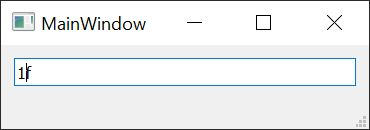
\includegraphics[scale=0.5]{Figures/edit4.jpg}}
  }
  \\
  {}
  &{
  \boxed{
    \textbf{Controller}
  }
  }
  &{}
}
\]
Обратите внимание, что модель в этом случае не просто строка, а строка и позиция курсора.
Потому что окно для редактирования умеет показывать положение курсора для редактирования.
Логически данные (или состояние) хранится только в модели.
View ничего не хранит (логически не хранит, всякое кэширование данных и прочие вспомогательные структуры могут использоваться).
Важно, что только данные из модели являются настоящей правдой.
То есть без модели View не знает что рисовать.
У нее нет дефолтного состояния.
Контроллер -- это просто кусок кода, который принимает команды от пользователя и на основе них вызывает методы у модели.

\paragraph{Виды соединений}

Теперь когда у нас есть три компоненты надо понять как они друг с другом связаны.
Бывают два типа соединения:
\begin{center}
\begin{tabular}{cc}
{
$
\xymatrix{
  {\phantom{\text{Model}}}
  {\save
  [].[dd]*+[F--]\frm{}
  \restore
  } 
  &{\text{View1}}\\
  {\text{Model}}\ar@{-->}[ru]\ar@{-->}[r]\ar@{-->}[rd]&{\text{View2}}\\
  {}&{\text{View3}}\\
}
$
}
&
{
$
\xymatrix{
  {\text{Controller1}}\ar@{->>}[rd]&  {\phantom{\text{Model}}}
  {\save
  [].[dd]*+[F--]\frm{}
  \restore
  }
  \\
  {\text{Controller2}}\ar@{->>}[r]&{\text{Model}}\\
  {\text{Controller3}}\ar@{->>}[ru]&{}\\
}
$
}\vspace{0.5cm}\\
{
$
\xymatrix{
  {\text{Observable}}\ar@{-->}[r]&{\text{Observer}}
}
$
}
&
{
$
\xymatrix{
  {\text{Controller}}\ar@{->>}[r]&{\text{Model}}
}
$
}
\end{tabular}
\end{center}
Соединение представленное слева -- это push уведомления, которые представляют из себя Observalbe/Observer соединения, которое обсуждалось в разделе~\ref{section::Observer}.
Его главная особенность в том, что у нас один источник данных и много слушателей для этих данных.
Соединение справа -- это соединение Host/Handle, которое обсуждалось в разделе~\ref{section::TrackingPtr}.
Его основная особенность, что наоборот может быть много контроллеров на одну модель.

\subsubsection{Модель для MVC}

\paragraph{Обычная модель}

Обычно принято рисовать такую общую картинку для описания того, как соединяются компоненты между собой.
\[
\xymatrix{
  {\phantom{\text{Model}}}
  {\save
  [].[dd]*+[F--]\frm{}
  \restore
  }  
  &{\text{View}}\ar@{-->}[dd]\\
  {\text{Model}}\ar@{-->}[ru]&{}\\
  {}&{\text{Controller}}\ar@{->>}[lu]\\
}
\]
Пунктиром тут обозначены границы ядра программы.
Эта часть вообще не зависит ни от каких графических библиотек.
Эта часть даже не знает, что она является частью интерактивного приложения.
\begin{itemize}
\item
Модель внутри ядра -- основной источник данных.
Как только View присоединилась к Model, то Model тут же отправляет ей свое текущее состояние и View тут же его отрисовывает таким, какое оно есть.
Если у модели что-то поменялось, то она тут же оповещает свою View (или несколько View), чтобы та отобразила ее в текущем состоянии.
К одной модели может быть подсоединено много разных View.
Вы можете пытаться отображать данные в разных форматах в разных окнах или вообще принципиально разных способом.

\item
Контроллер же наоборот управляет моделью по указателю.
Точнее, чтобы соединение было надежным это надо делать через handle.
В данном случае Model является host.
А внутри контроллера содержится handle для управления моделью.
У одной модели может быть много контроллеров.
Например, один контроллер от клавиатуры, а другой от GUI.
Потому тут не подходит Observable/Observer соединение.

\item
И последняя часть -- соединение между View и Controller.
Обычно представляют, что это тоже push уведомления по типу Observer/Observable.
Почему это так.
Ну потому что если пользователь нажал на кнопку экрана, то это возникло какое-то действие, о котором знает View.
И значит она должна сообщить теперь об этом Controller.
Однако так бывает не всегда.
Бывает что источник сигнала не внутри View.
Например ввод с клавиатуры.
\end{itemize}
Когда вы пишите свое интерактивное приложение, вы вряд ли пишите все GUI и Message Driven System-у с нуля сами, вы скорее всего используете готовые решения.
А тогда есть подозрения, что ни одна из библиотек не поддерживает возможности соединяться по Observable/Observer соединению, в особенности используемому вами в вашем проекте.
Потому полезно эту концептуальную картину немного представить в другом виде.

\paragraph{Другая модель}

Вот еще чуть более реалистичная картинка.
\[
\xymatrix{
  {\phantom{\text{Model}}}
  {\save
  [].[dd]*+[F--]\frm{}
  \restore
  }  
  &{\text{View}}\ar[r]&{\text{GUI}}
  {\save
  [].[dd]*+[F--]\frm{}
  \restore
  }\\
  {\text{Model}}\ar@{-->}[ru]&{}&{\text{Library}}\\
  {}&{\text{Controller}}\ar@{->>}[lu]&{\text{Message System}}\ar@{~>}[l]\\
}
\]
Здесь виды соединений:
\[
\xymatrix@R=5pt@C=15pt{
  {\text{Observable}(1)}\ar@{-->}[r]&{\text{Observer}(n)}&  {\text{View}(1)}\ar@{->}[r]&{\text{GUI}(1)}\\
  {\text{Controller}(n)}\ar@{->>}[r]&{\text{Model}(1)}&  {\text{Message System}(1)}\ar@{~>}[r]&{\text{Controller}(n)}\\
}
\]
Давайте прокомментируем соединения.
\begin{enumerate}
\item Model$\to$View -- как и раньше Observable/Observer соединение для поставления данных из модели во View.
Соединение от одной модели к многим View.

\item Controller$\to$Model -- как и раньше соединение по типу Host/Handle для управления моделью.
Соединение от нескольких контроллеров к одной модели.

\item View$\to$GUI.
Если вы используете готовую GUI библиотеку, то для каждого View объекта вы будете использовать библиотечный код для имплементации GUI.
Обычно для одной View вы создаете один объект, представляющей состояние View (состояние графического изображения для пользователя, но НЕ состояние модели).
Это обычно один в один соединение.

\item Message System$\to$Controller.
В интерактивных приложениях обычно используются Message Driven Systems, которые обсуждались в разделе~\ref{section::MDS}.
Любые действия пользователя тогда перерабатываются в сообщения системы.
А потому контроллер должен прослушивать данные сообщения и после этого совершать нужные действия с моделью.
Тут есть такая тонкость.
Все ли необходимые для совершения действия данные прилетают внутри сообщения.
Бывает так, что не все.
А тогда у контроллера должна быть возможность эти данные получить.
А это значит, что он может хранить какие-то указатели или лучше handle-ы на графические компоненты, где должны быть данные.
\end{enumerate}

\subsubsection{Демонстрация как работает MVC}

Давайте вернемся к первой модели в маленьком масштабе из предыдущего примера.
Напомню, что у нас есть простое окно с полем для ввода и изменения текста.
Предположим, что мы поставили курсор и нажали друг за другом клавиши <<1>>, <<f>> и <<$\leftarrow$>>.
Тогда видимое еоведение будет таким
\[
\xymatrix@R=40pt@C=50pt{
  {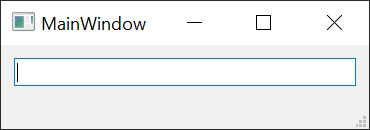
\includegraphics[scale=0.5]{Figures/edit1.jpg}}
  \ar@{|->}[r]^{\boxed{1}}
  &
  {{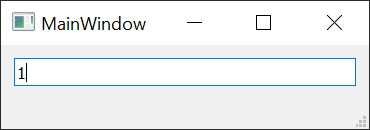
\includegraphics[scale=0.5]{Figures/edit2.jpg}}}
  \ar@{|->}[dl]+(-2,11)|{\boxed{f}}
  \\
  {{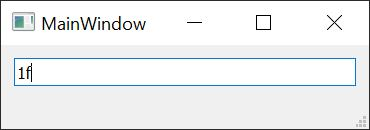
\includegraphics[scale=0.5]{Figures/edit3.jpg}}}
  \ar@{|->}[r]^{\boxed{\leftarrow}}
  &
  {{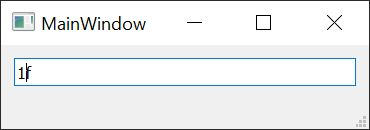
\includegraphics[scale=0.5]{Figures/edit4.jpg}}}
}
\]
Давайте посмотрим, как такая система должна работать по внутренней логике MVC паттерна.
У любой интерактивной программы есть две стадии:
\begin{enumerate}
\item Инициализация всех ресурсов для начала исполнения.

\item Исполнение программы.
\end{enumerate}
Во время первой стадии нам нужно проделать следующее:
\begin{enumerate}
\item Создать Model.

\item Создать View.

\item Создать Controller.

\item Соединить Model$\to$View.

\item Соединить View$\to$Controller.

\item Соединить Controller$\to$Model.
\end{enumerate}
Во время второй стадии собранная система реагирует на сообщения Message Driven System-ы.

Начнем с создания объектов.
В конструкторе нашего приложения мы создаем Model, View и Controller.
Логически будем представлять их так.
\[
\xymatrix{
  {
  \boxed{
  \begin{tabular}{c}
    string:\;""\\
    int:\;0
  \end{tabular}
  }
  }
  %\ar@{-->}[rr]
  &{}&
  {
  \parbox{3cm}{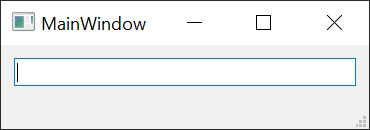
\includegraphics[scale=0.5]{Figures/edit1.jpg}}
  }
  %\ar@{-->}[dl]
  \\
  {}&
  {
  {\boxed{
    \text{Ctrl}
  }}
  }
  %\ar@{->>}[ul]
  &{}
}
\]
Обратите внимание, что сейчас у меня показывается окно с пустым полем для ввода и позицией коретки на нуле.
Однако, это не очень правильное представление.
По хорошему в этом состоянии View просто показывает белое поле без информации.
View лишь знает геометрию поля для ввода, но не его содержание.
И лишь в момент соединения Model и View, данные от модели поступают во View и она их отрисовывает.
\[
\xymatrix{
  {
  \boxed{
  \begin{tabular}{c}
    string:\;""\\
    int:\;0
  \end{tabular}
  }
  }
  \ar@{-->}[rr]^{\text{Оповещение}}
  &{}&
  {
  \parbox{3cm}{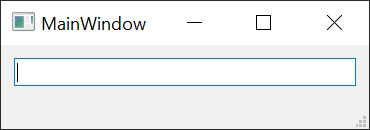
\includegraphics[scale=0.5]{Figures/edit1.jpg}}
  }
  %\ar@{-->}[dl]
  \\
  {}&
  {
  {\boxed{
    \text{Ctrl}
  }}
  }
  %\ar@{->>}[ul]
  &{}
}
\]
Полностью собранная схема будет выглядеть так
\[
\xymatrix{
  {
  \boxed{
  \begin{tabular}{c}
    string:\;""\\
    int:\;0
  \end{tabular}
  }
  }
  \ar@{-->}[rr]
  &{}&
  {
  \parbox{3cm}{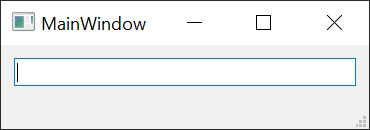
\includegraphics[scale=0.5]{Figures/edit1.jpg}}
  }
  \ar@{-->}[dl]
  \\
  {}&
  {
  \boxed{
    \text{Ctrl}
  }
  }
  \ar@{->>}[ul]
  &{}
}
\]
На этом закончилась стадия конструирования.
Перейдем к стадии обработки сообщений.
На этой стадии мы считаем, что пользователь последовательно выполнил следующие команды
\begin{enumerate}
\item Нажата клавиша <<1>>.

\item Нажата клавиша <<f>>.

\item Нажата клавиша <<$\leftarrow$>> (стрелка влево).
\end{enumerate}
Ниже показана поэтапная схема, отражающая, что происходит в MVC контуре.
Красным обозначается текущая в данный момент операция.
\begin{center}
\newcounter{listitem}
\newcommand{\listitem}{\par\addtocounter{listitem}{1}\noindent\textbf{\arabic{listitem})}\; }
\begin{longtable}{ll}
{
\listitem
\begin{minipage}[\baselineskip]{8cm}
\[
\xymatrix{
  {
  \boxed{
  \begin{tabular}{c}
    string:\;``''\\
    int:\;0
  \end{tabular}
  }
  }
  \ar@{-->}[rr]
  &{}
  &{
  \parbox{3cm}{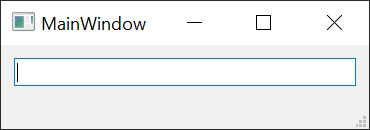
\includegraphics[scale=0.45]{Figures/edit1.jpg}}
  }
  \ar@{-->}@[red][dl]|-{\boxed{1}}
  \\
  {}
  &{
  \boxed{
    \text{Ctrl}
  }
  }
  \ar@{->>}[ul]
  &{}
}
\]
\end{minipage}
}&{
\listitem
\begin{minipage}[\baselineskip]{8cm}
\[
\xymatrix{
  {
  \boxed{
  \begin{tabular}{c}
    string:\;``''\\
    int:\;0
  \end{tabular}
  }
  }
  \ar@{-->}[rr]
  &{}
  &{
  \parbox{3cm}{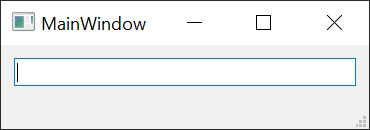
\includegraphics[scale=0.45]{Figures/edit1.jpg}}
  }
  \ar@{-->}[dl]
  \\
  {}
  &{
  \boxed{
    \text{Ctrl}
  }
  }
  \ar@{->>}@[red][ul]
  &{}
}
\]
\end{minipage}
}\\\hline
{
\listitem
\begin{minipage}[\baselineskip]{8cm}
\[
\xymatrix{
  {
  \boxed{
  \begin{tabular}{c}
    string:\;\color{red}{``1''}\\
    int:\;\color{red}{1}
  \end{tabular}
  }
  }
  \ar@{-->}[rr]
  &{}
  &{
  \parbox{3cm}{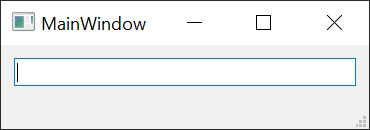
\includegraphics[scale=0.45]{Figures/edit1.jpg}}
  }
  \ar@{-->}[dl]
  \\
  {}
  &{
  \boxed{
    \text{Ctrl}
  }
  }
  \ar@{->>}[ul]
  &{}
}
\]
\end{minipage}
}&{
\listitem
\begin{minipage}[\baselineskip]{8cm}
\[
\xymatrix{
  {
  \boxed{
  \begin{tabular}{c}
    string:\;``1''\\
    int:\;1
  \end{tabular}
  }
  }
  \ar@{-->}@[red][rr]
  &{}
  &{
  \parbox{3cm}{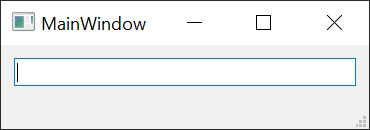
\includegraphics[scale=0.45]{Figures/edit1.jpg}}
  }
  \ar@{-->}[dl]
  \\
  {}
  &{
  \boxed{
    \text{Ctrl}
  }
  }
  \ar@{->>}[ul]
  &{}
}
\]
\end{minipage}
}\\\hline
{
\listitem
\begin{minipage}[\baselineskip]{8cm}
\[
\xymatrix{
  {
  \boxed{
  \begin{tabular}{c}
    string:\;``1''\\
    int:\;1
  \end{tabular}
  }
  }
  \ar@{-->}[rr]
  &{}
  &{
  \parbox{3cm}{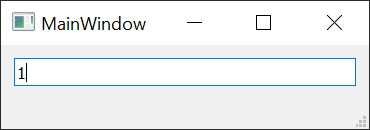
\includegraphics[scale=0.45]{Figures/edit2.jpg}}
  }
  \ar@{-->}[dl]
  \\
  {}
  &{
  \boxed{
    \text{Ctrl}
  }
  }
  \ar@{->>}[ul]
  &{}
}
\]
\end{minipage}
}&{
\listitem
\begin{minipage}[\baselineskip]{8cm}
\[
\xymatrix{
  {
  \boxed{
  \begin{tabular}{c}
    string:\;``1''\\
    int:\;1
  \end{tabular}
  }
  }
  \ar@{-->}[rr]
  &{}
  &{
  \parbox{3cm}{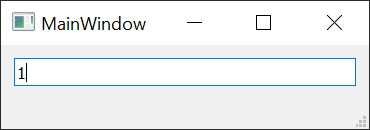
\includegraphics[scale=0.45]{Figures/edit2.jpg}}
  }
  \ar@{-->}@[red][dl]|-{\boxed{f}}
  \\
  {}
  &{
  \boxed{
    \text{Ctrl}
  }
  }
  \ar@{->>}[ul]
  &{}
}
\]
\end{minipage}
}\\\hline
{
\listitem
\begin{minipage}[\baselineskip]{8cm}
\[
\xymatrix{
  {
  \boxed{
  \begin{tabular}{c}
    string:\;``1''\\
    int:\;1
  \end{tabular}
  }
  }
  \ar@{-->}[rr]
  &{}
  &{
  \parbox{3cm}{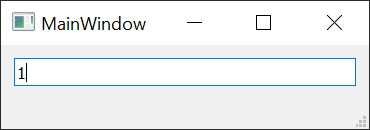
\includegraphics[scale=0.45]{Figures/edit2.jpg}}
  }
  \ar@{-->}[dl]
  \\
  {}
  &{
  \boxed{
    \text{Ctrl}
  }
  }
  \ar@{->>}@[red][ul]
  &{}
}
\]
\end{minipage}
}&{
\listitem
\begin{minipage}[\baselineskip]{8cm}
\[
\xymatrix{
  {
  \boxed{
  \begin{tabular}{c}
    string:\;\color{red}{``1f''}\\
    int:\;\color{red}{2}
  \end{tabular}
  }
  }
  \ar@{-->}[rr]
  &{}
  &{
  \parbox{3cm}{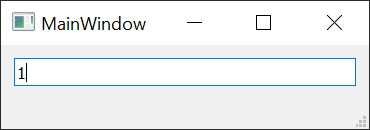
\includegraphics[scale=0.45]{Figures/edit2.jpg}}
  }
  \ar@{-->}[dl]
  \\
  {}
  &{
  \boxed{
    \text{Ctrl}
  }
  }
  \ar@{->>}[ul]
  &{}
}
\]
\end{minipage}
}\\\hline
{
\listitem
\begin{minipage}[\baselineskip]{8cm}
\[
\xymatrix{
  {
  \boxed{
  \begin{tabular}{c}
    string:\;``1f''\\
    int:\;2
  \end{tabular}
  }
  }
  \ar@{-->}@[red][rr]
  &{}
  &{
  \parbox{3cm}{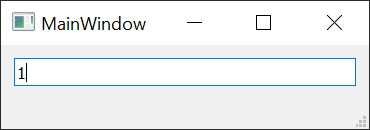
\includegraphics[scale=0.45]{Figures/edit2.jpg}}
  }
  \ar@{-->}[dl]
  \\
  {}
  &{
  \boxed{
    \text{Ctrl}
  }
  }
  \ar@{->>}[ul]
  &{}
}
\]
\end{minipage}
}&{
\listitem
\begin{minipage}[\baselineskip]{8cm}
\[
\xymatrix{
  {
  \boxed{
  \begin{tabular}{c}
    string:\;``1f''\\
    int:\;2
  \end{tabular}
  }
  }
  \ar@{-->}[rr]
  &{}
  &{
  \parbox{3cm}{\includegraphics[scale=0.45]{Figures/edit3.jpg}}
  }
  \ar@{-->}[dl]
  \\
  {}
  &{
  \boxed{
    \text{Ctrl}
  }
  }
  \ar@{->>}[ul]
  &{}
}
\]
\end{minipage}
}\\\hline
{
\listitem
\begin{minipage}[\baselineskip]{8cm}
\[
\xymatrix{
  {
  \boxed{
  \begin{tabular}{c}
    string:\;``1f''\\
    int:\;2
  \end{tabular}
  }
  }
  \ar@{-->}[rr]
  &{}
  &{
  \parbox{3cm}{\includegraphics[scale=0.45]{Figures/edit3.jpg}}
  }
  \ar@{-->}@[red][dl]|-{\boxed{\leftarrow}}
  \\
  {}
  &{
  \boxed{
    \text{Ctrl}
  }
  }
  \ar@{->>}[ul]
  &{}
}
\]
\end{minipage}
}&{
\listitem
\begin{minipage}[\baselineskip]{8cm}
\[
\xymatrix{
  {
  \boxed{
  \begin{tabular}{c}
    string:\;``1f''\\
    int:\;2
  \end{tabular}
  }
  }
  \ar@{-->}[rr]
  &{}
  &{
  \parbox{3cm}{\includegraphics[scale=0.45]{Figures/edit3.jpg}}
  }
  \ar@{-->}[dl]
  \\
  {}
  &{
  \boxed{
    \text{Ctrl}
  }
  }
  \ar@{->>}@[red][ul]
  &{}
}
\]
\end{minipage}
}\\\hline
{
\listitem
\begin{minipage}[\baselineskip]{8cm}
\[
\xymatrix{
  {
  \boxed{
  \begin{tabular}{c}
    string:\;``1f''\\
    int:\;\color{red}{1}
  \end{tabular}
  }
  }
  \ar@{-->}[rr]
  &{}
  &{
  \parbox{3cm}{\includegraphics[scale=0.45]{Figures/edit3.jpg}}
  }
  \ar@{-->}[dl]
  \\
  {}
  &{
  \boxed{
    \text{Ctrl}
  }
  }
  \ar@{->>}[ul]
  &{}
}
\]
\end{minipage}
}&{
\listitem
\begin{minipage}[\baselineskip]{8cm}
\[
\xymatrix{
  {
  \boxed{
  \begin{tabular}{c}
    string:\;``1f''\\
    int:\;1
  \end{tabular}
  }
  }
  \ar@{-->}@[red][rr]
  &{}
  &{
  \parbox{3cm}{\includegraphics[scale=0.45]{Figures/edit3.jpg}}
  }
  \ar@{-->}[dl]
  \\
  {}
  &{
  \boxed{
    \text{Ctrl}
  }
  }
  \ar@{->>}[ul]
  &{}
}
\]
\end{minipage}
}\\\hline
{
\listitem
\begin{minipage}[\baselineskip]{8cm}
\[
\xymatrix{
  {
  \boxed{
  \begin{tabular}{c}
    string:\;``1f''\\
    int:\;1
  \end{tabular}
  }
  }
  \ar@{-->}[rr]
  &{}
  &{
  \parbox{3cm}{\includegraphics[scale=0.45]{Figures/edit4.jpg}}
  }
  \ar@{-->}[dl]
  \\
  {}
  &{
  \boxed{
    \text{Ctrl}
  }
  }
  \ar@{->>}[ul]
  &{}
}
\]
\end{minipage}
}&{
}\\
\end{longtable}
\end{center}
Давайте прокомментируем как это работает.
\begin{enumerate}
\item После нажатия на клавишу <<1>> оповещается соответствующий графический компонент, в нашем случае это поле для ввода текста.
В этот момент поле ввода для текста НЕ меняется, потому что у него нет внутреннего состояния, оно всегда отражает состояние модели.
Вместо этого этот компонент посылает сообщение контроллеру, что нажата клавиша <<1>>.

\item На этом этапе контроллер видит, что клавиша <<1>> дает символ ``1'', который надо поместить в строку внутри модели и сдвинуть коретку на $1$ вперед.

\item На этом слайде красным помечено изменение состояния модели.

\item Как только модель изменила свое состояние, она оповещает всех, кто на нее подписан, чтобы они пришли с ней в одно состояние.
В частности оповещается поле для ввода текста о новом состоянии модели.

\item И вот на этом шаге поле для ввода текста получив новое состояние модели отражает его в виде строки <<1>> и положения картки после цифры $1$.

\item После нажатия на клавишу <<f>>, оповещается графически элемент -- поле для ввода текста.
После чего это поле посылает сигнал контроллеру.

\item Контроллер видит, что эта клавиша дает символ.
И зовет метод модели, который добавляет этот символ в месте расположения каретки.

\item Здесь красным обозначено новое состояние модели.
Теперь хранится строка <<1f>> и новое положение каретки $2$.

\item Теперь модель оповещает текстовое поле о своем новом состоянии.

\item Текстовое поле отражает новое состояние модели.
То есть оно отображает строку <<1f>> и новое положение коретки в конце строки.

\item Теперь после нажатия пользователем клавишы <<$\leftarrow$>> -- стрелка влево, оповещается соответствующий графический компонент -- поле ввода для текста.
Этот компонент посылает сигнал контроллеру.

\item Контроллер видит, что это клавиша отвечает за навигацию по тексту и вызывает у модели метод сдвига коретки влево.

\item Новое положение коретки в модели отмечено красным.
Строка не меняется.

\item Теперь модель оповещает всех о своем новом состоянии.

\item И наконец-то текстовое поле отображает текущую строку <<1f>> и положение коретки между этих двух символов.
\end{enumerate}
Этот пример хорошо показывает общую логику работы MVC.
Все данные хранятся в модели, она единственный источник информации.
View всегда отражает только то, что ей прилетело от модели и логически не имеет своего состояния.
Контроллер же управляет моделью напрямую.

\paragraph{Замечание про Controller}

В такой схеме может показаться странным, что нам нужно использовать View и Controller как две разные сущности.
Потому что все равно все данные из View идут в Controller и потом по этим данным дергается модель.
Причина почему выделяется контроллер -- мы не хотим, чтобы в GUI коде была бизнес логика управления моделью.
Мы не хотим, чтобы GUI зависело от ядра.
Мы хотим, чтобы GUI зависило от данных, которые прилетают из ядра по Observer паттерну, но мы не хотим чтобы были какие-либо другие зависимости.
Чтобы отрезать GUI код от ядра и вводится контроллер.
В этом случае View лишь зависит от двух типов данных: получаемые от модели и отсылаемые контроллеру.
View не принимает никаких решений, не умеет управлять моделью, не содержит никакой логики.
Вся логика управления уходит в Controller.

\subsubsection{MVC и реальность}

Если вы работаете с готовыми графическими библиотеками, то к сожалению или к счастью, они не предоставляют stateless (без состояния) графических компонент (или не всегда их предоставляют).
А потому любой графический компонент или widget в реальной библиотеки сам из себя представляет уже готовый MVC контур запеченый в один объект.
И если вы пытаетесь использовать этот widget как View, у вас получится какая-то такая картинка:
\[
\xymatrix{
  {}&{}&{}&{\text{\textbf{Widget}}}&{}\\
  {}&{}&{\text{M}}\ar@{-->}[rr]
  {\save
  [].[rrd]*+[F-]\frm{}
  \restore
  }
  &{}&{\text{V}}\ar@{-->}[dl]\\
  {\text{Model}}\ar@{-->}@(u,l)[urr]&{}&{}\ar@{-->}@(d,r)[dl]&{\text{C}}\ar@{->>}[ul]&{}\\
  {}&{\text{Ctrl}}\ar@{->>}@(l,d)[ul]&{}&{}&{}\\
}
\]
В бокс справа на картинке объединены внутренности Widget.
При использовании View, которая имеет состояние, вы по сути имеете две модели, которые вам придется согласовывать.
А согласование двух моделей при двустороннем общении -- это всегда огромная проблема.
У вас возникают следующие проблемы
\begin{enumerate}
\item Двойное обновление модели.

\item Гашение обратной связи.
\end{enumerate}
Давайте промоделируем одно оповещение контроллера в схеме представленной выше.
Предположим на пользователь совершил какое-то действие, которое заставило View внутри Widget-а оповестить контроллер внутри Widget-а.
\begin{center}
\setcounter{listitem}{0}
\newcommand{\listitem}{\par\addtocounter{listitem}{1}\noindent\textbf{\arabic{listitem})}\; }
\begin{longtable}{ll}
{
\listitem
\begin{minipage}[\baselineskip]{8cm}
\[
\xymatrix@R=15pt@C=15pt{
  {}&{}&{}&{\textbf{Qt Widget}}&{}\\
  {}&{}&{\text{M}}\ar@{-->}[rr]
  {\save
  [].[rrd]*+[F-]\frm{}
  \restore
  }
  &{}&{\text{V}}\ar@{-->}@[red][dl]\\
  {\text{Model}}\ar@{-->}@(u,l)[urr]&{}&{}\ar@{-->}@(d,r)[dl]&{\text{C}}\ar@{->>}[ul]&{}\\
  {}&{\text{Ctrl}}\ar@{->>}@(l,d)[ul]&{}&{}&{}\\
}
\]
\end{minipage}
}&{
\listitem
\begin{minipage}[\baselineskip]{8cm}
\[
\xymatrix@R=15pt@C=15pt{
  {}&{}&{}&{\textbf{Qt Widget}}&{}\\
  {}&{}&{\text{M}}\ar@{-->}[rr]
  {\save
  [].[rrd]*+[F-]\frm{}
  \restore
  }
  &{}&{\text{V}}\ar@{-->}[dl]\\
  {\text{Model}}\ar@{-->}@(u,l)[urr]&{}&{}\ar@{-->}@(d,r)[dl]&{\text{C}}\ar@{->>}@[red][ul]&{}\\
  {}&{\text{Ctrl}}\ar@{->>}@(l,d)[ul]&{}&{}&{}\\
}
\]
\end{minipage}
}\\\hline
{
\listitem
\begin{minipage}[\baselineskip]{8cm}
\[
\xymatrix@R=15pt@C=15pt{
  {}&{}&{}&{\textbf{Qt Widget}}&{}\\
  {}&{}&{\text{M}}\ar@{-->}@[red][rr]
  {\save
  [].[rrd]*+[F-]\frm{}
  \restore
  }
  &{}&{\text{V}}\ar@{-->}[dl]\\
  {\text{Model}}\ar@{-->}@(u,l)[urr]&{}&{}\ar@{-->}@(d,r)[dl]&{\text{C}}\ar@{->>}[ul]&{}\\
  {}&{\text{Ctrl}}\ar@{->>}@(l,d)[ul]&{}&{}&{}\\
}
\]
\end{minipage}
}&{
\listitem
\begin{minipage}[\baselineskip]{8cm}
\[
\xymatrix@R=15pt@C=15pt{
  {}&{}&{}&{\textbf{Qt Widget}}&{}\\
  {}&{}&{\text{M}}\ar@{-->}[rr]
  {\save
  [].[rrd]*+[F-]\frm{}
  \restore
  }
  &{}&{\text{V}}\ar@{-->}[dl]\\
  {\text{Model}}\ar@{-->}@(u,l)[urr]&{}&{}\ar@{-->}@(d,r)@[red][dl]&{\text{C}}\ar@{->>}[ul]&{}\\
  {}&{\text{Ctrl}}\ar@{->>}@(l,d)[ul]&{}&{}&{}\\
}
\]
\end{minipage}
}\\\hline
{
\listitem
\begin{minipage}[\baselineskip]{8cm}
\[
\xymatrix@R=15pt@C=15pt{
  {}&{}&{}&{\textbf{Qt Widget}}&{}\\
  {}&{}&{\text{M}}\ar@{-->}[rr]
  {\save
  [].[rrd]*+[F-]\frm{}
  \restore
  }
  &{}&{\text{V}}\ar@{-->}[dl]\\
  {\text{Model}}\ar@{-->}@(u,l)[urr]&{}&{}\ar@{-->}@(d,r)[dl]&{\text{C}}\ar@{->>}[ul]&{}\\
  {}&{\text{Ctrl}}\ar@{->>}@(l,d)@[red][ul]&{}&{}&{}\\
}
\]
\end{minipage}
}&{
\listitem
\begin{minipage}[\baselineskip]{8cm}
\[
\xymatrix@R=15pt@C=15pt{
  {}&{}&{}&{\textbf{Qt Widget}}&{}\\
  {}&{}&{\text{M}}\ar@{-->}[rr]
  {\save
  [].[rrd]*+[F-]\frm{}
  \restore
  }
  &{}&{\text{V}}\ar@{-->}[dl]\\
  {\text{Model}}\ar@{-->}@(u,l)@[red][urr]&{}&{}\ar@{-->}@(d,r)[dl]&{\text{C}}\ar@{->>}[ul]&{}\\
  {}&{\text{Ctrl}}\ar@{->>}@(l,d)[ul]&{}&{}&{}\\
}
\]
\end{minipage}
}\\\hline
{
\listitem
\begin{minipage}[\baselineskip]{8cm}
\[
\xymatrix@R=15pt@C=15pt{
  {}&{}&{}&{\textbf{Qt Widget}}&{}\\
  {}&{}&{\text{M}}\ar@{-->}@[red][rr]
  {\save
  [].[rrd]*+[F-]\frm{}
  \restore
  }
  &{}&{\text{V}}\ar@{-->}[dl]\\
  {\text{Model}}\ar@{-->}@(u,l)[urr]&{}&{}\ar@{-->}@(d,r)[dl]&{\text{C}}\ar@{->>}[ul]&{}\\
  {}&{\text{Ctrl}}\ar@{->>}@(l,d)[ul]&{}&{}&{}\\
}
\]
\end{minipage}
}&{
\listitem
\begin{minipage}[\baselineskip]{8cm}
\[
\xymatrix@R=15pt@C=15pt{
  {}&{}&{}&{\textbf{Qt Widget}}&{}\\
  {}&{}&{\color{red}{\text{M}}}\ar@{-->}[rr]
  {\save
  [].[rrd]*+[F-]\frm{}
  \restore
  }
  &{}&{\text{V}}\ar@{-->}[dl]\\
  {\color{red}{\text{Model}}}\ar@{-->}@(u,l)@[red][urr]&{}&{}\ar@{-->}@(d,r)[dl]&{\text{C}}\ar@{->>}[ul]&{}\\
  {}&{\text{Ctrl}}\ar@{->>}@(l,d)[ul]&{}&{}&{}\\
}
\]
\end{minipage}
}\\
\end{longtable}
\end{center}
Давайте прокомментируем, что тут происходит.
Если мы верим, что Widget функционирует как MVC контур (раз он содержит состояние), то мы ожидаем следующее поведение.
\begin{enumerate}
\item В начале Widget получает от экосистемы сообщение о действиях пользователя.
А именно View объект внутри Widget-а оповещается об этом событии.
После чего View объект должен оповестить внутренний контроллер, чтобы обновить свое состояние.

\item Когда внутренний контроллер получает оповещение, он дергает внутреннюю модель, чтобы она обновилась.

\item Когда модель обновилась она совершает два действия.
Первое -- оно оповещает внутренний View объект, чтобы отразить свое новое состояние.

\item Второе действие -- послать сигнал наружним объектам.
В данном случае внешнему контроллеру Ctrl.

\item Теперь контроллер оповещает нашу модель Model.

\item Модель меняет свое состояние и оповещает Widget.

\item Widget меняет состояние внутренней модели в соответствии с состоянием, которое пришло от Model.
А раз обновилось внутреннее состояние, то надо опять оповестить внутренюю View.

\item Как мы видим, в ребре между двумя моделями оказалось, двойное обновление внутренней модели одними и теми же данными.
Из-за чего происходит двойное обновление View внутри Widget.
Эта проблема связана с тем, что модель снаружи и внутри Widget общаются в двустороннем порядке.
\end{enumerate}
Поведение описанное выше может быть как желательным, так и не желательным.
Например, если мы использовали statefull Widget мы не хотим двойное обновление View объекта, чтобы экран лишний раз не мерцал.
Ну и в целом это логически плохо.

Какие есть методы решения этой проблемы.
\begin{enumerate}
\item Одно из частных решений -- поставить гаситель обратной связи или Suppressor на стороне M.
Это значит, что когда мы оповещаем всех, мы перестаем слушать входящие сигналы.
К сожалению это работает только для блокирующих вызовов.
Кроме того, может быть опасность пропустить нужный сигнал от модели.

\item Другой подход -- поместить некую логику оповещения на стороне Model.
То есть теперь Model должна знать кого оповещать а кого нет.
Это достаточно сложная задача, потому что контроллеру надо передавать модели данные об отправители и Model теперь должна не просто обновлять свое состояние, но еще и принимать решение кого оповещать.
Это опасно рассинхроном состояний.

\item Можно поместить логику обработки оповещений на стороне внутренней модели M.
То есть внутренняя модель смотри прилетевшие данные и проверяет отличается ли ее состояние от пришедшего.
Это логически самое правильное решение, но тогда нам надо уметь очень быстро считать разницу между состояниями.
Иначе этот подход может оказаться очень дорогим для исполнения.
\end{enumerate}
На удивление все становится сильно проще и удобнее, если мы переходим к неблокирующим соединениям между компонентами.
В данном случае неблокирующий observer паттерн (можно посмотреть раздел~\ref{section::ObserverNonBlocking}).
В этом случае общение компонент можно рассматривать как общение по сети.
И для корректного общения нужен грамотный протокол общения, который решает все проблемы подобного характера.
Никакие кустарные заплатки в виде suppressor-ов в нем не потребуются.

\subsubsection{Пример 1 использования MVC}

Здесь я хочу привести пример программы по анализу качества печати, которую я разрабатывал.
Начну со скриншота, чтобы можно было что-то объяснять.
\begin{center}
\includegraphics[scale=0.355]{Figures/appfull.JPG}
\end{center}
Давайте в общих чертах объясню, что здесь происходит.
Данная программа представляет из себя всего одно окно, которое вы видите на скриншоте выше.
Программа умеет находиться в двух режимах:
\begin{enumerate}
\item Режим перехвата клавиватуры.
В свернутом режиме, программа перехватывает весь ввод пользователя.

\item Режим анализа.
В развернутом режиме, программе не прослушивает клавиатуру, вместо этого она дает возможность посмотреть информацию о уже записанных данных, которые были перехвачены ранее.
\end{enumerate}
При переходе от прослушивающего состояния в состояние анализа все накопленные данные сгружаются в ядро программы.
Вся информация о наборе хранится в виде сессий.
Теперь опишем компоненты графического интерфейса.
\begin{enumerate}
\item
Слева вы видите список сессий, где отражено несколько первых клавиш нажатых в данную сессию, ее длина в количестве нажатых клавиш и какая сессия сейчас активна.
\begin{center}
\includegraphics[scale=0.5]{Figures/SessView.JPG}
\end{center}

\item Над панелью для выбора сессий находится панель выбора режима для отображения перехваченного набора.
\begin{center}
\includegraphics[scale=0.5]{Figures/textmodev.JPG}
\end{center}
Данный режим влияет на отображение сессии в текстовом окне описанном в пункте~\ref{item::TextView}.
Есть три режима
\begin{enumerate}
\item Сырой.
В нем отображаются все клавиши которые были нажаты независимо от того дают они символы или нет.

\item Полный.
В этом режиме отображаются только напечатанные символы включая все удаленные.
Удаленные символы подсвечиваются специальным образом.

\item Напечатанный.
В этом режиме отображается только конечный текст, который был напечатан без учета стертых символов.
\end{enumerate}

\item
\label{item::TextView}
Сверху по центру расположено текстовое окно предоставляющее информацию о перехваченной сессии.
\begin{center}
\includegraphics[scale=0.5]{Figures/TextView.JPG}
\end{center}

\item Ниже идет график плотности скорости.
\begin{center}
\includegraphics[scale=0.5]{Figures/plotView.JPG}
\end{center} 
Программа трактует скорость нажатия клавиши как случайную величину.
В данном окне приведена плотность распределения данной случайной величины.

\item Справа от текстового окна располагается окно статистики.
\begin{center}
\includegraphics[scale=0.5]{Figures/StatView.JPG}
\end{center}
Самый интересный параметр -- предпоследний параметр -- это пик плотности распределения скорости.
Этот параметр хорошо характеризует скорость физических возможностей наборщика.

\item В самом низу находится клавишная схема, на которой отображается каким пальцем какая клавиша и в какой временной промежуток была нажата.
\begin{center}
\includegraphics[scale=0.5]{Figures/DiagView.JPG}
\end{center}
\end{enumerate}
Тут стоит сказать, что от выбора текстового режима зависят: текстовое окно, график плотности и клавишная схема.
Вот пример как будет выглядеть та же самая сессия а напечатанном режиме.
\begin{center}
\includegraphics[scale=0.355]{Figures/appprint.JPG}
\end{center}
И в сыром режиме
\begin{center}
\includegraphics[scale=0.355]{Figures/appraw.JPG}
\end{center}
Видно, что в этом режиме появляются символы пробела, символы для backspace-а, для шифтов и прочие.

Давайте я продемонстрирую как выглядит часть приложения с точки зрения MVC.
\[
\resizebox{12cm}{!}{
\xymatrix@R=10pt{
  {}&{\parbox{1.5cm}{\includegraphics[scale=0.5]{Figures/SessView.JPG}}}\ar@{-->}[dl]&{}&{\parbox{1.5cm}{\includegraphics[scale=0.5]{Figures/textmodev.JPG}}}\ar@{-->}[dl]&{\parbox{3cm}{\includegraphics[scale=0.5]{Figures/TextView2.JPG}}}&{}&{\parbox{2cm}{\includegraphics[scale=0.5]{Figures/StatView.JPG}}}&{}\\
  {\text{Ctrl}}\ar@{->>}[dr]&{}&{\text{Ctrl}}\ar@{->>}[dr]&{}&{}&{}&{}&{}\\
  {}\ar@{-->}[r]&{\text{Selector}}
  {\save
  [].[rrrrd]*+[F--]\frm{}
  \restore
  }
  \ar@{-->}[rr]\ar@{-->}[uu]&{}&{\text{Text}}\ar@{-->}[d]\ar@{-->}[r]\ar@{-->}[uu]\ar@{-->}[uur]
  &{\text{Math}}\ar@{-->}[r]\ar@{-->}[rddd]+(0,9)&{\text{Stat}}\ar@{-->}[uur]&{}&{}\\
  {}&{}&{\text{Layout}}\ar@{-->}[r]&{\text{Scheme}}\ar@{-->}[ddl]+(0,9)&{}&{\phantom{\text{Plot}}}&{}&{}\\
  {}&{}&{}&{}&{}&{}&{}\\
  {\parbox{1cm}{\includegraphics[scale=0.3]{Figures/DiagView.JPG}}}&{}&{}&{}&{\makebox[0.1cm][r]{\parbox{1cm}{\includegraphics[scale=0.35]{Figures/plotView.JPG}}}}&{}&{}&{}\\
}
}
\]
Давайте я прокомментирую диаграмму выше.
\begin{itemize}
\item Часть выделенная пунктиром в центре -- это часть ядра программы.
Эта часть ничего не знает про графические библиотеки и способна работать без GUI.

\item Пунктирная стрелка слева ведет из другой части ядра, которая нам сейчас не очень важна, ибо в той части не используется MVC.

\item Ядро из себя представляет пайплайн, по которому данные проходят слева направо и после этого сообщаются пользователю через GUI.

\item Блок Selector выбирает текущую сессию для анализа.
Можно видеть MVC контур вокруг этого блока.
Selector является моделью в этом контуре.

\item Блок Text -- текстовый модуль.
Его задача хранить текущий режим и текст, который необходимо отобразить в текстовом окне.
Тут видно, что текстовое окно просто получает новые данные и через него нет возможности управления.
А выбор текстового режима -- это еще один MVC контур.

\item Блок Scheme -- модуль, который по распальцовке заданной пользователем и текущему режиму показывает диаграмму распределения нажатий по пальцам во времени.
Сама распальцовка хранится в модуле Layout и задается пользователем заранее.

\item Блок Math вычисляет плотность распределения скорости набора.
Он оповещает View отображающую плотность.

\item И в конце идет блок Stat, который является модулем статистики.
Он получает всю информацию из всех предыдущих модулей, вычисляет некую статистику и отображает ее в окне для статистики.
\end{itemize}
На этой диаграмме не отображены некоторые мелочи, как например выбор способа вычисления плотности распределения или локализация текста в элементах GUI.
Однако, я надеюсь, что эта схема хотя бы в общих чертах дает понять, как можно собирать подобное интерактивное приложение.
Так же отмечу, что все вызовы между компонентами блокирующие.
Это не очень хорошо, но это не сложно исправить имея value semantics для данных пересылаемых в observer паттерне.
Если вам интересна более детальная информация, то можно изучить \href{https://github.com/DimaTrushin/TypingAnalysis}{репозиторий} с проектом.
Там можно найти дизайн документацию с более подробным описанием происходящего.

\subsubsection{Пример 2 использования MVC}

Еще один пример, который я хочу привести -- это простая программа, которая показывает пользователю поле с двумя фишками и эти фишки можно двигать только на соседние клетки по вертикали и горизонтали.
Больше ничего делать нельзя.
Как обычно приведу скриншот в самом начале.
\begin{center}
\includegraphics[scale=0.6]{Figures/Game1.JPG}
\end{center}
Ожидаемое поведение программы такое.
Вы можете подцепить курсором фишку и перемещать ее держа зажатой левую клавишу мыши.
В момент перемещения захваченной фишки проигрывается настраиваемая анимация.
При отпускании фишки программа пытается поставить ее на указанное поле.
Если шаг сделать не возможно, то фишка возвращается в исходное состояние, откуда она была захвачена.

Важно понять, что в данном случае у нас не одна, а две модели.
\begin{enumerate}
\item Первая модель знает размер поля, расположение на нем фишек и правила, по которым фишкам можно ходить.
Эта модель оперирует целыми координатами фишек, обозначающие столбец и строку, где находится фишка.
Она ничего не знает про отображение поля, про фишки, про цвета, анимацию и прочее.
Это как бы <<внутренняя логика игры>>.

\item Вторая модель -- это геометрическая модель.
Дело в том, что в первой модели не достаточно информации для того, чтобы ее отрисовать.
Например не ясно каким цветом и как рисовать поле, какие должны быть размеры клеток, какие размеры, цвет и форма фишек.
Кроме того, при захвате фишки курсором она может находиться в состоянии, не имеющем смысла для модели игры.
Потому для отображения геометрии мы используем вторую модель.
\end{enumerate}
Схематически устройство программы выглядит так.
\[
\xymatrix{
  {\verb"model"}\ar@{-->}[rr]
  	{
	\save
   [].[]*+[F-:<3pt>]\frm{}
   \restore
	}
	{
	\save
   []+(-10,6).[drrrr]*+(3,0)++[F-:<3pt>]\frm{}
   \restore
	}
  &{}&{\verb"gmodel"}\ar@{-->}[rr]\ar@{-->}[dl]
      	{
	\save
   [].[]*+[F-:<3pt>]\frm{}
   \restore
	}
  &{}&{\verb"view"}\ar@{-->}[dl]
      	{
	\save
   [].[]*+[F-:<3pt>]\frm{}
   \restore
	}
  \\
  {}&{\verb"ctrl"}\ar@{->>}[lu]
      	{
	\save
   [].[]*+[F-]\frm{}
   \restore
	}
  &{}&{\verb"gctrl"}\ar@{->>}[lu]
      	{
	\save
   [].[]*+[F-]\frm{}
   \restore
	}
  &{}\\
}
\]
Давайте опишем все ее компоненты.
\begin{itemize}
\item model.
Это первая модель которая отвечает за
\begin{enumerate}
\item состояние поля

\item позиции фишек на поле

\item правила как фишки могут ходить
\end{enumerate}

\item gmodel.
Это вторая геометрическая модель.
Она отвечает за:
\begin{enumerate}
\item Система координат на плоскости.

\item Изображение поля

\item Изображение фишек

\item Анимация фишек при захвате

\item Информация какая фишка сейчас выбрана и является активной
\end{enumerate}

\item view.
Это View компонент.
Он не содержит состояния и лишь отрисовывает текущее состояние gmodel.

\item gctrl.
Контроллер управления геометрической моделью.
Позволяет
\begin{enumerate}
\item Захватить фишку при зажатии левой клавиши мыши.
При этом данная фишка становится активной в геометрической модели.

\item Двигать гоеметрическое представление активной фишки.

\item Отпустить захваченную фишку.
При этом фишка перестает быть активной.
\end{enumerate}

\item ctrl.
Это контроллер, который идет от геометрической модели к обычной модели.
Когда пользователь перетащил изображение фишки куда-то, гометерическая модель должна попросить обычную модель попытаться сделать предлагаемый ход.
И это управление делается через данный контроллер.
\end{itemize}
Давайте скажу пару слов по поводу поведения в такой схеме.
Если пользователь отпускает фишку в геометрической модели, то она оповещает View, чтобы та показала, где фишка остановилась.
Но сразу после этого оповещается контроллер модели, который дергает у модели метод, пытающийся сходить фишкой так, как просит геометрическая модель.
Далее модель либо ходит фишкой как сказано, либо отвергает действие.
Но в любом случае после этого она оповещает всех, кто на нее подписан.
В данном случае она оповещает геометрическую модель.
Которая при получении новых данных начинает отражать состояние модели, где фишка либо перемещена на новое поле, либо вернулась назад.
После чего оповещается View, чтобы отрисовать состояние геометрической модели.
Таким образом мы как бы оповещаем View дважды, но это нас устраивает, потому что одно оповещение -- это точка сброса фишки, а другое оповещение -- это исправленное состояние геометрической модели после попытки сделать ход.

\paragraph{Архитектура приложения}

Визуально архитектуру приложения можно представлять себе так.
\[
\xymatrix@R=15pt{
  {\verb"App"}
    {
	\save
   [].[d]*+[F-:<3pt>]\frm{}
   \restore
	}
  &{}&{}&{}\\
  {\verb"u\_ptr"}\ar[r]+(-13,0)&{}
    {
	\save
   []+(-13,4).[dddddrr]*+(8,0)+[F-:<3pt>]\frm{}
   \restore
	}
  &{\verb"AppImpl"}&{}\\
  {}&{\verb"AppKernel"}
  {
	\save
   [].[ddd]*+[F-:<3pt>]\frm{}
   \restore
	}
  &{}&{\verb"AppGui"}
  {
	\save
   [].[d]*+[F-:<3pt>]\frm{}
   \restore
	}
  \\
  {}&{\verb"model"}\ar@{-->}@<3ex>@/^/[dd]&{}&{\verb"view"}\ar@{-->}@(d,r)[dddl]\\
  {}&{\verb"ctrl"}\ar@{->>}[u]&{}&{}\\
  {}
  &{\verb"gmodel"}\ar@{-->}[u]\ar@{-->}[rruu]&{}&{}\\
  {}&{}&{\verb"gctrl"}\ar@{->>}@(l,d)[lu]
  &{}\\
}
\]
Давайте про комментируем, что тут происходит.
\begin{itemize}
\item Объект \verb"App" -- это главный объект нашего приложения.
Для него используется Pimpl (см. раздел~\ref{section::Pimpl}), чтобы разгрузить стек вызовов.

\item Вся имплементация спрятана внутрь \verb"AppImpl".
При этом для улучшения локальности мы выделяем в имплементации два раздела посвященных ядру и GUI.

\item \verb"AppKernel" -- кусок \verb"AppImpl", в котором находятся компоненты ядра.
Технически это базовый класс \verb"AppImple".
В данном случае наследование используется как композиция.
Тут живут model, gmodel и ctrl.

\item \verb"AppGui" -- кусок \verb"AppImpl", в котором находятся все GUI компоненты.
В данном случае это просто view компонента.

\item Контроллер gctrl должен соединять GUI и ядро.
Потому он располагается в \verb"AppImpl" непосредственно.
\end{itemize}
В коде это выглядит так.
\begin{center}
\begin{tabular}{c}
\begin{tabular}{cc}
{
\begin{minipage}[\baselineskip]{8cm}
\begin{cppcode}[numbers = none]
class AppKernel {
  AppKernel()
   : ctrl_(&model_) {
    model_.subscribe(gmodel.port());
    gmodel_.subscribe(ctrl_.port());
  }
protected:
  Model model_;
  GModel gmodel_;
  Ctrl ctrl_;
};
\end{cppcode}
\end{minipage}
}
&
{
\begin{minipage}[\baselineskip]{8cm}
\begin{cppcode}[numbers = none]
class MainWindow {
public:
  View* view();
private:
  View view_;
};

class AppGui {
protected:
  MainWindow window_;
};
\end{cppcode}
\end{minipage}
}
\end{tabular}
\\
\begin{minipage}[\baselineskip]{8cm}
\begin{cppcode}
class AppImpl : AppKernel, AppGui {
public:
  AppImpl() : gctrl_(&gmodel_) {
    gmodel_.subscribe(view()->port());
    view()->subscribe(gctrl_.port());
  }
protected:
  GCtrl gctrl_;
};
\end{cppcode}
\end{minipage}
\end{tabular}
\end{center}
Структура здесь в точности такая как описано выше.
Надо лишь прокомментировать как работают конструкторы.
\begin{enumerate}
\item \verb"AppKernel" в своем конструкторе соединяет компоненты ядра.
Причем в этом дизайне у меня контроллер приваривается к модели в своем конструкторе.
А observable/observer порты надо соединить в теле конструктора.

\item \verb"AppGui" содержит одну компоненту -- основное окно, в котором располагается \verb"view" объект.
Основное окно собирается из Qt кода.

\item Далее все компоненты соединяются в \verb"AppImpl".
С помощью наследования я включаю ядро и GUI часть в имплементацию.
А потом в конструкторе делаю все оставшиеся соединения.
\end{enumerate}

Код приложения можно найти в \href{https://github.com/DimaTrushin/InteractiveGUI}{репозитории}.

\paragraph{Другая вариация приложения}

У этого приложения можно легко сделать вариацию с любым количеством view и геометрических моделей.
Очень полезно понимать, что будет происходить при разных вариациях их соединения.
Начну как обычно со скриншота.
\begin{center}
\includegraphics[scale=0.4]{Figures/Game2.JPG}
\end{center}
В этом случае поля слева синхронизированы на уровне геометрической модели.
А поле справа имеет свою геометрическую модель.
Нижнее поле без контроллера, через него управлять нельзя.
Если захватить фишку на левом поле и двигать захваченную фишку по полю, то ее движение будет видно только на двух левых полях.
Но если фишку отпустить на клетку допустимого хода, то обновятся все три поля разом.
Аналогично, если мы захватим фишку на правом поле, то ее перемещение будет видно только на нем, но когда мы сделаем ход, то обновятся все три поля.

Вот схема соединения объектов.
\[
\xymatrix@R=15pt{
  {}
     {\save
  []+(-10,5).[ddddddrrrr]*+(4,0)+[F-:<3pt>]\frm{}
  \restore
  }
  &{}&{\verb"AppImpl"}&{}&{}\\
 {}
   {\save
  []+(-8,5).[dddddrr]*+(7,0)+[F-:<3pt>]\frm{}
  \restore
  }
 &{\verb"AppKernel"}&{}&{}&{\verb"AppGui"}
    {\save
  []+(-8,5).[ddddd]*+(1,0)+[F-:<3pt>]\frm{}
  \restore
  }
 \\
  {}
  &{\verb"ctrl1"}\ar@{->>}[ldd]
    {\save
  [].[]*[F-:<3pt>]\frm{}
  \restore
  }
  &{}&{\verb"gctrl1"}\ar@{->>}[ld]
    {\save
  [].[]*[F-:<3pt>]\frm{}
  \restore
  }
  &{\verb"view1"}
  \ar@{-->}@/_/[l]
    {\save
  [].[]*[F-:<3pt>]\frm{}
  \restore
  }
  \\
  {}&{}&{\verb"gmodel1"}
  \ar@{-->}[lu]
  \ar@{-->}@/_/[urr]
  \ar@{-->}@/^/[drr]
    {\save
  [].[]*[F-:<3pt>]\frm{}
  \restore
  }
  &{}&{}\\
  {\verb"model"}
  \ar@{-->}[rru]
  \ar@{-->}[rrd]
  {\save
  [].[]*[F-:<3pt>]\frm{}
  \restore
  }
  &{}&{}&{}
  &{\verb"view2"}
    {\save
  [].[]*[F-:<3pt>]\frm{}
  \restore
  }
  \\
  {}&{}&{\verb"gmodel2"}
    \ar@{-->}[ld]
  \ar@{-->}@/^/[drr]
    {\save
  [].[]*[F-:<3pt>]\frm{}
  \restore
  }
  &{}&{}\\
  {}&{\verb"ctrl2"}\ar@{->>}[luu]
    {\save
  [].[]*[F-:<3pt>]\frm{}
  \restore
  }
  &{}&{\verb"gctrl2"}\ar@{->>}[lu]
    {\save
  [].[]*[F-:<3pt>]\frm{}
  \restore}&{\verb"view3"}
    \ar@{-->}@/^/[l]
  {\save
  [].[]*[F-:<3pt>]\frm{}
  \restore
  }
  \\
}
\]
Эта диаграмма напрямую транслируется в код, потому я не буду его тут приводить.

\paragraph{Точка входа в программу}

Данное приложение собиралось в экосистеме Qt с использованием не блокирующего Observer Pattern.
Вот как выглядит функция \verb"main"
\begin{cppcode}
#include "Application.h"
#include "Except.h"
#include "QRunTime.h"

int main(int argc, char* argv[]) {
  QApp::QRunTime runtime(argc, argv);
  try {
    QApp::Application app;
    runtime.exec();
  } catch (...) {
    QApp::Except::react();
  }
  return 0;
}
\end{cppcode}
Сделаем несколько замечаний:
\begin{enumerate}
\item \verb"QRunTime" -- это наша надстройка над Qt runtime-ом, которая позволяет общению неблокирующего observer-а.
Этот объект в начале функции \verb"main" инициализирует всю экосистему и запускает event loop вызовом функции \verb"exec".

\item \verb"Application" -- это класс нашего приложения.
Он является пассивным объектом в Qt экосистеме.
Он ничего не выполняет сам, он и его компоненты лишь реагируют на Qt сообщения и посылают свои.

\item Обратите внимание, что функция \verb"main" ничего не делает сама.
Она всю работу делегирует другим объектам.
Даже обработку исключений.

\item Одна из задач функции \verb"main" -- не допустить утекания исключений в OS.
Это нужно для того, чтобы отличить ошибки которые возникли в программе из-за самой программы от ошибок, которые возникли в программе из-за операционной системы.
\end{enumerate}
При этом обработка исключений выглядит так
\begin{cppcode}
#include "Except.h"
#include <QDebug>
#include <exception>

namespace QApp {
namespace Except {
void react() noexcept {
  try {
    throw;
  } catch (std::exception& e) {
    qDebug() << "Exception: " << e.what();
  } catch (...) {
    qDebug() << "Enknown Exception!";
  }
}
} // namespace Except
} // namespace QApp
\end{cppcode}
Функция react будет вызвана внутри блока \verb"catch", а значит в этот момент есть активное исключение.
Чтобы его еще раз поймать, мы просто внутри \verb"try" блока делаем \verb"throw" без аргументов.
И уже после в разных видах \verb"catch" ловим исключения и реагируем на них.
Все это замечательно за одним большим исключением: Qt не разрешает бросать исключения в event loop.
Это связано с тем, что Qt изначально не планировал поддерживать исключения.
Как мы понимаем сейчас это большая ошибка.
Все новые компоненты Qt пишутся в парадигме exception safe.
Однако, все ключевые компоненты ядра все еще не поддерживают бросание исключений и это большой геморрой.

\subsubsection{MVVM}

Теперь я хочу поговорить о паттерне Model/View/View-Model.
Прежде чем к нему переходить, давайте вспомним наш пример с Widget-ом, который имел внутреннее состояние.
\[
\xymatrix{
  {}&{}&{}&{
  \textbf{Widget}
  }&{}\\
  {}&{}&{
  \phantom{\text{V}}\text{M}
  }
  \ar@{-->}@<0.6ex>[rr]
  {\save
  [].[rrd]*++[F-]\frm{}
  \restore
  }
  &{}&{
  V
  }
  {\save
  [].[d]*++\frm{}
  \restore
  }
  \ar@{-->}[dl]
  \\
  {
  \text{Model}
  }
  \ar@{-->}@(u,l)[urr]
  &{}&{\phantom{\text{Model}}}
  \ar@{-->}@(d,r)[dl]
  &{
  \text{C}
  }
  \ar@{->>}[ul]
  &{\phantom{\text{C}}}
  \\
  {}&{
 \text{Ctrl}
  }
  \ar@{->>}@(l,d)[ul]
  &{}&{}&{}\\
}
\]
Теперь я хочу помодифицировать чуть-чуть эту конструкцию.
Так как внутри Widget-а у нас view оповещает только один контроллер, то в самом начале их можно слить в одну сущность.
\[
\xymatrix{
  {}&{}&{}&{\textbf{Widget}}&{}\\
  {}&{}&{\phantom{\text{V}}\text{M}}\ar@{-->}@(d,r)[ddl]\ar@{-->}@<0.6ex>[rr]
  {\save
  [].[rr]*++[F-]\frm{}
  \restore
  }
  &{}&{\text{V}}\ar@{->>}@<0.6ex>[ll]\\
  {\text{Model}}\ar@{-->}@(u,l)[urr]&{}&{\phantom{\text{Model}}}&{}&{\phantom{\text{C}}}\\
  {}&{\text{Ctrl}}\ar@{->>}@(l,d)[ul]&{}&{}&{}\\
}
\]
Теперь можно вынуть внутреннюю модель наружу, оставив общение с внутренностями Widget-а через фиксированный интерфейс.
\[
\xymatrix{
  {}&{}&{}&{\textbf{Widget}}&{}\\
  {}&{}&{\text{VM}}\ar@{-->}@<0.6ex>[rr]
  {\save
  [].[rr]*++[F-]\frm{}
  \restore
  }
  &{}&{\text{V}}\ar@{->>}@<0.6ex>[ll]\\
  {\text{Model}}\ar@{-->}[rr]+(-2,0)&{}&{\phantom{\text{od}}\text{M}\phantom{\text{el}}}\ar@{->}[u]\ar@{-->}@(d,r)[dl]&{}&{}\\
  {}&{\text{Ctrl}}\ar@{->>}@(l,d)[ul]&{}&{}&{}\\
}
\]
Ну а теперь просто нет необходимости во второй модели.
И мы получаем.
\[
\xymatrix{
  {}&{}&{}&{\textbf{Widget}}&{}\\
  {}&{}&{\text{VM}}\ar@{-->}@<0.6ex>[rr]
  {\save
  [].[rr]*++[F-]\frm{}
  \restore
  }
  &{}&{\text{V}}\ar@{->>}@<0.6ex>[ll]\\
  {\phantom{\text{Model}}}&{}&{\text{Model}}\ar@{->}[u]&{}&{}\\
  {}&{\phantom{\text{Ctrl}}}&{}&{}&{}\\
}
\]
Давайте я прокомментирую, что тут произошло.
Для того, чтобы сделать view stateless нам нужно как-то внутри view получать данные из модели.
Понятно, что их можно получать по observer паттерну, но проблема в том, в каком формате они должны быть.
Так вот формат данных для view -- это первое что надо фиксировать.
Кроме того, если мы хотим управлять произвольной моделью не зная, как она устроена, то нам нужна вспомогательная прослойка, которая на картинке изображена как VM.
Это по сути интерфейс для общения с моделью.
Это не обязательно интерфейс в смысле наследования с виртуальными функциями.
Это может быть стирающий указатель (см. раздел~\ref{section::RefErasure}).
В такой модели интерфейс View Model соединяется напрямую с View, потому что ей больше не с кем соединяться.
А Model подключается к View Model уже внешне.
Такой подход называется Model/View/View-Model.
Важно понимать, что он ни в коем случае не отменяет MVC.
